\documentclass[twoside]{book}

% Packages required by doxygen
\usepackage{fixltx2e}
\usepackage{calc}
\usepackage{doxygen}
\usepackage[export]{adjustbox} % also loads graphicx
\usepackage{graphicx}
\usepackage[utf8]{inputenc}
\usepackage{makeidx}
\usepackage{multicol}
\usepackage{multirow}
\PassOptionsToPackage{warn}{textcomp}
\usepackage{textcomp}
\usepackage[nointegrals]{wasysym}
\usepackage[table]{xcolor}

% NLS support packages
\usepackage[ngerman]{babel}

% Font selection
\usepackage[T1]{fontenc}
\usepackage[scaled=.90]{helvet}
\usepackage{courier}
\usepackage{amssymb}
\usepackage{sectsty}
\renewcommand{\familydefault}{\sfdefault}
\allsectionsfont{%
  \fontseries{bc}\selectfont%
  \color{darkgray}%
}
\renewcommand{\DoxyLabelFont}{%
  \fontseries{bc}\selectfont%
  \color{darkgray}%
}
\newcommand{\+}{\discretionary{\mbox{\scriptsize$\hookleftarrow$}}{}{}}

% Page & text layout
\usepackage{geometry}
\geometry{%
  a4paper,%
  top=2.5cm,%
  bottom=2.5cm,%
  left=2.5cm,%
  right=2.5cm%
}
\tolerance=750
\hfuzz=15pt
\hbadness=750
\setlength{\emergencystretch}{15pt}
\setlength{\parindent}{0cm}
\setlength{\parskip}{3ex plus 2ex minus 2ex}
\makeatletter
\renewcommand{\paragraph}{%
  \@startsection{paragraph}{4}{0ex}{-1.0ex}{1.0ex}{%
    \normalfont\normalsize\bfseries\SS@parafont%
  }%
}
\renewcommand{\subparagraph}{%
  \@startsection{subparagraph}{5}{0ex}{-1.0ex}{1.0ex}{%
    \normalfont\normalsize\bfseries\SS@subparafont%
  }%
}
\makeatother

% Headers & footers
\usepackage{fancyhdr}
\pagestyle{fancyplain}
\fancyhead[LE]{\fancyplain{}{\bfseries\thepage}}
\fancyhead[CE]{\fancyplain{}{}}
\fancyhead[RE]{\fancyplain{}{\bfseries\leftmark}}
\fancyhead[LO]{\fancyplain{}{\bfseries\rightmark}}
\fancyhead[CO]{\fancyplain{}{}}
\fancyhead[RO]{\fancyplain{}{\bfseries\thepage}}
\fancyfoot[LE]{\fancyplain{}{}}
\fancyfoot[CE]{\fancyplain{}{}}
\fancyfoot[RE]{\fancyplain{}{\bfseries\scriptsize Erzeugt von Doxygen }}
\fancyfoot[LO]{\fancyplain{}{\bfseries\scriptsize Erzeugt von Doxygen }}
\fancyfoot[CO]{\fancyplain{}{}}
\fancyfoot[RO]{\fancyplain{}{}}
\renewcommand{\footrulewidth}{0.4pt}
\renewcommand{\chaptermark}[1]{%
  \markboth{#1}{}%
}
\renewcommand{\sectionmark}[1]{%
  \markright{\thesection\ #1}%
}

% Indices & bibliography
\usepackage{natbib}
\usepackage[titles]{tocloft}
\setcounter{tocdepth}{3}
\setcounter{secnumdepth}{5}
\makeindex

% Custom commands
\newcommand{\clearemptydoublepage}{%
  \newpage{\pagestyle{empty}\cleardoublepage}%
}

\usepackage{caption}
\captionsetup{labelsep=space,justification=centering,font={bf},singlelinecheck=off,skip=4pt,position=top}

%===== C O N T E N T S =====

\begin{document}

% Titlepage & ToC
\pagenumbering{alph}
\begin{titlepage}
\vspace*{7cm}
\begin{center}%
{\Large Jura\+Coffee\+Memory }\\
\vspace*{1cm}
{\large Erzeugt von Doxygen 1.8.13}\\
\end{center}
\end{titlepage}
\clearemptydoublepage
\pagenumbering{roman}
\tableofcontents
\clearemptydoublepage
\pagenumbering{arabic}

%--- Begin generated contents ---
\chapter{Jura\+Coffee}
\label{md__home_cjg8251__desktop__jura_coffee_memory__readme}
This C++ project is designed to read and analyse the memory of a Jura Impressa S9 coffee maker.

\subsection*{Requirements}

libserial and libjsoncpp\+: 
\begin{DoxyCode}
sudo apt-get install libserial-dev libboost-all-dev libjsoncpp-dev
\end{DoxyCode}


with these linker flags to compile\+: 
\begin{DoxyCode}
-lserial -lpthread -ljsoncpp
\end{DoxyCode}


\subsection*{Usage}

Run\+: 
\begin{DoxyCode}
make
./JuraCoffeeMemory
\end{DoxyCode}


If you have problems to enable a serial connection, run the programm twice or try this\+: 
\begin{DoxyCode}
screen /dev/ttyACM0 9600
exit
\end{DoxyCode}
 You can quit with $<$Ctrl$>$+D or kill the screen with $<$Ctrl$>$+A, k, y.

Unfortunately this not the same as 
\begin{DoxyCode}
stty -F /dev/ttyACM0 9600 raw \(\backslash\)
ignbrk -brkint -icrnl -imaxbel \(\backslash\)
-opost -onlcr \(\backslash\)
-isig -icanon -iexten -echo -echoe -echok -echoctl -echoke
\end{DoxyCode}
 it\textquotesingle{}s sometimes a bit magically. But with the used libserial library the data are reliably send and received.

Call one of the following commands to get a J\+S\+ON string to stdout, send a J\+S\+ON string to update the \doxyref{E\+E\+P\+R\+OM}{S.}{class_e_e_p_r_o_m} or send a command to the coffee machine\+: 
\begin{DoxyCode}
./JuraCoffeeMemory ram
./JuraCoffeeMemory eeprom
./JuraCoffeeMemory eepromWrite
./JuraCoffeeMemory command
\end{DoxyCode}
 The last two commands expect input from stdin.

\subsubsection*{Return codes}

\tabulinesep=1mm
\begin{longtabu} spread 0pt [c]{*{3}{|X[-1]}|}
\hline
\rowcolor{\tableheadbgcolor}\PBS\raggedleft \textbf{ No. }&\textbf{ Message }&\textbf{ Recommended action  }\\\cline{1-3}
\endfirsthead
\hline
\endfoot
\hline
\rowcolor{\tableheadbgcolor}\PBS\raggedleft \textbf{ No. }&\textbf{ Message }&\textbf{ Recommended action  }\\\cline{1-3}
\endhead
\PBS\raggedleft 0 &Ok, every thing is fine &nothing \\\cline{1-3}
\PBS\raggedleft 1 &J\+S\+ON string could not be processed &Check your input or the mentioned file. \\\cline{1-3}
\PBS\raggedleft 2 &Alarm, no answer within 3 seconds. &Check your input using the commands file. Ignore this message if you tried a display test AN\+:03 \\\cline{1-3}
\PBS\raggedleft 3 &Could not open serial port &Check the arduino device path and enter the actual one in the option menu (-\/$>$ 9 -\/$>$ 1) \\\cline{1-3}
\PBS\raggedleft 4 &Could not configure serial port. &Run the arduino script inside the Arduino I\+DE and use the serial monitor to communicate with the coffee machine. \\\cline{1-3}
\PBS\raggedleft 5 &The test command failed. &Enter the result of the test command \char`\"{}\+T\+Y\+:\char`\"{} in line 5 of \doxyref{Serial\+Connection.\+cpp}{S.}{_serial_connection_8cpp}, compile and run again. \\\cline{1-3}
\PBS\raggedleft 6 &Information of 256 bytes \doxyref{R\+AM}{S.}{class_r_a_m} are needed. &Debug the answer of the coffee machine in \doxyref{R\+A\+M\+\_\+\+Status.\+cpp}{S.}{_r_a_m___status_8cpp} \\\cline{1-3}
\PBS\raggedleft 7 &Unknown byte in R\+A\+M\+\_\+\+Status\+::get\+Entries\+R\+A\+M() &Enter only byte numbers between 0-\/255. Have a look on the thesis results and enter only known and existing positions. The valiable known\+\_\+bytes should have an entry at each position where the variable raw has queried non empty values. \\\cline{1-3}
\PBS\raggedleft 8 &Information of 512 bytes \doxyref{E\+E\+P\+R\+OM}{S.}{class_e_e_p_r_o_m} are needed &Debug the answer of the coffee machine in \doxyref{E\+E\+P\+R\+O\+M\+\_\+\+Status.\+cpp}{S.}{_e_e_p_r_o_m___status_8cpp} \\\cline{1-3}
\PBS\raggedleft 9 &Unknown byte in R\+A\+M\+\_\+\+Status\+::get\+Entries\+R\+A\+M() &see 7. \\\cline{1-3}
\PBS\raggedleft 10 &J\+S\+ON parsing error. &Check your J\+S\+ON input on valid syntax. \\\cline{1-3}
\PBS\raggedleft 11 &The answer of the coffe machine didn\textquotesingle{}t the expected one. &Debug the communication, fix a misspelled command or update the eypected answer in line 7 of \doxyref{E\+E\+P\+R\+O\+M\+\_\+\+Status.\+cpp}{S.}{_e_e_p_r_o_m___status_8cpp} \\\cline{1-3}
\PBS\raggedleft 12 &Wrong byte position in the second field of E\+E\+P\+R\+O\+M\+\_\+\+Status\+::get\+Entries\+E\+E\+P\+R\+O\+M() &A word consists of two bytes. Enter only 0, 1 or both. \\\cline{1-3}
\PBS\raggedleft 13 &The new \doxyref{E\+E\+P\+R\+OM}{S.}{class_e_e_p_r_o_m} value for a whole word is out of range. &The J\+S\+ON input value has to be between 0 and 65535 for a two bytes word. \\\cline{1-3}
\PBS\raggedleft 14 &The new \doxyref{E\+E\+P\+R\+OM}{S.}{class_e_e_p_r_o_m} value for a single byte inside a word is out of range. &The J\+S\+ON input value has to be between 0 and 255. \\\cline{1-3}
\PBS\raggedleft 15 &No valid input was made as command to the coffee machine. &Pass a valid input to stdin. \\\cline{1-3}
\PBS\raggedleft 225 &Device file couldn\textquotesingle{}t be locked. &Check the connection to the arduino and terminate existing processes. \\\cline{1-3}
\end{longtabu}


\subsection*{Remarks}

The Arduino file is used from {\tt E-\/17 Coffee\+Machine}.

More usefull links\+: {\tt libserial Github}, {\tt libserial documentation}; {\tt libjsoncpp}; https\+://collaborating.tuhh.\+de/help/user/markdown.md \char`\"{}gitlab-\/markdown\char`\"{}, {\tt online-\/markdown}

\subsubsection*{Command endings (important if you need the expacted length)}

\tabulinesep=1mm
\begin{longtabu} spread 0pt [c]{*{2}{|X[-1]}|}
\hline
\rowcolor{\tableheadbgcolor}\textbf{ Arduino -\/$>$ Jura Coffee\+Machine }&\textbf{ Jura Coffee\+Machine -\/$>$ Arduino  }\\\cline{1-2}
\endfirsthead
\hline
\endfoot
\hline
\rowcolor{\tableheadbgcolor}\textbf{ Arduino -\/$>$ Jura Coffee\+Machine }&\textbf{ Jura Coffee\+Machine -\/$>$ Arduino  }\\\cline{1-2}
\endhead
{\ttfamily TY\+:\textbackslash{}r\textbackslash{}n} &{\ttfamily ty\+:E1300 C\+A\+PU 3\textbackslash{}r} \\\cline{1-2}
\end{longtabu}
\tabulinesep=1mm
\begin{longtabu} spread 0pt [c]{*{3}{|X[-1]}|}
\hline
\rowcolor{\tableheadbgcolor}\textbf{ Char }&\textbf{ hex }&\textbf{ dez  }\\\cline{1-3}
\endfirsthead
\hline
\endfoot
\hline
\rowcolor{\tableheadbgcolor}\textbf{ Char }&\textbf{ hex }&\textbf{ dez  }\\\cline{1-3}
\endhead
CR\+: {\ttfamily \textbackslash{}r} &0D &13 \\\cline{1-3}
LF\+: {\ttfamily \textbackslash{}n} &0A &10 \\\cline{1-3}
\end{longtabu}

\chapter{Hierarchie-\/\+Verzeichnis}
\section{Klassenhierarchie}
Die Liste der Ableitungen ist -\/mit Einschränkungen-\/ alphabetisch sortiert\+:\begin{DoxyCompactList}
\item \contentsline{section}{data}{\pageref{structdata}}{}
\item \contentsline{section}{dump}{\pageref{structdump}}{}
\item \contentsline{section}{Entry\+E\+E\+P\+R\+OM}{\pageref{struct_entry_e_e_p_r_o_m}}{}
\item \contentsline{section}{Entry\+R\+AM}{\pageref{struct_entry_r_a_m}}{}
\item \contentsline{section}{Json\+File}{\pageref{class_json_file}}{}
\item \contentsline{section}{Serial\+Connection}{\pageref{class_serial_connection}}{}
\item \contentsline{section}{Storage}{\pageref{class_storage}}{}
\begin{DoxyCompactList}
\item \contentsline{section}{E\+E\+P\+R\+OM}{\pageref{class_e_e_p_r_o_m}}{}
\item \contentsline{section}{E\+E\+P\+R\+O\+M\+\_\+\+Status}{\pageref{class_e_e_p_r_o_m___status}}{}
\item \contentsline{section}{R\+AM}{\pageref{class_r_a_m}}{}
\item \contentsline{section}{R\+A\+M\+\_\+\+Status}{\pageref{class_r_a_m___status}}{}
\end{DoxyCompactList}
\end{DoxyCompactList}

\chapter{Klassen-\/\+Verzeichnis}
\section{Auflistung der Klassen}
Hier folgt die Aufzählung aller Klassen, Strukturen, Varianten und Schnittstellen mit einer Kurzbeschreibung\+:\begin{DoxyCompactList}
\item\contentsline{section}{\textbf{ data} }{\pageref{structdata}}{}
\item\contentsline{section}{\textbf{ dump} }{\pageref{structdump}}{}
\item\contentsline{section}{\textbf{ E\+E\+P\+R\+OM} }{\pageref{class_e_e_p_r_o_m}}{}
\item\contentsline{section}{\textbf{ E\+E\+P\+R\+O\+M\+\_\+\+Status} }{\pageref{class_e_e_p_r_o_m___status}}{}
\item\contentsline{section}{\textbf{ Entry\+E\+E\+P\+R\+OM} }{\pageref{struct_entry_e_e_p_r_o_m}}{}
\item\contentsline{section}{\textbf{ Entry\+R\+AM} }{\pageref{struct_entry_r_a_m}}{}
\item\contentsline{section}{\textbf{ Json\+File} }{\pageref{class_json_file}}{}
\item\contentsline{section}{\textbf{ R\+AM} }{\pageref{class_r_a_m}}{}
\item\contentsline{section}{\textbf{ R\+A\+M\+\_\+\+Status} }{\pageref{class_r_a_m___status}}{}
\item\contentsline{section}{\textbf{ Serial\+Connection} }{\pageref{class_serial_connection}}{}
\item\contentsline{section}{\textbf{ Storage} }{\pageref{class_storage}}{}
\end{DoxyCompactList}

\chapter{Datei-\/\+Verzeichnis}
\section{Auflistung der Dateien}
Hier folgt die Aufzählung aller Dateien mit einer Kurzbeschreibung\+:\begin{DoxyCompactList}
\item\contentsline{section}{/home/cjg8251/\+Desktop/\+Jura\+Coffee\+Memory/\textbf{ color-\/definitions.\+h} }{\pageref{color-definitions_8h}}{}
\item\contentsline{section}{/home/cjg8251/\+Desktop/\+Jura\+Coffee\+Memory/\textbf{ E\+E\+P\+R\+O\+M.\+cpp} }{\pageref{_e_e_p_r_o_m_8cpp}}{}
\item\contentsline{section}{/home/cjg8251/\+Desktop/\+Jura\+Coffee\+Memory/\textbf{ E\+E\+P\+R\+O\+M.\+hpp} }{\pageref{_e_e_p_r_o_m_8hpp}}{}
\item\contentsline{section}{/home/cjg8251/\+Desktop/\+Jura\+Coffee\+Memory/\textbf{ E\+E\+P\+R\+O\+M\+\_\+\+Status.\+cpp} }{\pageref{_e_e_p_r_o_m___status_8cpp}}{}
\item\contentsline{section}{/home/cjg8251/\+Desktop/\+Jura\+Coffee\+Memory/\textbf{ E\+E\+P\+R\+O\+M\+\_\+\+Status.\+hpp} }{\pageref{_e_e_p_r_o_m___status_8hpp}}{}
\item\contentsline{section}{/home/cjg8251/\+Desktop/\+Jura\+Coffee\+Memory/\textbf{ Json\+File.\+cpp} }{\pageref{_json_file_8cpp}}{}
\item\contentsline{section}{/home/cjg8251/\+Desktop/\+Jura\+Coffee\+Memory/\textbf{ Json\+File.\+hpp} }{\pageref{_json_file_8hpp}}{}
\item\contentsline{section}{/home/cjg8251/\+Desktop/\+Jura\+Coffee\+Memory/\textbf{ Jura\+Coffee\+Memory.\+cpp} }{\pageref{_jura_coffee_memory_8cpp}}{}
\item\contentsline{section}{/home/cjg8251/\+Desktop/\+Jura\+Coffee\+Memory/\textbf{ R\+A\+M.\+cpp} }{\pageref{_r_a_m_8cpp}}{}
\item\contentsline{section}{/home/cjg8251/\+Desktop/\+Jura\+Coffee\+Memory/\textbf{ R\+A\+M.\+hpp} }{\pageref{_r_a_m_8hpp}}{}
\item\contentsline{section}{/home/cjg8251/\+Desktop/\+Jura\+Coffee\+Memory/\textbf{ R\+A\+M\+\_\+\+Status.\+cpp} }{\pageref{_r_a_m___status_8cpp}}{}
\item\contentsline{section}{/home/cjg8251/\+Desktop/\+Jura\+Coffee\+Memory/\textbf{ R\+A\+M\+\_\+\+Status.\+hpp} }{\pageref{_r_a_m___status_8hpp}}{}
\item\contentsline{section}{/home/cjg8251/\+Desktop/\+Jura\+Coffee\+Memory/\textbf{ Serial\+Connection.\+cpp} }{\pageref{_serial_connection_8cpp}}{}
\item\contentsline{section}{/home/cjg8251/\+Desktop/\+Jura\+Coffee\+Memory/\textbf{ Serial\+Connection.\+hpp} }{\pageref{_serial_connection_8hpp}}{}
\item\contentsline{section}{/home/cjg8251/\+Desktop/\+Jura\+Coffee\+Memory/\textbf{ Storage.\+cpp} }{\pageref{_storage_8cpp}}{}
\item\contentsline{section}{/home/cjg8251/\+Desktop/\+Jura\+Coffee\+Memory/\textbf{ Storage.\+hpp} }{\pageref{_storage_8hpp}}{}
\end{DoxyCompactList}

\chapter{Klassen-\/\+Dokumentation}
\section{data Strukturreferenz}
\label{structdata}\index{data@{data}}


{\ttfamily \#include $<$Json\+File.\+hpp$>$}

\subsection*{Öffentliche Methoden}
\begin{DoxyCompactItemize}
\item 
\textbf{ data} (int b, vector$<$ string $>$ c)
\end{DoxyCompactItemize}
\subsection*{Öffentliche Attribute}
\begin{DoxyCompactItemize}
\item 
int \textbf{ byte}
\item 
vector$<$ string $>$ \textbf{ comments}
\end{DoxyCompactItemize}


\subsection{Beschreibung der Konstruktoren und Destruktoren}
\mbox{\label{structdata_a36e2d011a3d647b9591f496424177f58}} 
\index{data@{data}!data@{data}}
\index{data@{data}!data@{data}}
\subsubsection{data()}
{\footnotesize\ttfamily data\+::data (\begin{DoxyParamCaption}\item[{int}]{b,  }\item[{vector$<$ string $>$}]{c }\end{DoxyParamCaption})\hspace{0.3cm}{\ttfamily [inline]}}



\subsection{Dokumentation der Datenelemente}
\mbox{\label{structdata_ae2cf6885aa26926dc84d4d3d4ad42178}} 
\index{data@{data}!byte@{byte}}
\index{byte@{byte}!data@{data}}
\subsubsection{byte}
{\footnotesize\ttfamily int data\+::byte}

\mbox{\label{structdata_af51dbf60e89ceee3d059779968b9b947}} 
\index{data@{data}!comments@{comments}}
\index{comments@{comments}!data@{data}}
\subsubsection{comments}
{\footnotesize\ttfamily vector$<$string$>$ data\+::comments}



Die Dokumentation für diese Struktur wurde erzeugt aufgrund der Datei\+:\begin{DoxyCompactItemize}
\item 
/home/cjg8251/\+Desktop/\+Jura\+Coffee\+Memory/\textbf{ Json\+File.\+hpp}\end{DoxyCompactItemize}

\section{dump Strukturreferenz}
\label{structdump}\index{dump@{dump}}


{\ttfamily \#include $<$Json\+File.\+hpp$>$}

\subsection*{Öffentliche Methoden}
\begin{DoxyCompactItemize}
\item 
\textbf{ dump} (string t, string c, string r\+Old, string r\+New)
\end{DoxyCompactItemize}
\subsection*{Öffentliche Attribute}
\begin{DoxyCompactItemize}
\item 
string \textbf{ timestamp}
\item 
string \textbf{ comment}
\item 
string \textbf{ raw\+Old}
\item 
string \textbf{ raw\+New}
\end{DoxyCompactItemize}


\subsection{Beschreibung der Konstruktoren und Destruktoren}
\mbox{\label{structdump_ad10ec8e481ebe0cb1e57ea14449265b8}} 
\index{dump@{dump}!dump@{dump}}
\index{dump@{dump}!dump@{dump}}
\subsubsection{dump()}
{\footnotesize\ttfamily dump\+::dump (\begin{DoxyParamCaption}\item[{string}]{t,  }\item[{string}]{c,  }\item[{string}]{r\+Old,  }\item[{string}]{r\+New }\end{DoxyParamCaption})\hspace{0.3cm}{\ttfamily [inline]}}



\subsection{Dokumentation der Datenelemente}
\mbox{\label{structdump_a867553443d445b0afc8dfc103c99a348}} 
\index{dump@{dump}!comment@{comment}}
\index{comment@{comment}!dump@{dump}}
\subsubsection{comment}
{\footnotesize\ttfamily string dump\+::comment}

\mbox{\label{structdump_ae4d6663749d924b5a6a6492fd0f2e5c9}} 
\index{dump@{dump}!raw\+New@{raw\+New}}
\index{raw\+New@{raw\+New}!dump@{dump}}
\subsubsection{raw\+New}
{\footnotesize\ttfamily string dump\+::raw\+New}

\mbox{\label{structdump_af8e9a1a3591db469d894ae6f8cda72ba}} 
\index{dump@{dump}!raw\+Old@{raw\+Old}}
\index{raw\+Old@{raw\+Old}!dump@{dump}}
\subsubsection{raw\+Old}
{\footnotesize\ttfamily string dump\+::raw\+Old}

\mbox{\label{structdump_a2a7d870c0dac48b5d60ade3587773a5b}} 
\index{dump@{dump}!timestamp@{timestamp}}
\index{timestamp@{timestamp}!dump@{dump}}
\subsubsection{timestamp}
{\footnotesize\ttfamily string dump\+::timestamp}



Die Dokumentation für diese Struktur wurde erzeugt aufgrund der Datei\+:\begin{DoxyCompactItemize}
\item 
/home/cjg8251/\+Desktop/\+Jura\+Coffee\+Memory/\textbf{ Json\+File.\+hpp}\end{DoxyCompactItemize}

\section{E\+E\+P\+R\+OM Klassenreferenz}
\label{class_e_e_p_r_o_m}\index{E\+E\+P\+R\+OM@{E\+E\+P\+R\+OM}}


{\ttfamily \#include $<$E\+E\+P\+R\+O\+M.\+hpp$>$}



Klassendiagramm für E\+E\+P\+R\+OM\+:\nopagebreak
\begin{figure}[H]
\begin{center}
\leavevmode
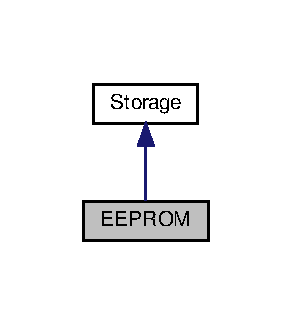
\includegraphics[width=140pt]{class_e_e_p_r_o_m__inherit__graph}
\end{center}
\end{figure}


Zusammengehörigkeiten von E\+E\+P\+R\+OM\+:\nopagebreak
\begin{figure}[H]
\begin{center}
\leavevmode
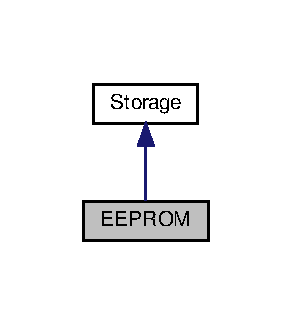
\includegraphics[width=140pt]{class_e_e_p_r_o_m__coll__graph}
\end{center}
\end{figure}
\subsection*{Öffentliche Methoden}
\begin{DoxyCompactItemize}
\item 
\textbf{ E\+E\+P\+R\+OM} (bool offline, string file\+Path)
\item 
virtual \textbf{ $\sim$\+E\+E\+P\+R\+OM} ()
\end{DoxyCompactItemize}
\subsection*{Weitere Geerbte Elemente}


\subsection{Beschreibung der Konstruktoren und Destruktoren}
\mbox{\label{class_e_e_p_r_o_m_a60c5bf54e6c1548bd2182a97d1c4cd09}} 
\index{E\+E\+P\+R\+OM@{E\+E\+P\+R\+OM}!E\+E\+P\+R\+OM@{E\+E\+P\+R\+OM}}
\index{E\+E\+P\+R\+OM@{E\+E\+P\+R\+OM}!E\+E\+P\+R\+OM@{E\+E\+P\+R\+OM}}
\subsubsection{E\+E\+P\+R\+O\+M()}
{\footnotesize\ttfamily E\+E\+P\+R\+O\+M\+::\+E\+E\+P\+R\+OM (\begin{DoxyParamCaption}\item[{bool}]{offline,  }\item[{string}]{file\+Path }\end{DoxyParamCaption})}

\mbox{\label{class_e_e_p_r_o_m_a8ed8926ed310a36b58940d9812829a97}} 
\index{E\+E\+P\+R\+OM@{E\+E\+P\+R\+OM}!````~E\+E\+P\+R\+OM@{$\sim$\+E\+E\+P\+R\+OM}}
\index{````~E\+E\+P\+R\+OM@{$\sim$\+E\+E\+P\+R\+OM}!E\+E\+P\+R\+OM@{E\+E\+P\+R\+OM}}
\subsubsection{$\sim$\+E\+E\+P\+R\+O\+M()}
{\footnotesize\ttfamily E\+E\+P\+R\+O\+M\+::$\sim$\+E\+E\+P\+R\+OM (\begin{DoxyParamCaption}{ }\end{DoxyParamCaption})\hspace{0.3cm}{\ttfamily [virtual]}}



Die Dokumentation für diese Klasse wurde erzeugt aufgrund der Dateien\+:\begin{DoxyCompactItemize}
\item 
/home/cjg8251/\+Desktop/\+Jura\+Coffee\+Memory/\textbf{ E\+E\+P\+R\+O\+M.\+hpp}\item 
/home/cjg8251/\+Desktop/\+Jura\+Coffee\+Memory/\textbf{ E\+E\+P\+R\+O\+M.\+cpp}\end{DoxyCompactItemize}

\section{E\+E\+P\+R\+O\+M\+\_\+\+Status Klassenreferenz}
\label{class_e_e_p_r_o_m___status}\index{E\+E\+P\+R\+O\+M\+\_\+\+Status@{E\+E\+P\+R\+O\+M\+\_\+\+Status}}


{\ttfamily \#include $<$E\+E\+P\+R\+O\+M\+\_\+\+Status.\+hpp$>$}



Klassendiagramm für E\+E\+P\+R\+O\+M\+\_\+\+Status\+:\nopagebreak
\begin{figure}[H]
\begin{center}
\leavevmode
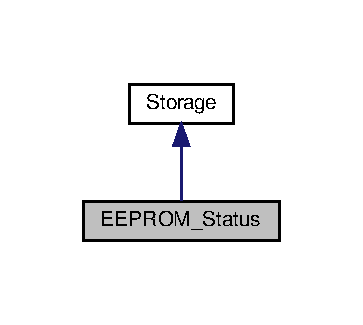
\includegraphics[width=174pt]{class_e_e_p_r_o_m___status__inherit__graph}
\end{center}
\end{figure}


Zusammengehörigkeiten von E\+E\+P\+R\+O\+M\+\_\+\+Status\+:\nopagebreak
\begin{figure}[H]
\begin{center}
\leavevmode
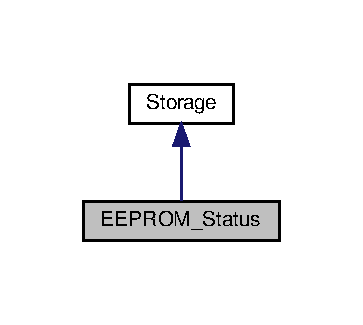
\includegraphics[width=174pt]{class_e_e_p_r_o_m___status__coll__graph}
\end{center}
\end{figure}
\subsection*{Öffentliche Methoden}
\begin{DoxyCompactItemize}
\item 
\textbf{ E\+E\+P\+R\+O\+M\+\_\+\+Status} ()
\item 
virtual \textbf{ $\sim$\+E\+E\+P\+R\+O\+M\+\_\+\+Status} ()
\item 
string \textbf{ get\+\_\+\+E\+E\+P\+R\+O\+M\+\_\+\+Status} ()
\item 
void \textbf{ pretty\+\_\+print\+\_\+json} ()
\item 
bool \textbf{ write\+\_\+\+E\+E\+P\+R\+OM} ()
\end{DoxyCompactItemize}
\subsection*{Weitere Geerbte Elemente}


\subsection{Beschreibung der Konstruktoren und Destruktoren}
\mbox{\label{class_e_e_p_r_o_m___status_ae5c247f1cba8c2409b9dbdb871c96b7b}} 
\index{E\+E\+P\+R\+O\+M\+\_\+\+Status@{E\+E\+P\+R\+O\+M\+\_\+\+Status}!E\+E\+P\+R\+O\+M\+\_\+\+Status@{E\+E\+P\+R\+O\+M\+\_\+\+Status}}
\index{E\+E\+P\+R\+O\+M\+\_\+\+Status@{E\+E\+P\+R\+O\+M\+\_\+\+Status}!E\+E\+P\+R\+O\+M\+\_\+\+Status@{E\+E\+P\+R\+O\+M\+\_\+\+Status}}
\subsubsection{E\+E\+P\+R\+O\+M\+\_\+\+Status()}
{\footnotesize\ttfamily E\+E\+P\+R\+O\+M\+\_\+\+Status\+::\+E\+E\+P\+R\+O\+M\+\_\+\+Status (\begin{DoxyParamCaption}{ }\end{DoxyParamCaption})}

\mbox{\label{class_e_e_p_r_o_m___status_a34a18e592fa670a1b92f98eb1a70c408}} 
\index{E\+E\+P\+R\+O\+M\+\_\+\+Status@{E\+E\+P\+R\+O\+M\+\_\+\+Status}!````~E\+E\+P\+R\+O\+M\+\_\+\+Status@{$\sim$\+E\+E\+P\+R\+O\+M\+\_\+\+Status}}
\index{````~E\+E\+P\+R\+O\+M\+\_\+\+Status@{$\sim$\+E\+E\+P\+R\+O\+M\+\_\+\+Status}!E\+E\+P\+R\+O\+M\+\_\+\+Status@{E\+E\+P\+R\+O\+M\+\_\+\+Status}}
\subsubsection{$\sim$\+E\+E\+P\+R\+O\+M\+\_\+\+Status()}
{\footnotesize\ttfamily E\+E\+P\+R\+O\+M\+\_\+\+Status\+::$\sim$\+E\+E\+P\+R\+O\+M\+\_\+\+Status (\begin{DoxyParamCaption}{ }\end{DoxyParamCaption})\hspace{0.3cm}{\ttfamily [virtual]}}

Hier ist ein Graph, der zeigt, was diese Funktion aufruft\+:
\nopagebreak
\begin{figure}[H]
\begin{center}
\leavevmode
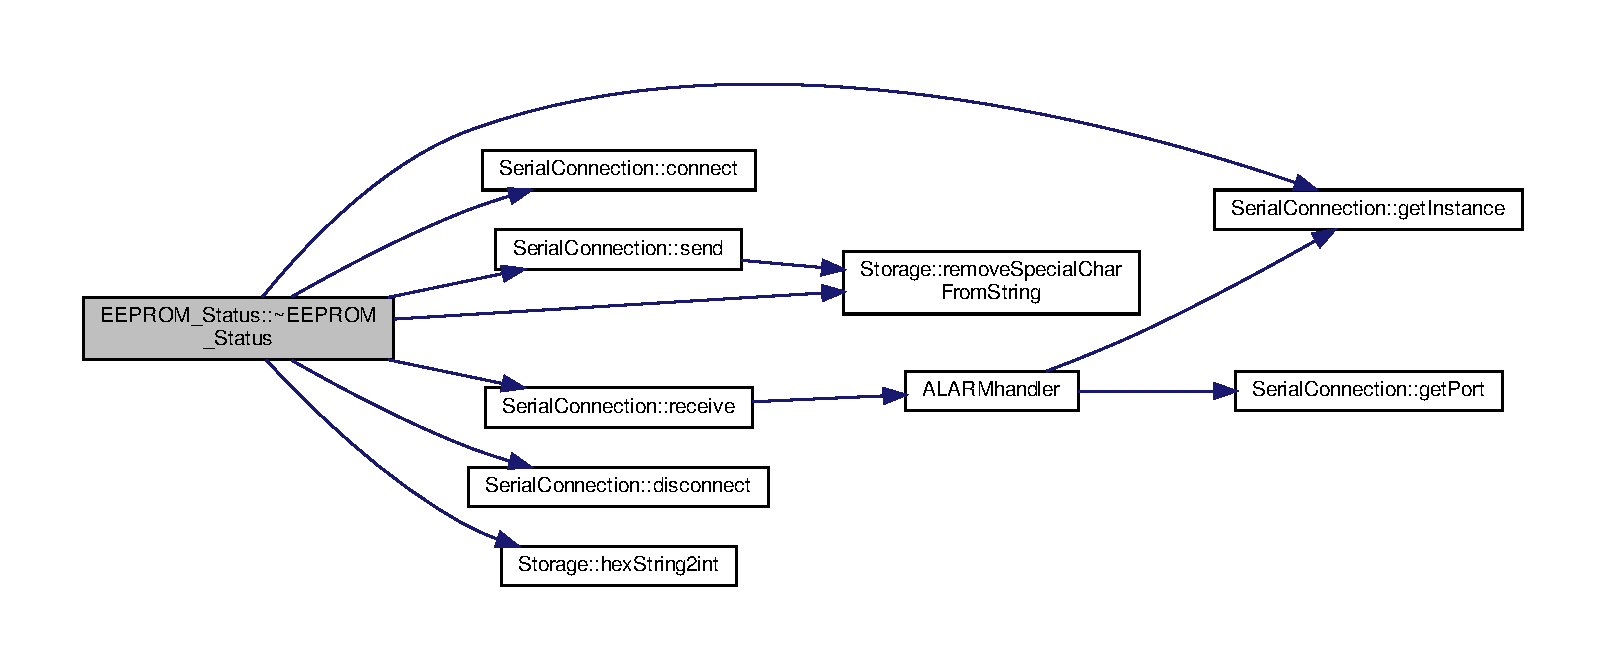
\includegraphics[width=350pt]{class_e_e_p_r_o_m___status_a34a18e592fa670a1b92f98eb1a70c408_cgraph}
\end{center}
\end{figure}


\subsection{Dokumentation der Elementfunktionen}
\mbox{\label{class_e_e_p_r_o_m___status_a8c4a7dd504e97e082bfd5b0399c89932}} 
\index{E\+E\+P\+R\+O\+M\+\_\+\+Status@{E\+E\+P\+R\+O\+M\+\_\+\+Status}!get\+\_\+\+E\+E\+P\+R\+O\+M\+\_\+\+Status@{get\+\_\+\+E\+E\+P\+R\+O\+M\+\_\+\+Status}}
\index{get\+\_\+\+E\+E\+P\+R\+O\+M\+\_\+\+Status@{get\+\_\+\+E\+E\+P\+R\+O\+M\+\_\+\+Status}!E\+E\+P\+R\+O\+M\+\_\+\+Status@{E\+E\+P\+R\+O\+M\+\_\+\+Status}}
\subsubsection{get\+\_\+\+E\+E\+P\+R\+O\+M\+\_\+\+Status()}
{\footnotesize\ttfamily string E\+E\+P\+R\+O\+M\+\_\+\+Status\+::get\+\_\+\+E\+E\+P\+R\+O\+M\+\_\+\+Status (\begin{DoxyParamCaption}{ }\end{DoxyParamCaption})}

\mbox{\label{class_e_e_p_r_o_m___status_a74969cfe2c7632e56b5ea69a3d3ac72a}} 
\index{E\+E\+P\+R\+O\+M\+\_\+\+Status@{E\+E\+P\+R\+O\+M\+\_\+\+Status}!pretty\+\_\+print\+\_\+json@{pretty\+\_\+print\+\_\+json}}
\index{pretty\+\_\+print\+\_\+json@{pretty\+\_\+print\+\_\+json}!E\+E\+P\+R\+O\+M\+\_\+\+Status@{E\+E\+P\+R\+O\+M\+\_\+\+Status}}
\subsubsection{pretty\+\_\+print\+\_\+json()}
{\footnotesize\ttfamily void E\+E\+P\+R\+O\+M\+\_\+\+Status\+::pretty\+\_\+print\+\_\+json (\begin{DoxyParamCaption}{ }\end{DoxyParamCaption})}

\mbox{\label{class_e_e_p_r_o_m___status_a090e971e61d1a15e76798b444240fd30}} 
\index{E\+E\+P\+R\+O\+M\+\_\+\+Status@{E\+E\+P\+R\+O\+M\+\_\+\+Status}!write\+\_\+\+E\+E\+P\+R\+OM@{write\+\_\+\+E\+E\+P\+R\+OM}}
\index{write\+\_\+\+E\+E\+P\+R\+OM@{write\+\_\+\+E\+E\+P\+R\+OM}!E\+E\+P\+R\+O\+M\+\_\+\+Status@{E\+E\+P\+R\+O\+M\+\_\+\+Status}}
\subsubsection{write\+\_\+\+E\+E\+P\+R\+O\+M()}
{\footnotesize\ttfamily bool E\+E\+P\+R\+O\+M\+\_\+\+Status\+::write\+\_\+\+E\+E\+P\+R\+OM (\begin{DoxyParamCaption}{ }\end{DoxyParamCaption})}

Hier ist ein Graph, der zeigt, was diese Funktion aufruft\+:
\nopagebreak
\begin{figure}[H]
\begin{center}
\leavevmode
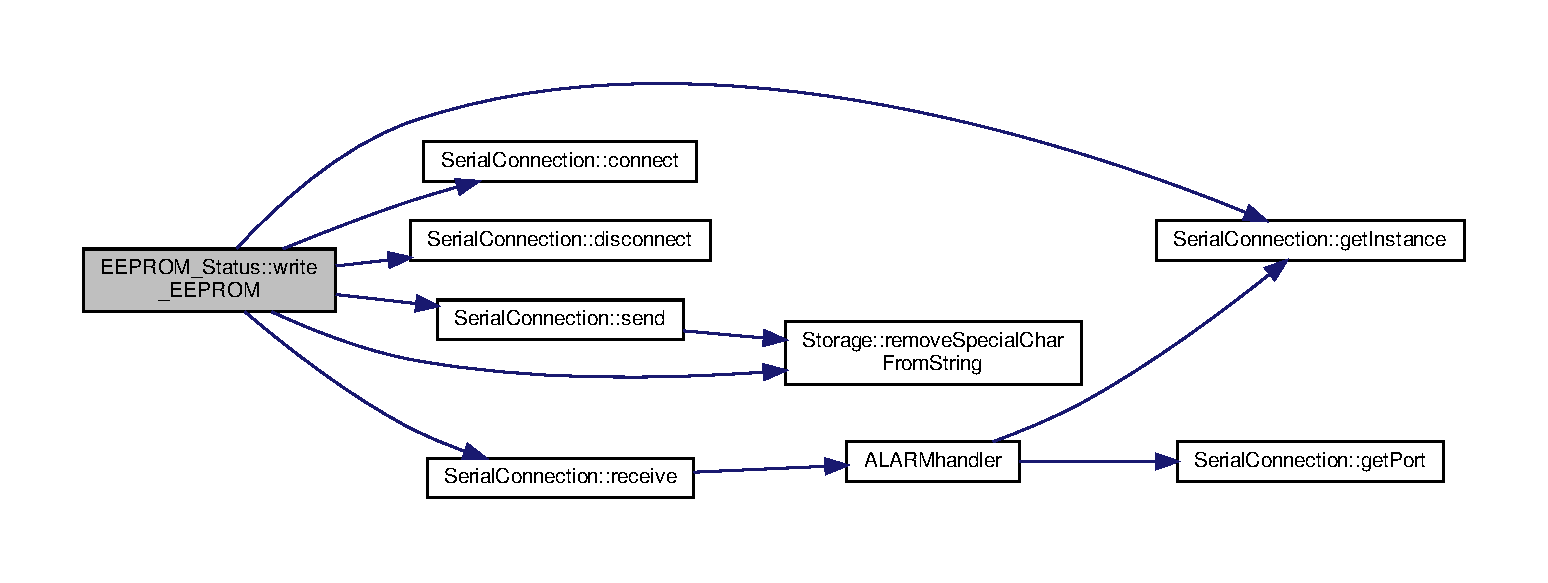
\includegraphics[width=350pt]{class_e_e_p_r_o_m___status_a090e971e61d1a15e76798b444240fd30_cgraph}
\end{center}
\end{figure}


Die Dokumentation für diese Klasse wurde erzeugt aufgrund der Dateien\+:\begin{DoxyCompactItemize}
\item 
/home/cjg8251/\+Desktop/\+Jura\+Coffee\+Memory/\textbf{ E\+E\+P\+R\+O\+M\+\_\+\+Status.\+hpp}\item 
/home/cjg8251/\+Desktop/\+Jura\+Coffee\+Memory/\textbf{ E\+E\+P\+R\+O\+M\+\_\+\+Status.\+cpp}\end{DoxyCompactItemize}

\section{Entry\+E\+E\+P\+R\+OM Strukturreferenz}
\label{struct_entry_e_e_p_r_o_m}\index{Entry\+E\+E\+P\+R\+OM@{Entry\+E\+E\+P\+R\+OM}}


{\ttfamily \#include $<$E\+E\+P\+R\+O\+M\+\_\+\+Status.\+hpp$>$}

\subsection*{Öffentliche Methoden}
\begin{DoxyCompactItemize}
\item 
bool \textbf{ operator$<$} (const \textbf{ Entry\+E\+E\+P\+R\+OM} \&other) const
\end{DoxyCompactItemize}
\subsection*{Öffentliche Attribute}
\begin{DoxyCompactItemize}
\item 
int \textbf{ word}
\item 
set$<$ int $>$ \textbf{ bytes}
\item 
string \textbf{ label}
\end{DoxyCompactItemize}


\subsection{Dokumentation der Elementfunktionen}
\mbox{\label{struct_entry_e_e_p_r_o_m_ad338c7f94d5ed103e07d6090395cf381}} 
\index{Entry\+E\+E\+P\+R\+OM@{Entry\+E\+E\+P\+R\+OM}!operator$<$@{operator$<$}}
\index{operator$<$@{operator$<$}!Entry\+E\+E\+P\+R\+OM@{Entry\+E\+E\+P\+R\+OM}}
\subsubsection{operator$<$()}
{\footnotesize\ttfamily bool Entry\+E\+E\+P\+R\+O\+M\+::operator$<$ (\begin{DoxyParamCaption}\item[{const \textbf{ Entry\+E\+E\+P\+R\+OM} \&}]{other }\end{DoxyParamCaption}) const\hspace{0.3cm}{\ttfamily [inline]}}



\subsection{Dokumentation der Datenelemente}
\mbox{\label{struct_entry_e_e_p_r_o_m_a5286fd447a14070a11278d2db28c122e}} 
\index{Entry\+E\+E\+P\+R\+OM@{Entry\+E\+E\+P\+R\+OM}!bytes@{bytes}}
\index{bytes@{bytes}!Entry\+E\+E\+P\+R\+OM@{Entry\+E\+E\+P\+R\+OM}}
\subsubsection{bytes}
{\footnotesize\ttfamily set$<$int$>$ Entry\+E\+E\+P\+R\+O\+M\+::bytes}

\mbox{\label{struct_entry_e_e_p_r_o_m_abdba61f5a81a7b4d99159271ef11df3b}} 
\index{Entry\+E\+E\+P\+R\+OM@{Entry\+E\+E\+P\+R\+OM}!label@{label}}
\index{label@{label}!Entry\+E\+E\+P\+R\+OM@{Entry\+E\+E\+P\+R\+OM}}
\subsubsection{label}
{\footnotesize\ttfamily string Entry\+E\+E\+P\+R\+O\+M\+::label}

\mbox{\label{struct_entry_e_e_p_r_o_m_a183abe74905c3ff64dec46b7c322527f}} 
\index{Entry\+E\+E\+P\+R\+OM@{Entry\+E\+E\+P\+R\+OM}!word@{word}}
\index{word@{word}!Entry\+E\+E\+P\+R\+OM@{Entry\+E\+E\+P\+R\+OM}}
\subsubsection{word}
{\footnotesize\ttfamily int Entry\+E\+E\+P\+R\+O\+M\+::word}



Die Dokumentation für diese Struktur wurde erzeugt aufgrund der Datei\+:\begin{DoxyCompactItemize}
\item 
/home/cjg8251/\+Desktop/\+Jura\+Coffee\+Memory/\textbf{ E\+E\+P\+R\+O\+M\+\_\+\+Status.\+hpp}\end{DoxyCompactItemize}

\section{Entry\+R\+AM Strukturreferenz}
\label{struct_entry_r_a_m}\index{Entry\+R\+AM@{Entry\+R\+AM}}


{\ttfamily \#include $<$R\+A\+M\+\_\+\+Status.\+hpp$>$}

\subsection*{Öffentliche Methoden}
\begin{DoxyCompactItemize}
\item 
bool \textbf{ operator$<$} (const \textbf{ Entry\+R\+AM} \&other) const
\end{DoxyCompactItemize}
\subsection*{Öffentliche Attribute}
\begin{DoxyCompactItemize}
\item 
int \textbf{ byte}
\item 
set$<$ int $>$ \textbf{ bits}
\item 
string \textbf{ label}
\end{DoxyCompactItemize}


\subsection{Dokumentation der Elementfunktionen}
\mbox{\label{struct_entry_r_a_m_a301882e799b70aebc8eae3bb55ba253a}} 
\index{Entry\+R\+AM@{Entry\+R\+AM}!operator$<$@{operator$<$}}
\index{operator$<$@{operator$<$}!Entry\+R\+AM@{Entry\+R\+AM}}
\subsubsection{operator$<$()}
{\footnotesize\ttfamily bool Entry\+R\+A\+M\+::operator$<$ (\begin{DoxyParamCaption}\item[{const \textbf{ Entry\+R\+AM} \&}]{other }\end{DoxyParamCaption}) const\hspace{0.3cm}{\ttfamily [inline]}}



\subsection{Dokumentation der Datenelemente}
\mbox{\label{struct_entry_r_a_m_adf440ec20cd0f00c8f51c7ce3621e403}} 
\index{Entry\+R\+AM@{Entry\+R\+AM}!bits@{bits}}
\index{bits@{bits}!Entry\+R\+AM@{Entry\+R\+AM}}
\subsubsection{bits}
{\footnotesize\ttfamily set$<$int$>$ Entry\+R\+A\+M\+::bits}

\mbox{\label{struct_entry_r_a_m_a6c05b2b828a93b2f5e75ffc4c0b8d223}} 
\index{Entry\+R\+AM@{Entry\+R\+AM}!byte@{byte}}
\index{byte@{byte}!Entry\+R\+AM@{Entry\+R\+AM}}
\subsubsection{byte}
{\footnotesize\ttfamily int Entry\+R\+A\+M\+::byte}

\mbox{\label{struct_entry_r_a_m_a7e464f0594a4f376d163f6dc17a00e5b}} 
\index{Entry\+R\+AM@{Entry\+R\+AM}!label@{label}}
\index{label@{label}!Entry\+R\+AM@{Entry\+R\+AM}}
\subsubsection{label}
{\footnotesize\ttfamily string Entry\+R\+A\+M\+::label}



Die Dokumentation für diese Struktur wurde erzeugt aufgrund der Datei\+:\begin{DoxyCompactItemize}
\item 
/home/cjg8251/\+Desktop/\+Jura\+Coffee\+Memory/\textbf{ R\+A\+M\+\_\+\+Status.\+hpp}\end{DoxyCompactItemize}

\section{Json\+File Klassenreferenz}
\label{class_json_file}\index{Json\+File@{Json\+File}}


{\ttfamily \#include $<$Json\+File.\+hpp$>$}

\subsection*{Öffentliche Methoden}
\begin{DoxyCompactItemize}
\item 
virtual \textbf{ $\sim$\+Json\+File} ()
\item 
Json\+::\+Value \textbf{ read\+Json} (string file\+Path)
\item 
void \textbf{ log\+Data} (string file\+Path, int i, string s)
\item 
void \textbf{ log\+Raw\+Data} (string file\+Path, string raw\+Old, string raw\+New, string comment)
\item 
vector$<$ \textbf{ dump} $>$ \textbf{ get\+Dumps} ()
\item 
vector$<$ \textbf{ data} $>$ \textbf{ get\+Data} ()
\end{DoxyCompactItemize}
\subsection*{Öffentliche, statische Methoden}
\begin{DoxyCompactItemize}
\item 
static \textbf{ Json\+File} \& \textbf{ get\+Instance} ()
\end{DoxyCompactItemize}


\subsection{Beschreibung der Konstruktoren und Destruktoren}
\mbox{\label{class_json_file_a3a821a767cdf009865b519527731a007}} 
\index{Json\+File@{Json\+File}!````~Json\+File@{$\sim$\+Json\+File}}
\index{````~Json\+File@{$\sim$\+Json\+File}!Json\+File@{Json\+File}}
\subsubsection{$\sim$\+Json\+File()}
{\footnotesize\ttfamily Json\+File\+::$\sim$\+Json\+File (\begin{DoxyParamCaption}{ }\end{DoxyParamCaption})\hspace{0.3cm}{\ttfamily [virtual]}}



\subsection{Dokumentation der Elementfunktionen}
\mbox{\label{class_json_file_a5920a87442b0f6250e3013362d10b0b5}} 
\index{Json\+File@{Json\+File}!get\+Data@{get\+Data}}
\index{get\+Data@{get\+Data}!Json\+File@{Json\+File}}
\subsubsection{get\+Data()}
{\footnotesize\ttfamily vector$<$ \textbf{ data} $>$ Json\+File\+::get\+Data (\begin{DoxyParamCaption}{ }\end{DoxyParamCaption})}

\mbox{\label{class_json_file_a973aa4aba725db652ddb6edd26ff8527}} 
\index{Json\+File@{Json\+File}!get\+Dumps@{get\+Dumps}}
\index{get\+Dumps@{get\+Dumps}!Json\+File@{Json\+File}}
\subsubsection{get\+Dumps()}
{\footnotesize\ttfamily vector$<$ \textbf{ dump} $>$ Json\+File\+::get\+Dumps (\begin{DoxyParamCaption}{ }\end{DoxyParamCaption})}

\mbox{\label{class_json_file_a70ea731be6e00b083190c011e0ee4392}} 
\index{Json\+File@{Json\+File}!get\+Instance@{get\+Instance}}
\index{get\+Instance@{get\+Instance}!Json\+File@{Json\+File}}
\subsubsection{get\+Instance()}
{\footnotesize\ttfamily \textbf{ Json\+File} \& Json\+File\+::get\+Instance (\begin{DoxyParamCaption}{ }\end{DoxyParamCaption})\hspace{0.3cm}{\ttfamily [static]}}

\mbox{\label{class_json_file_a69c66d052ccb40a11396f537787a6343}} 
\index{Json\+File@{Json\+File}!log\+Data@{log\+Data}}
\index{log\+Data@{log\+Data}!Json\+File@{Json\+File}}
\subsubsection{log\+Data()}
{\footnotesize\ttfamily void Json\+File\+::log\+Data (\begin{DoxyParamCaption}\item[{string}]{file\+Path,  }\item[{int}]{i,  }\item[{string}]{s }\end{DoxyParamCaption})}

Hier ist ein Graph, der zeigt, was diese Funktion aufruft\+:\nopagebreak
\begin{figure}[H]
\begin{center}
\leavevmode
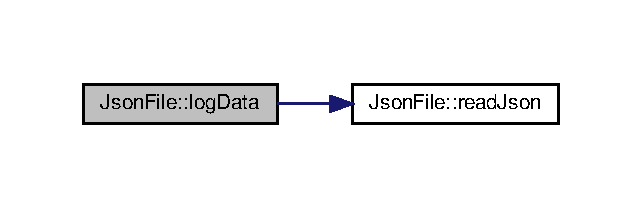
\includegraphics[width=308pt]{class_json_file_a69c66d052ccb40a11396f537787a6343_cgraph}
\end{center}
\end{figure}
\mbox{\label{class_json_file_a8361a5de646f07365b7baeae80f6d3eb}} 
\index{Json\+File@{Json\+File}!log\+Raw\+Data@{log\+Raw\+Data}}
\index{log\+Raw\+Data@{log\+Raw\+Data}!Json\+File@{Json\+File}}
\subsubsection{log\+Raw\+Data()}
{\footnotesize\ttfamily void Json\+File\+::log\+Raw\+Data (\begin{DoxyParamCaption}\item[{string}]{file\+Path,  }\item[{string}]{raw\+Old,  }\item[{string}]{raw\+New,  }\item[{string}]{comment }\end{DoxyParamCaption})}

Hier ist ein Graph, der zeigt, was diese Funktion aufruft\+:\nopagebreak
\begin{figure}[H]
\begin{center}
\leavevmode
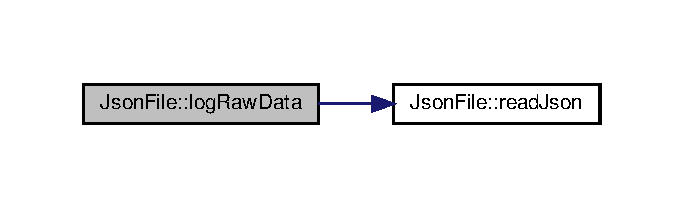
\includegraphics[width=328pt]{class_json_file_a8361a5de646f07365b7baeae80f6d3eb_cgraph}
\end{center}
\end{figure}
\mbox{\label{class_json_file_a0b7eb46810847ba22ea137a4ce4757ae}} 
\index{Json\+File@{Json\+File}!read\+Json@{read\+Json}}
\index{read\+Json@{read\+Json}!Json\+File@{Json\+File}}
\subsubsection{read\+Json()}
{\footnotesize\ttfamily Json\+::\+Value Json\+File\+::read\+Json (\begin{DoxyParamCaption}\item[{string}]{file\+Path }\end{DoxyParamCaption})}



Die Dokumentation für diese Klasse wurde erzeugt aufgrund der Dateien\+:\begin{DoxyCompactItemize}
\item 
/home/cjg8251/\+Desktop/\+Jura\+Coffee\+Memory/\textbf{ Json\+File.\+hpp}\item 
/home/cjg8251/\+Desktop/\+Jura\+Coffee\+Memory/\textbf{ Json\+File.\+cpp}\end{DoxyCompactItemize}

\section{R\+AM Klassenreferenz}
\label{class_r_a_m}\index{R\+AM@{R\+AM}}


{\ttfamily \#include $<$R\+A\+M.\+hpp$>$}



Klassendiagramm für R\+AM\+:\nopagebreak
\begin{figure}[H]
\begin{center}
\leavevmode
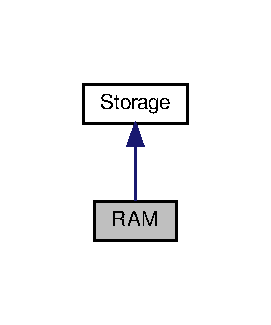
\includegraphics[width=130pt]{class_r_a_m__inherit__graph}
\end{center}
\end{figure}


Zusammengehörigkeiten von R\+AM\+:\nopagebreak
\begin{figure}[H]
\begin{center}
\leavevmode
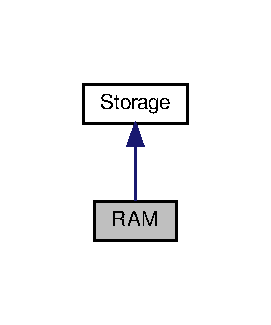
\includegraphics[width=130pt]{class_r_a_m__coll__graph}
\end{center}
\end{figure}
\subsection*{Öffentliche Methoden}
\begin{DoxyCompactItemize}
\item 
\textbf{ R\+AM} (bool offline, string file\+Path)
\item 
virtual \textbf{ $\sim$\+R\+AM} ()
\end{DoxyCompactItemize}
\subsection*{Weitere Geerbte Elemente}


\subsection{Beschreibung der Konstruktoren und Destruktoren}
\mbox{\label{class_r_a_m_ad922e92719a50987d398e771cf8cf88b}} 
\index{R\+AM@{R\+AM}!R\+AM@{R\+AM}}
\index{R\+AM@{R\+AM}!R\+AM@{R\+AM}}
\subsubsection{R\+A\+M()}
{\footnotesize\ttfamily R\+A\+M\+::\+R\+AM (\begin{DoxyParamCaption}\item[{bool}]{offline,  }\item[{string}]{file\+Path }\end{DoxyParamCaption})}

\mbox{\label{class_r_a_m_ac884b3e9ee3c3d95ebcd7b6ed9851da3}} 
\index{R\+AM@{R\+AM}!````~R\+AM@{$\sim$\+R\+AM}}
\index{````~R\+AM@{$\sim$\+R\+AM}!R\+AM@{R\+AM}}
\subsubsection{$\sim$\+R\+A\+M()}
{\footnotesize\ttfamily R\+A\+M\+::$\sim$\+R\+AM (\begin{DoxyParamCaption}{ }\end{DoxyParamCaption})\hspace{0.3cm}{\ttfamily [virtual]}}



Die Dokumentation für diese Klasse wurde erzeugt aufgrund der Dateien\+:\begin{DoxyCompactItemize}
\item 
/home/cjg8251/\+Desktop/\+Jura\+Coffee\+Memory/\textbf{ R\+A\+M.\+hpp}\item 
/home/cjg8251/\+Desktop/\+Jura\+Coffee\+Memory/\textbf{ R\+A\+M.\+cpp}\end{DoxyCompactItemize}

\section{R\+A\+M\+\_\+\+Status Klassenreferenz}
\label{class_r_a_m___status}\index{R\+A\+M\+\_\+\+Status@{R\+A\+M\+\_\+\+Status}}


{\ttfamily \#include $<$R\+A\+M\+\_\+\+Status.\+hpp$>$}



Klassendiagramm für R\+A\+M\+\_\+\+Status\+:\nopagebreak
\begin{figure}[H]
\begin{center}
\leavevmode
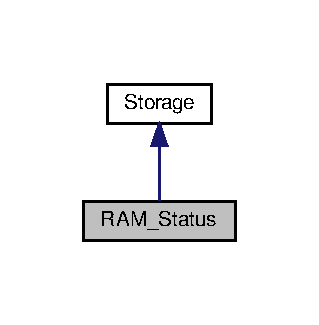
\includegraphics[width=153pt]{class_r_a_m___status__inherit__graph}
\end{center}
\end{figure}


Zusammengehörigkeiten von R\+A\+M\+\_\+\+Status\+:\nopagebreak
\begin{figure}[H]
\begin{center}
\leavevmode
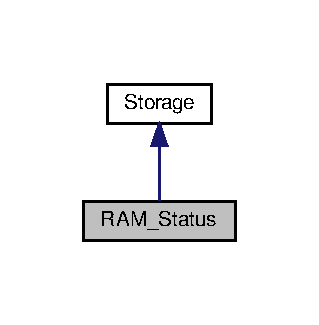
\includegraphics[width=153pt]{class_r_a_m___status__coll__graph}
\end{center}
\end{figure}
\subsection*{Öffentliche Methoden}
\begin{DoxyCompactItemize}
\item 
\textbf{ R\+A\+M\+\_\+\+Status} ()
\item 
virtual \textbf{ $\sim$\+R\+A\+M\+\_\+\+Status} ()
\item 
string \textbf{ get\+\_\+\+R\+A\+M\+\_\+\+Status} ()
\item 
void \textbf{ pretty\+\_\+print\+\_\+json} ()
\end{DoxyCompactItemize}
\subsection*{Weitere Geerbte Elemente}


\subsection{Beschreibung der Konstruktoren und Destruktoren}
\mbox{\label{class_r_a_m___status_a66e7668bfd1949beceb2a4c3ebc2aaaa}} 
\index{R\+A\+M\+\_\+\+Status@{R\+A\+M\+\_\+\+Status}!R\+A\+M\+\_\+\+Status@{R\+A\+M\+\_\+\+Status}}
\index{R\+A\+M\+\_\+\+Status@{R\+A\+M\+\_\+\+Status}!R\+A\+M\+\_\+\+Status@{R\+A\+M\+\_\+\+Status}}
\subsubsection{R\+A\+M\+\_\+\+Status()}
{\footnotesize\ttfamily R\+A\+M\+\_\+\+Status\+::\+R\+A\+M\+\_\+\+Status (\begin{DoxyParamCaption}{ }\end{DoxyParamCaption})}

\mbox{\label{class_r_a_m___status_ae0f0b32a57c9f02553f22abd6e49fbba}} 
\index{R\+A\+M\+\_\+\+Status@{R\+A\+M\+\_\+\+Status}!````~R\+A\+M\+\_\+\+Status@{$\sim$\+R\+A\+M\+\_\+\+Status}}
\index{````~R\+A\+M\+\_\+\+Status@{$\sim$\+R\+A\+M\+\_\+\+Status}!R\+A\+M\+\_\+\+Status@{R\+A\+M\+\_\+\+Status}}
\subsubsection{$\sim$\+R\+A\+M\+\_\+\+Status()}
{\footnotesize\ttfamily R\+A\+M\+\_\+\+Status\+::$\sim$\+R\+A\+M\+\_\+\+Status (\begin{DoxyParamCaption}{ }\end{DoxyParamCaption})\hspace{0.3cm}{\ttfamily [virtual]}}

Hier ist ein Graph, der zeigt, was diese Funktion aufruft\+:
\nopagebreak
\begin{figure}[H]
\begin{center}
\leavevmode
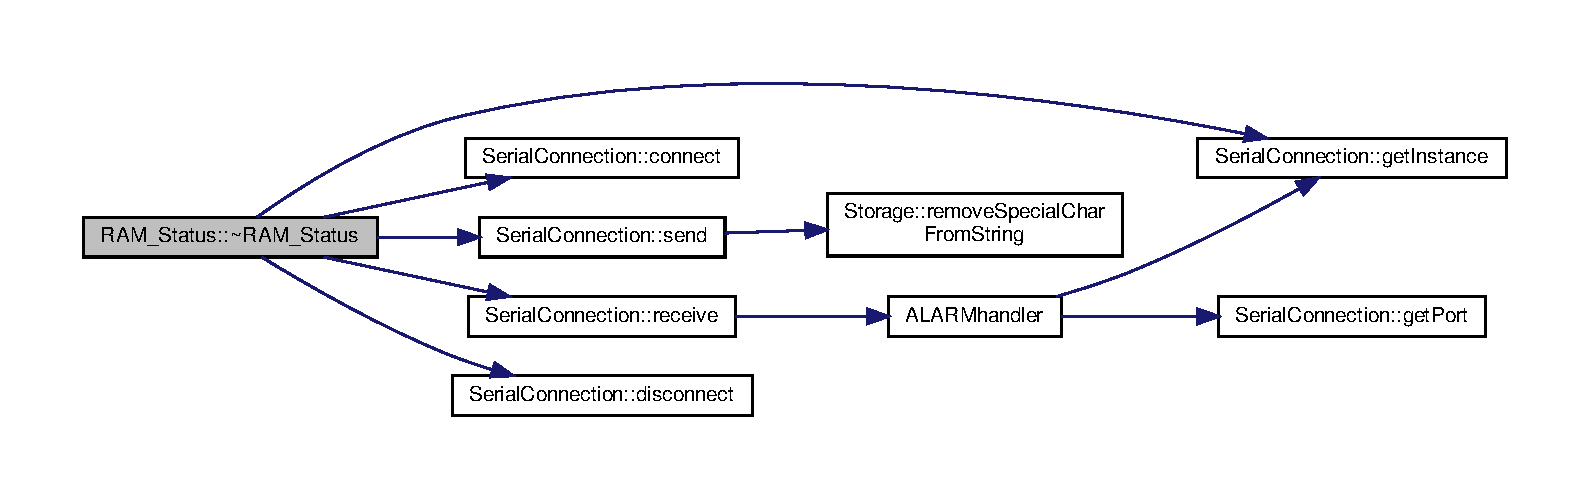
\includegraphics[width=350pt]{class_r_a_m___status_ae0f0b32a57c9f02553f22abd6e49fbba_cgraph}
\end{center}
\end{figure}


\subsection{Dokumentation der Elementfunktionen}
\mbox{\label{class_r_a_m___status_aa4e4c37f9eecaa92dbf6ab6805fba5fc}} 
\index{R\+A\+M\+\_\+\+Status@{R\+A\+M\+\_\+\+Status}!get\+\_\+\+R\+A\+M\+\_\+\+Status@{get\+\_\+\+R\+A\+M\+\_\+\+Status}}
\index{get\+\_\+\+R\+A\+M\+\_\+\+Status@{get\+\_\+\+R\+A\+M\+\_\+\+Status}!R\+A\+M\+\_\+\+Status@{R\+A\+M\+\_\+\+Status}}
\subsubsection{get\+\_\+\+R\+A\+M\+\_\+\+Status()}
{\footnotesize\ttfamily string R\+A\+M\+\_\+\+Status\+::get\+\_\+\+R\+A\+M\+\_\+\+Status (\begin{DoxyParamCaption}{ }\end{DoxyParamCaption})}

\mbox{\label{class_r_a_m___status_a098ae3e77c3185c33852f0d3c621af4f}} 
\index{R\+A\+M\+\_\+\+Status@{R\+A\+M\+\_\+\+Status}!pretty\+\_\+print\+\_\+json@{pretty\+\_\+print\+\_\+json}}
\index{pretty\+\_\+print\+\_\+json@{pretty\+\_\+print\+\_\+json}!R\+A\+M\+\_\+\+Status@{R\+A\+M\+\_\+\+Status}}
\subsubsection{pretty\+\_\+print\+\_\+json()}
{\footnotesize\ttfamily void R\+A\+M\+\_\+\+Status\+::pretty\+\_\+print\+\_\+json (\begin{DoxyParamCaption}{ }\end{DoxyParamCaption})}



Die Dokumentation für diese Klasse wurde erzeugt aufgrund der Dateien\+:\begin{DoxyCompactItemize}
\item 
/home/cjg8251/\+Desktop/\+Jura\+Coffee\+Memory/\textbf{ R\+A\+M\+\_\+\+Status.\+hpp}\item 
/home/cjg8251/\+Desktop/\+Jura\+Coffee\+Memory/\textbf{ R\+A\+M\+\_\+\+Status.\+cpp}\end{DoxyCompactItemize}

\section{Serial\+Connection Klassenreferenz}
\label{class_serial_connection}\index{Serial\+Connection@{Serial\+Connection}}


{\ttfamily \#include $<$Serial\+Connection.\+hpp$>$}

\subsection*{Öffentliche Methoden}
\begin{DoxyCompactItemize}
\item 
virtual \textbf{ $\sim$\+Serial\+Connection} ()
\item 
void \textbf{ set\+Port} (string port)
\item 
string \textbf{ get\+Port} ()
\item 
void \textbf{ set\+Command\+Suffix} (string suffix)
\item 
string \textbf{ get\+Command\+Suffix} ()
\item 
void \textbf{ connect} ()
\item 
void \textbf{ disconnect} ()
\item 
bool \textbf{ test\+Connection} ()
\item 
void \textbf{ set\+Test\+Command} (string command)
\item 
string \textbf{ get\+Test\+Command} ()
\item 
void \textbf{ set\+Test\+Answer} (string answer)
\item 
string \textbf{ get\+Test\+Answer} ()
\item 
void \textbf{ send} (string txt)
\item 
string \textbf{ receive} ()
\end{DoxyCompactItemize}
\subsection*{Öffentliche, statische Methoden}
\begin{DoxyCompactItemize}
\item 
static \textbf{ Serial\+Connection} \& \textbf{ get\+Instance} ()
\end{DoxyCompactItemize}
\subsection*{Öffentliche Attribute}
\begin{DoxyCompactItemize}
\item 
string \textbf{ test\+Command}
\item 
string \textbf{ test\+Answer}
\end{DoxyCompactItemize}


\subsection{Beschreibung der Konstruktoren und Destruktoren}
\mbox{\label{class_serial_connection_ae73749bb08c2f53f467809cb6c0a3fc8}} 
\index{Serial\+Connection@{Serial\+Connection}!````~Serial\+Connection@{$\sim$\+Serial\+Connection}}
\index{````~Serial\+Connection@{$\sim$\+Serial\+Connection}!Serial\+Connection@{Serial\+Connection}}
\subsubsection{$\sim$\+Serial\+Connection()}
{\footnotesize\ttfamily Serial\+Connection\+::$\sim$\+Serial\+Connection (\begin{DoxyParamCaption}{ }\end{DoxyParamCaption})\hspace{0.3cm}{\ttfamily [virtual]}}



\subsection{Dokumentation der Elementfunktionen}
\mbox{\label{class_serial_connection_a6b1e786b3d6cc46d744f780284f24402}} 
\index{Serial\+Connection@{Serial\+Connection}!connect@{connect}}
\index{connect@{connect}!Serial\+Connection@{Serial\+Connection}}
\subsubsection{connect()}
{\footnotesize\ttfamily void Serial\+Connection\+::connect (\begin{DoxyParamCaption}{ }\end{DoxyParamCaption})}

\mbox{\label{class_serial_connection_a395259938f38535125f070b8ac00719d}} 
\index{Serial\+Connection@{Serial\+Connection}!disconnect@{disconnect}}
\index{disconnect@{disconnect}!Serial\+Connection@{Serial\+Connection}}
\subsubsection{disconnect()}
{\footnotesize\ttfamily void Serial\+Connection\+::disconnect (\begin{DoxyParamCaption}{ }\end{DoxyParamCaption})}

\mbox{\label{class_serial_connection_a85bda71650f96501c4142347d2fd45ea}} 
\index{Serial\+Connection@{Serial\+Connection}!get\+Command\+Suffix@{get\+Command\+Suffix}}
\index{get\+Command\+Suffix@{get\+Command\+Suffix}!Serial\+Connection@{Serial\+Connection}}
\subsubsection{get\+Command\+Suffix()}
{\footnotesize\ttfamily string Serial\+Connection\+::get\+Command\+Suffix (\begin{DoxyParamCaption}{ }\end{DoxyParamCaption})}

\mbox{\label{class_serial_connection_ac98b98a509727eb43dd4e09a9bc47eb8}} 
\index{Serial\+Connection@{Serial\+Connection}!get\+Instance@{get\+Instance}}
\index{get\+Instance@{get\+Instance}!Serial\+Connection@{Serial\+Connection}}
\subsubsection{get\+Instance()}
{\footnotesize\ttfamily \textbf{ Serial\+Connection} \& Serial\+Connection\+::get\+Instance (\begin{DoxyParamCaption}{ }\end{DoxyParamCaption})\hspace{0.3cm}{\ttfamily [static]}}

\mbox{\label{class_serial_connection_a2ecb1ba029fefbc9697262e9f9cb5e5b}} 
\index{Serial\+Connection@{Serial\+Connection}!get\+Port@{get\+Port}}
\index{get\+Port@{get\+Port}!Serial\+Connection@{Serial\+Connection}}
\subsubsection{get\+Port()}
{\footnotesize\ttfamily string Serial\+Connection\+::get\+Port (\begin{DoxyParamCaption}{ }\end{DoxyParamCaption})}

\mbox{\label{class_serial_connection_a9fb2b43e439ec8b3d00aa4be0c51bcc6}} 
\index{Serial\+Connection@{Serial\+Connection}!get\+Test\+Answer@{get\+Test\+Answer}}
\index{get\+Test\+Answer@{get\+Test\+Answer}!Serial\+Connection@{Serial\+Connection}}
\subsubsection{get\+Test\+Answer()}
{\footnotesize\ttfamily string Serial\+Connection\+::get\+Test\+Answer (\begin{DoxyParamCaption}{ }\end{DoxyParamCaption})}

\mbox{\label{class_serial_connection_a254f0b760e29c3584a0e8b55601b4bc6}} 
\index{Serial\+Connection@{Serial\+Connection}!get\+Test\+Command@{get\+Test\+Command}}
\index{get\+Test\+Command@{get\+Test\+Command}!Serial\+Connection@{Serial\+Connection}}
\subsubsection{get\+Test\+Command()}
{\footnotesize\ttfamily string Serial\+Connection\+::get\+Test\+Command (\begin{DoxyParamCaption}{ }\end{DoxyParamCaption})}

\mbox{\label{class_serial_connection_a6419c43953bb392053479353420a1f8e}} 
\index{Serial\+Connection@{Serial\+Connection}!receive@{receive}}
\index{receive@{receive}!Serial\+Connection@{Serial\+Connection}}
\subsubsection{receive()}
{\footnotesize\ttfamily string Serial\+Connection\+::receive (\begin{DoxyParamCaption}{ }\end{DoxyParamCaption})}

Hier ist ein Graph, der zeigt, was diese Funktion aufruft\+:\nopagebreak
\begin{figure}[H]
\begin{center}
\leavevmode
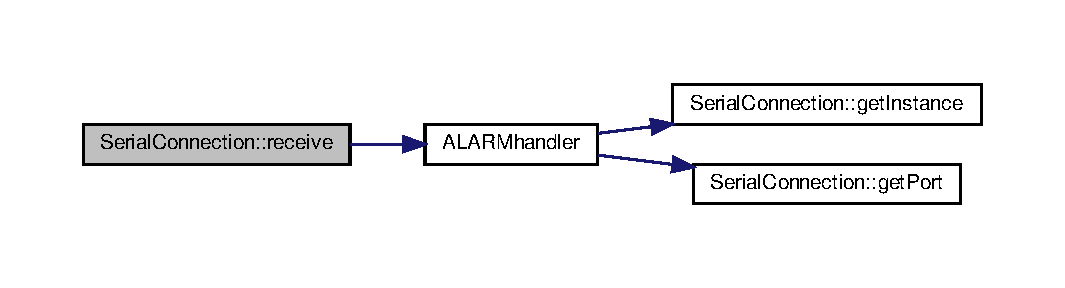
\includegraphics[width=350pt]{class_serial_connection_a6419c43953bb392053479353420a1f8e_cgraph}
\end{center}
\end{figure}
\mbox{\label{class_serial_connection_a31a09de5479fb612aac94ade315d6f0e}} 
\index{Serial\+Connection@{Serial\+Connection}!send@{send}}
\index{send@{send}!Serial\+Connection@{Serial\+Connection}}
\subsubsection{send()}
{\footnotesize\ttfamily void Serial\+Connection\+::send (\begin{DoxyParamCaption}\item[{string}]{txt }\end{DoxyParamCaption})}

Hier ist ein Graph, der zeigt, was diese Funktion aufruft\+:\nopagebreak
\begin{figure}[H]
\begin{center}
\leavevmode
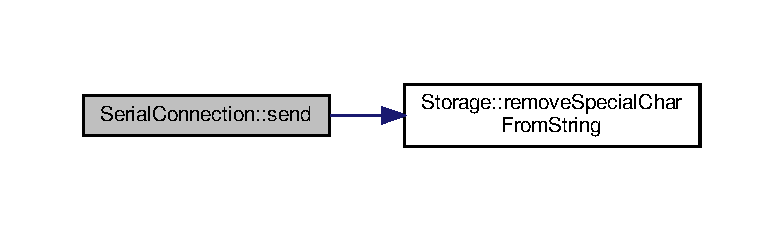
\includegraphics[width=350pt]{class_serial_connection_a31a09de5479fb612aac94ade315d6f0e_cgraph}
\end{center}
\end{figure}
\mbox{\label{class_serial_connection_aee2098908b7fcdc959c4029f6cf02151}} 
\index{Serial\+Connection@{Serial\+Connection}!set\+Command\+Suffix@{set\+Command\+Suffix}}
\index{set\+Command\+Suffix@{set\+Command\+Suffix}!Serial\+Connection@{Serial\+Connection}}
\subsubsection{set\+Command\+Suffix()}
{\footnotesize\ttfamily void Serial\+Connection\+::set\+Command\+Suffix (\begin{DoxyParamCaption}\item[{string}]{suffix }\end{DoxyParamCaption})}

\mbox{\label{class_serial_connection_af12096e43282f0857d05ad7f4c26e655}} 
\index{Serial\+Connection@{Serial\+Connection}!set\+Port@{set\+Port}}
\index{set\+Port@{set\+Port}!Serial\+Connection@{Serial\+Connection}}
\subsubsection{set\+Port()}
{\footnotesize\ttfamily void Serial\+Connection\+::set\+Port (\begin{DoxyParamCaption}\item[{string}]{port }\end{DoxyParamCaption})}

\mbox{\label{class_serial_connection_aadcb81bf3f4f3e90676b5c9495ea497f}} 
\index{Serial\+Connection@{Serial\+Connection}!set\+Test\+Answer@{set\+Test\+Answer}}
\index{set\+Test\+Answer@{set\+Test\+Answer}!Serial\+Connection@{Serial\+Connection}}
\subsubsection{set\+Test\+Answer()}
{\footnotesize\ttfamily void Serial\+Connection\+::set\+Test\+Answer (\begin{DoxyParamCaption}\item[{string}]{answer }\end{DoxyParamCaption})}

\mbox{\label{class_serial_connection_a9672748d2a2e36a6e4798a63fb91deff}} 
\index{Serial\+Connection@{Serial\+Connection}!set\+Test\+Command@{set\+Test\+Command}}
\index{set\+Test\+Command@{set\+Test\+Command}!Serial\+Connection@{Serial\+Connection}}
\subsubsection{set\+Test\+Command()}
{\footnotesize\ttfamily void Serial\+Connection\+::set\+Test\+Command (\begin{DoxyParamCaption}\item[{string}]{command }\end{DoxyParamCaption})}

\mbox{\label{class_serial_connection_a8c19e483a0940911e56869d446a308c4}} 
\index{Serial\+Connection@{Serial\+Connection}!test\+Connection@{test\+Connection}}
\index{test\+Connection@{test\+Connection}!Serial\+Connection@{Serial\+Connection}}
\subsubsection{test\+Connection()}
{\footnotesize\ttfamily bool Serial\+Connection\+::test\+Connection (\begin{DoxyParamCaption}{ }\end{DoxyParamCaption})}



\subsection{Dokumentation der Datenelemente}
\mbox{\label{class_serial_connection_a2c9c4b1dbfbc044be2d7dcdcc7557d5b}} 
\index{Serial\+Connection@{Serial\+Connection}!test\+Answer@{test\+Answer}}
\index{test\+Answer@{test\+Answer}!Serial\+Connection@{Serial\+Connection}}
\subsubsection{test\+Answer}
{\footnotesize\ttfamily string Serial\+Connection\+::test\+Answer}

\mbox{\label{class_serial_connection_afd79837648fd9e5b3bc2637112ee05b4}} 
\index{Serial\+Connection@{Serial\+Connection}!test\+Command@{test\+Command}}
\index{test\+Command@{test\+Command}!Serial\+Connection@{Serial\+Connection}}
\subsubsection{test\+Command}
{\footnotesize\ttfamily string Serial\+Connection\+::test\+Command}



Die Dokumentation für diese Klasse wurde erzeugt aufgrund der Dateien\+:\begin{DoxyCompactItemize}
\item 
/home/cjg8251/\+Desktop/\+Jura\+Coffee\+Memory/\textbf{ Serial\+Connection.\+hpp}\item 
/home/cjg8251/\+Desktop/\+Jura\+Coffee\+Memory/\textbf{ Serial\+Connection.\+cpp}\end{DoxyCompactItemize}

\section{Storage Klassenreferenz}
\label{class_storage}\index{Storage@{Storage}}


{\ttfamily \#include $<$Storage.\+hpp$>$}



Klassendiagramm für Storage\+:\nopagebreak
\begin{figure}[H]
\begin{center}
\leavevmode
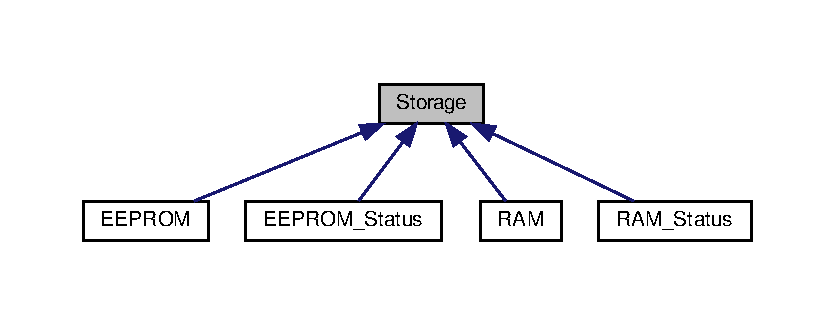
\includegraphics[width=350pt]{class_storage__inherit__graph}
\end{center}
\end{figure}
\subsection*{Öffentliche Methoden}
\begin{DoxyCompactItemize}
\item 
\textbf{ Storage} ()
\item 
void \textbf{ set\+Params} (std\+::string command, int row\+\_\+length, int rows, std\+::string file\+Path)
\item 
virtual \textbf{ $\sim$\+Storage} ()
\item 
void \textbf{ print\+Raw\+Vector} ()
\item 
string \textbf{ get\+Raw\+Data} ()
\item 
void \textbf{ print\+Vector} (std\+::vector$<$ int $>$ const \&v)
\item 
void \textbf{ print\+Byte\+Vector} ()
\item 
void \textbf{ print\+Byte\+Vector\+Short} ()
\item 
void \textbf{ read\+Storage} ()
\item 
void \textbf{ read\+Storage} (int Position)
\item 
void \textbf{ hex\+String2int} (std\+::string src, std\+::vector$<$ int $>$ \&target)
\item 
int \textbf{ char2int} (char input)
\item 
void \textbf{ diff\+Bytes\+With} (\textbf{ Storage} $\ast$last, vector$<$ int $>$ exclude\+Bytes=vector$<$ int $>$(), bool write\+Into\+Json\+File=true, std\+::string comment=\char`\"{}\char`\"{})
\end{DoxyCompactItemize}
\subsection*{Öffentliche Attribute}
\begin{DoxyCompactItemize}
\item 
std\+::vector$<$ string $>$ \textbf{ raw}
\item 
std\+::vector$<$ int $>$ \textbf{ bytes}
\item 
bool \textbf{ work\+\_\+offline}
\end{DoxyCompactItemize}
\subsection*{Geschützte Methoden}
\begin{DoxyCompactItemize}
\item 
void \textbf{ progress\+Bar} (int num, int end, std\+::string txt)
\item 
std\+::string \textbf{ remove\+Special\+Char\+From\+String} (std\+::string \&txt)
\item 
bool \textbf{ get\+Bit} (unsigned char byte, int position)
\end{DoxyCompactItemize}


\subsection{Beschreibung der Konstruktoren und Destruktoren}
\mbox{\label{class_storage_a80ef6af5e4c9fd4424ae16e808d05291}} 
\index{Storage@{Storage}!Storage@{Storage}}
\index{Storage@{Storage}!Storage@{Storage}}
\subsubsection{Storage()}
{\footnotesize\ttfamily Storage\+::\+Storage (\begin{DoxyParamCaption}{ }\end{DoxyParamCaption})}

\mbox{\label{class_storage_a73cf30f0a34250396f9eabee7dc5c93d}} 
\index{Storage@{Storage}!````~Storage@{$\sim$\+Storage}}
\index{````~Storage@{$\sim$\+Storage}!Storage@{Storage}}
\subsubsection{$\sim$\+Storage()}
{\footnotesize\ttfamily Storage\+::$\sim$\+Storage (\begin{DoxyParamCaption}{ }\end{DoxyParamCaption})\hspace{0.3cm}{\ttfamily [virtual]}}



\subsection{Dokumentation der Elementfunktionen}
\mbox{\label{class_storage_af467ed6bef46d8d7f5286ae06d9f3289}} 
\index{Storage@{Storage}!char2int@{char2int}}
\index{char2int@{char2int}!Storage@{Storage}}
\subsubsection{char2int()}
{\footnotesize\ttfamily int Storage\+::char2int (\begin{DoxyParamCaption}\item[{char}]{input }\end{DoxyParamCaption})}

\mbox{\label{class_storage_af785114f92fc0ace0eedf9847db00c44}} 
\index{Storage@{Storage}!diff\+Bytes\+With@{diff\+Bytes\+With}}
\index{diff\+Bytes\+With@{diff\+Bytes\+With}!Storage@{Storage}}
\subsubsection{diff\+Bytes\+With()}
{\footnotesize\ttfamily void Storage\+::diff\+Bytes\+With (\begin{DoxyParamCaption}\item[{\textbf{ Storage} $\ast$}]{last,  }\item[{vector$<$ int $>$}]{exclude\+Bytes = {\ttfamily vector$<$int$>$()},  }\item[{bool}]{write\+Into\+Json\+File = {\ttfamily true},  }\item[{std\+::string}]{comment = {\ttfamily \char`\"{}\char`\"{}} }\end{DoxyParamCaption})}

Hier ist ein Graph, der zeigt, was diese Funktion aufruft\+:\nopagebreak
\begin{figure}[H]
\begin{center}
\leavevmode
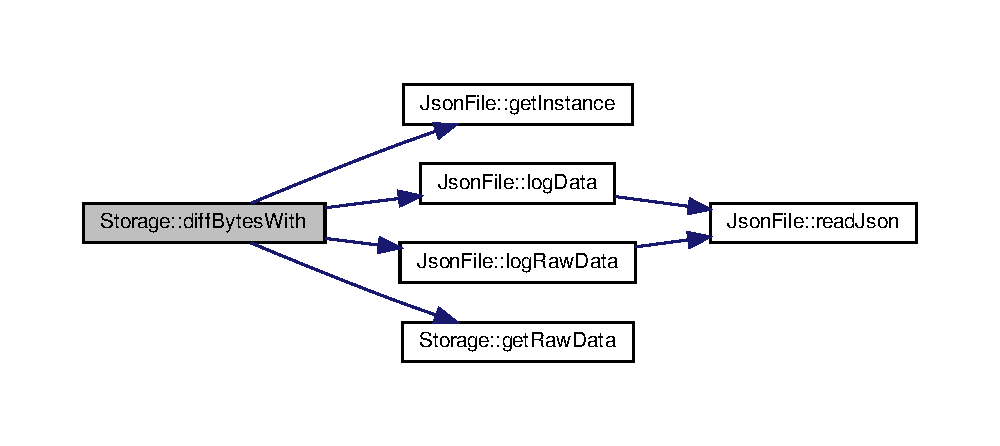
\includegraphics[width=350pt]{class_storage_af785114f92fc0ace0eedf9847db00c44_cgraph}
\end{center}
\end{figure}
\mbox{\label{class_storage_aaaaec44a9862aef40bba754f49c2ee41}} 
\index{Storage@{Storage}!get\+Bit@{get\+Bit}}
\index{get\+Bit@{get\+Bit}!Storage@{Storage}}
\subsubsection{get\+Bit()}
{\footnotesize\ttfamily bool Storage\+::get\+Bit (\begin{DoxyParamCaption}\item[{unsigned char}]{byte,  }\item[{int}]{position }\end{DoxyParamCaption})\hspace{0.3cm}{\ttfamily [protected]}}

\mbox{\label{class_storage_af3ccaf7489cfef2e9cb610989dcd4817}} 
\index{Storage@{Storage}!get\+Raw\+Data@{get\+Raw\+Data}}
\index{get\+Raw\+Data@{get\+Raw\+Data}!Storage@{Storage}}
\subsubsection{get\+Raw\+Data()}
{\footnotesize\ttfamily string Storage\+::get\+Raw\+Data (\begin{DoxyParamCaption}{ }\end{DoxyParamCaption})}

\mbox{\label{class_storage_ae18375a7a591503e52e385db8e0233a5}} 
\index{Storage@{Storage}!hex\+String2int@{hex\+String2int}}
\index{hex\+String2int@{hex\+String2int}!Storage@{Storage}}
\subsubsection{hex\+String2int()}
{\footnotesize\ttfamily void Storage\+::hex\+String2int (\begin{DoxyParamCaption}\item[{std\+::string}]{src,  }\item[{std\+::vector$<$ int $>$ \&}]{target }\end{DoxyParamCaption})}

\mbox{\label{class_storage_a9e306e4e378e00197d5d024b0421805b}} 
\index{Storage@{Storage}!print\+Byte\+Vector@{print\+Byte\+Vector}}
\index{print\+Byte\+Vector@{print\+Byte\+Vector}!Storage@{Storage}}
\subsubsection{print\+Byte\+Vector()}
{\footnotesize\ttfamily void Storage\+::print\+Byte\+Vector (\begin{DoxyParamCaption}{ }\end{DoxyParamCaption})}

\mbox{\label{class_storage_af2c170f7521a99468e334c95a542f399}} 
\index{Storage@{Storage}!print\+Byte\+Vector\+Short@{print\+Byte\+Vector\+Short}}
\index{print\+Byte\+Vector\+Short@{print\+Byte\+Vector\+Short}!Storage@{Storage}}
\subsubsection{print\+Byte\+Vector\+Short()}
{\footnotesize\ttfamily void Storage\+::print\+Byte\+Vector\+Short (\begin{DoxyParamCaption}{ }\end{DoxyParamCaption})}

\mbox{\label{class_storage_a9c875a4c268b989f13aabf299ff6268e}} 
\index{Storage@{Storage}!print\+Raw\+Vector@{print\+Raw\+Vector}}
\index{print\+Raw\+Vector@{print\+Raw\+Vector}!Storage@{Storage}}
\subsubsection{print\+Raw\+Vector()}
{\footnotesize\ttfamily void Storage\+::print\+Raw\+Vector (\begin{DoxyParamCaption}{ }\end{DoxyParamCaption})}

\mbox{\label{class_storage_ad053d05f06bfa7eb034457902bfcf840}} 
\index{Storage@{Storage}!print\+Vector@{print\+Vector}}
\index{print\+Vector@{print\+Vector}!Storage@{Storage}}
\subsubsection{print\+Vector()}
{\footnotesize\ttfamily void Storage\+::print\+Vector (\begin{DoxyParamCaption}\item[{std\+::vector$<$ int $>$ const \&}]{v }\end{DoxyParamCaption})}

\mbox{\label{class_storage_a9952af852b2676ede3fa5b3cd0b1be63}} 
\index{Storage@{Storage}!progress\+Bar@{progress\+Bar}}
\index{progress\+Bar@{progress\+Bar}!Storage@{Storage}}
\subsubsection{progress\+Bar()}
{\footnotesize\ttfamily void Storage\+::progress\+Bar (\begin{DoxyParamCaption}\item[{int}]{num,  }\item[{int}]{end,  }\item[{std\+::string}]{txt }\end{DoxyParamCaption})\hspace{0.3cm}{\ttfamily [protected]}}

\mbox{\label{class_storage_aff274782e2d75969248c380c1869bd0c}} 
\index{Storage@{Storage}!read\+Storage@{read\+Storage}}
\index{read\+Storage@{read\+Storage}!Storage@{Storage}}
\subsubsection{read\+Storage()\hspace{0.1cm}{\footnotesize\ttfamily [1/2]}}
{\footnotesize\ttfamily void Storage\+::read\+Storage (\begin{DoxyParamCaption}{ }\end{DoxyParamCaption})}

\mbox{\label{class_storage_a6b8c995a4ee57633e7c612bdb1714fbb}} 
\index{Storage@{Storage}!read\+Storage@{read\+Storage}}
\index{read\+Storage@{read\+Storage}!Storage@{Storage}}
\subsubsection{read\+Storage()\hspace{0.1cm}{\footnotesize\ttfamily [2/2]}}
{\footnotesize\ttfamily void Storage\+::read\+Storage (\begin{DoxyParamCaption}\item[{int}]{Position }\end{DoxyParamCaption})}

Hier ist ein Graph, der zeigt, was diese Funktion aufruft\+:\nopagebreak
\begin{figure}[H]
\begin{center}
\leavevmode
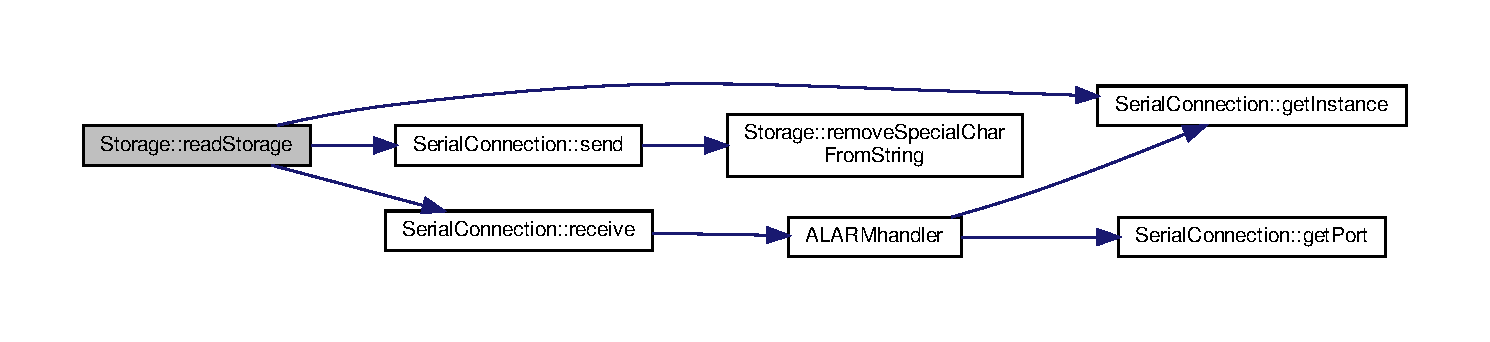
\includegraphics[width=350pt]{class_storage_a6b8c995a4ee57633e7c612bdb1714fbb_cgraph}
\end{center}
\end{figure}
\mbox{\label{class_storage_ad0b9a18790e8a1c56b349c1997ba4315}} 
\index{Storage@{Storage}!remove\+Special\+Char\+From\+String@{remove\+Special\+Char\+From\+String}}
\index{remove\+Special\+Char\+From\+String@{remove\+Special\+Char\+From\+String}!Storage@{Storage}}
\subsubsection{remove\+Special\+Char\+From\+String()}
{\footnotesize\ttfamily string Storage\+::remove\+Special\+Char\+From\+String (\begin{DoxyParamCaption}\item[{std\+::string \&}]{txt }\end{DoxyParamCaption})\hspace{0.3cm}{\ttfamily [protected]}}

\mbox{\label{class_storage_a061f74b18be706398d7d8070d234ad90}} 
\index{Storage@{Storage}!set\+Params@{set\+Params}}
\index{set\+Params@{set\+Params}!Storage@{Storage}}
\subsubsection{set\+Params()}
{\footnotesize\ttfamily void Storage\+::set\+Params (\begin{DoxyParamCaption}\item[{std\+::string}]{command,  }\item[{int}]{row\+\_\+length,  }\item[{int}]{rows,  }\item[{std\+::string}]{file\+Path }\end{DoxyParamCaption})}



\subsection{Dokumentation der Datenelemente}
\mbox{\label{class_storage_a5682d2e69bffe775bcda83a54759de0d}} 
\index{Storage@{Storage}!bytes@{bytes}}
\index{bytes@{bytes}!Storage@{Storage}}
\subsubsection{bytes}
{\footnotesize\ttfamily std\+::vector$<$int$>$ Storage\+::bytes}

\mbox{\label{class_storage_a5c26b6c4b245e3deb8ef3a0da04e6f7b}} 
\index{Storage@{Storage}!raw@{raw}}
\index{raw@{raw}!Storage@{Storage}}
\subsubsection{raw}
{\footnotesize\ttfamily std\+::vector$<$string$>$ Storage\+::raw}

\mbox{\label{class_storage_a76e6060150c2226088365af77fe90385}} 
\index{Storage@{Storage}!work\+\_\+offline@{work\+\_\+offline}}
\index{work\+\_\+offline@{work\+\_\+offline}!Storage@{Storage}}
\subsubsection{work\+\_\+offline}
{\footnotesize\ttfamily bool Storage\+::work\+\_\+offline}



Die Dokumentation für diese Klasse wurde erzeugt aufgrund der Dateien\+:\begin{DoxyCompactItemize}
\item 
/home/cjg8251/\+Desktop/\+Jura\+Coffee\+Memory/\textbf{ Storage.\+hpp}\item 
/home/cjg8251/\+Desktop/\+Jura\+Coffee\+Memory/\textbf{ Storage.\+cpp}\end{DoxyCompactItemize}

\chapter{Datei-\/\+Dokumentation}
\section{/home/cjg8251/\+Desktop/\+Jura\+Coffee\+Memory/color-\/definitions.h-\/\+Dateireferenz}
\label{color-definitions_8h}\index{/home/cjg8251/\+Desktop/\+Jura\+Coffee\+Memory/color-\/definitions.\+h@{/home/cjg8251/\+Desktop/\+Jura\+Coffee\+Memory/color-\/definitions.\+h}}
Dieser Graph zeigt, welche Datei direkt oder indirekt diese Datei enthält\+:\nopagebreak
\begin{figure}[H]
\begin{center}
\leavevmode
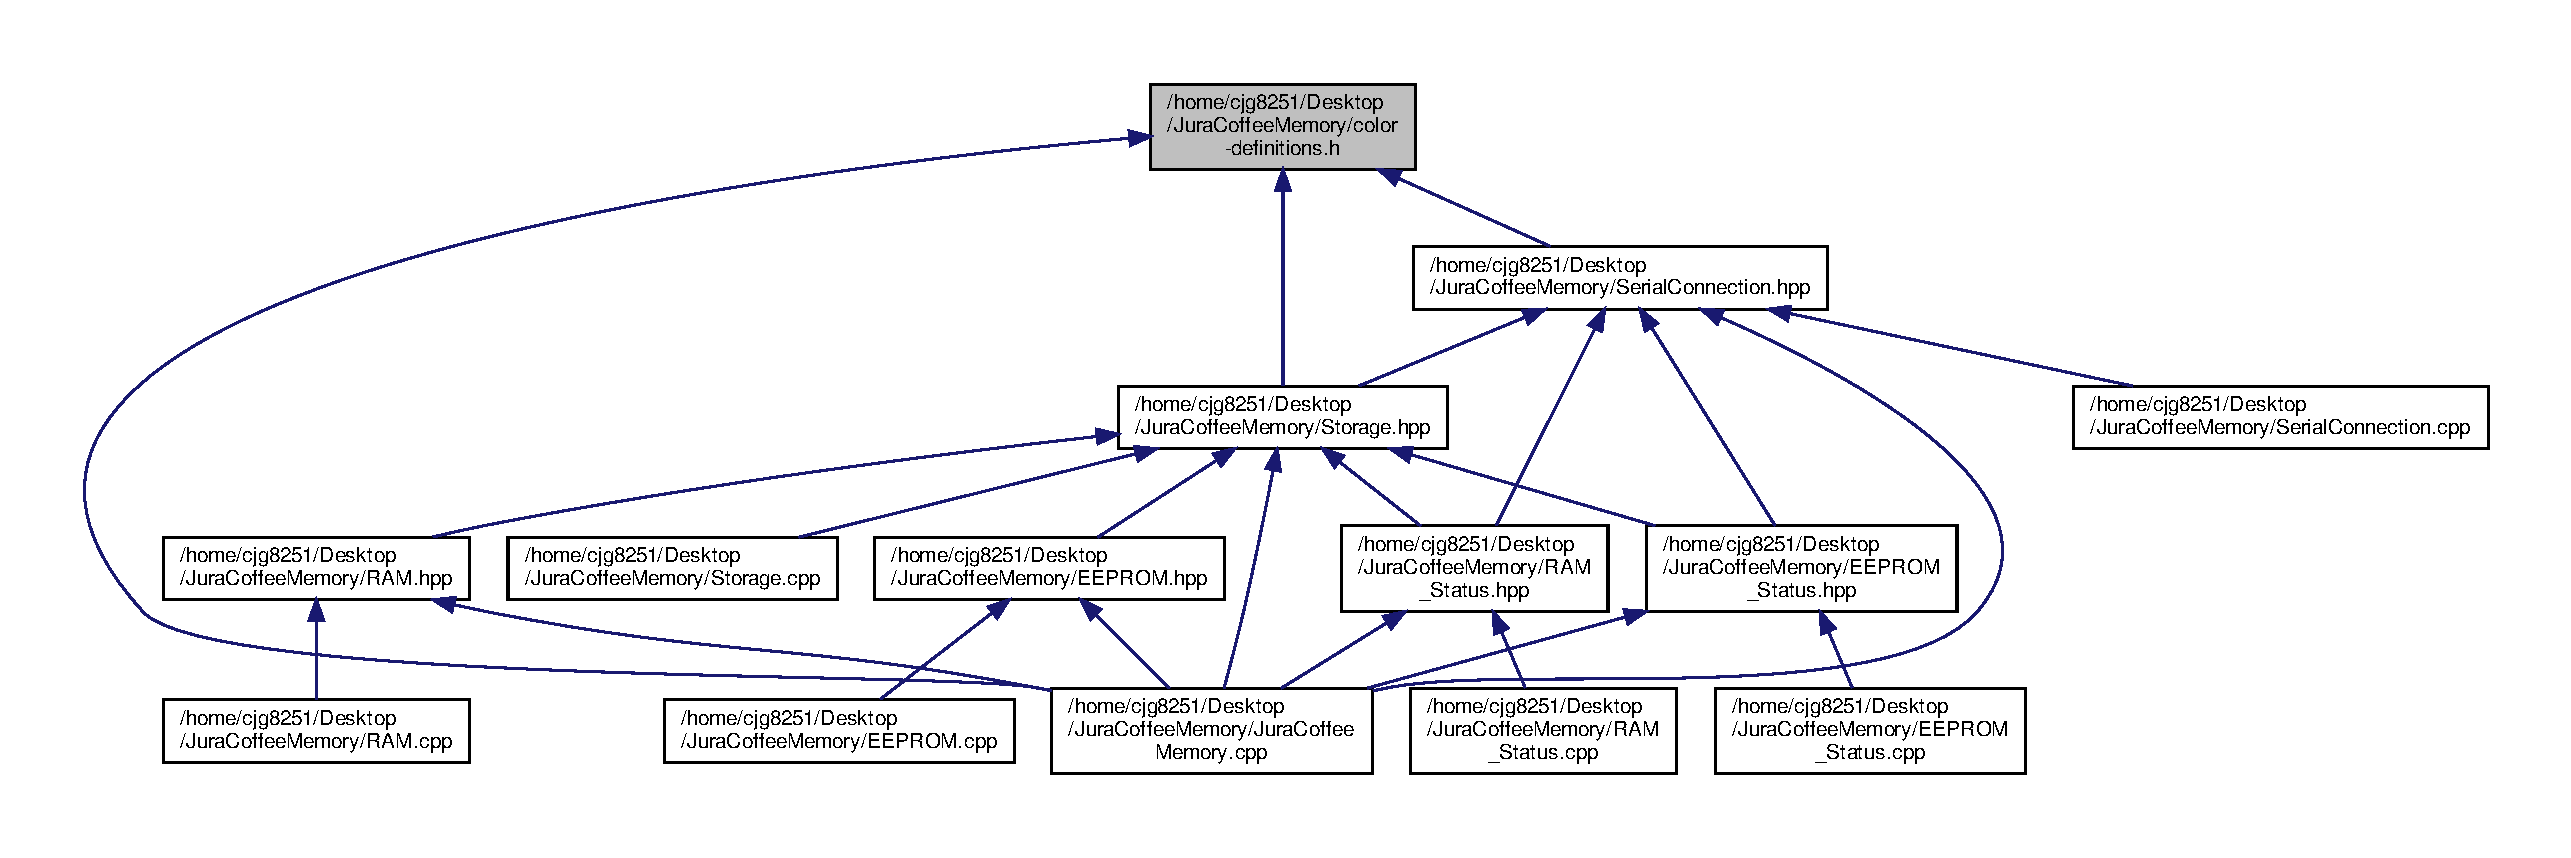
\includegraphics[width=350pt]{color-definitions_8h__dep__incl}
\end{center}
\end{figure}
\subsection*{Makrodefinitionen}
\begin{DoxyCompactItemize}
\item 
\#define \textbf{ C\+O\+L\+O\+R\+\_\+reset}~\char`\"{}\textbackslash{}033[0m\char`\"{}
\item 
\#define \textbf{ C\+O\+L\+O\+R\+\_\+bold}~\char`\"{}\textbackslash{}033[1m\char`\"{}
\item 
\#define \textbf{ C\+O\+L\+O\+R\+\_\+underline}~\char`\"{}\textbackslash{}033[4m\char`\"{}
\item 
\#define \textbf{ C\+O\+L\+O\+R\+\_\+swap\+\_\+\+F\+G\+\_\+\+BG}~\char`\"{}\textbackslash{}033[7m\char`\"{}
\item 
\#define \textbf{ C\+O\+L\+O\+R\+\_\+\+F\+G\+\_\+black}~\char`\"{}\textbackslash{}033[30m\char`\"{}
\item 
\#define \textbf{ C\+O\+L\+O\+R\+\_\+\+F\+G\+\_\+red}~\char`\"{}\textbackslash{}033[31m\char`\"{}
\item 
\#define \textbf{ C\+O\+L\+O\+R\+\_\+\+F\+G\+\_\+green}~\char`\"{}\textbackslash{}033[32m\char`\"{}
\item 
\#define \textbf{ C\+O\+L\+O\+R\+\_\+\+F\+G\+\_\+yellow}~\char`\"{}\textbackslash{}033[33m\char`\"{}
\item 
\#define \textbf{ C\+O\+L\+O\+R\+\_\+\+F\+G\+\_\+blue}~\char`\"{}\textbackslash{}033[94m\char`\"{}
\item 
\#define \textbf{ C\+O\+L\+O\+R\+\_\+\+F\+G\+\_\+magenta}~\char`\"{}\textbackslash{}033[35m\char`\"{}
\item 
\#define \textbf{ C\+O\+L\+O\+R\+\_\+\+F\+G\+\_\+cyan}~\char`\"{}\textbackslash{}033[36m\char`\"{}
\item 
\#define \textbf{ C\+O\+L\+O\+R\+\_\+\+F\+G\+\_\+white}~\char`\"{}\textbackslash{}033[37m\char`\"{}
\item 
\#define \textbf{ C\+O\+L\+O\+R\+\_\+\+B\+G\+\_\+black}~\char`\"{}\textbackslash{}033[40m\char`\"{}
\item 
\#define \textbf{ C\+O\+L\+O\+R\+\_\+\+B\+G\+\_\+red}~\char`\"{}\textbackslash{}033[41m\char`\"{}
\item 
\#define \textbf{ C\+O\+L\+O\+R\+\_\+\+B\+G\+\_\+green}~\char`\"{}\textbackslash{}033[42m\char`\"{}
\item 
\#define \textbf{ C\+O\+L\+O\+R\+\_\+\+B\+G\+\_\+yellow}~\char`\"{}\textbackslash{}033[43m\char`\"{}
\item 
\#define \textbf{ C\+O\+L\+O\+R\+\_\+\+B\+G\+\_\+blue}~\char`\"{}\textbackslash{}033[44m\char`\"{}
\item 
\#define \textbf{ C\+O\+L\+O\+R\+\_\+\+B\+G\+\_\+magenta}~\char`\"{}\textbackslash{}033[45m\char`\"{}
\item 
\#define \textbf{ C\+O\+L\+O\+R\+\_\+\+B\+G\+\_\+cyan}~\char`\"{}\textbackslash{}033[46m\char`\"{}
\item 
\#define \textbf{ C\+O\+L\+O\+R\+\_\+\+B\+G\+\_\+white}~\char`\"{}\textbackslash{}033[47m\char`\"{}
\end{DoxyCompactItemize}


\subsection{Makro-\/\+Dokumentation}
\mbox{\label{color-definitions_8h_aab82dd2d4f58e18826aec1a6656f546e}} 
\index{color-\/definitions.\+h@{color-\/definitions.\+h}!C\+O\+L\+O\+R\+\_\+\+B\+G\+\_\+black@{C\+O\+L\+O\+R\+\_\+\+B\+G\+\_\+black}}
\index{C\+O\+L\+O\+R\+\_\+\+B\+G\+\_\+black@{C\+O\+L\+O\+R\+\_\+\+B\+G\+\_\+black}!color-\/definitions.\+h@{color-\/definitions.\+h}}
\subsubsection{C\+O\+L\+O\+R\+\_\+\+B\+G\+\_\+black}
{\footnotesize\ttfamily \#define C\+O\+L\+O\+R\+\_\+\+B\+G\+\_\+black~\char`\"{}\textbackslash{}033[40m\char`\"{}}

\mbox{\label{color-definitions_8h_a1482ba0e92e85f2f9fe76b5121314134}} 
\index{color-\/definitions.\+h@{color-\/definitions.\+h}!C\+O\+L\+O\+R\+\_\+\+B\+G\+\_\+blue@{C\+O\+L\+O\+R\+\_\+\+B\+G\+\_\+blue}}
\index{C\+O\+L\+O\+R\+\_\+\+B\+G\+\_\+blue@{C\+O\+L\+O\+R\+\_\+\+B\+G\+\_\+blue}!color-\/definitions.\+h@{color-\/definitions.\+h}}
\subsubsection{C\+O\+L\+O\+R\+\_\+\+B\+G\+\_\+blue}
{\footnotesize\ttfamily \#define C\+O\+L\+O\+R\+\_\+\+B\+G\+\_\+blue~\char`\"{}\textbackslash{}033[44m\char`\"{}}

\mbox{\label{color-definitions_8h_af794611fa0e728beb3fb63e2edd00033}} 
\index{color-\/definitions.\+h@{color-\/definitions.\+h}!C\+O\+L\+O\+R\+\_\+\+B\+G\+\_\+cyan@{C\+O\+L\+O\+R\+\_\+\+B\+G\+\_\+cyan}}
\index{C\+O\+L\+O\+R\+\_\+\+B\+G\+\_\+cyan@{C\+O\+L\+O\+R\+\_\+\+B\+G\+\_\+cyan}!color-\/definitions.\+h@{color-\/definitions.\+h}}
\subsubsection{C\+O\+L\+O\+R\+\_\+\+B\+G\+\_\+cyan}
{\footnotesize\ttfamily \#define C\+O\+L\+O\+R\+\_\+\+B\+G\+\_\+cyan~\char`\"{}\textbackslash{}033[46m\char`\"{}}

\mbox{\label{color-definitions_8h_a1d37aa63539d3e75eaa6e5d4557775b2}} 
\index{color-\/definitions.\+h@{color-\/definitions.\+h}!C\+O\+L\+O\+R\+\_\+\+B\+G\+\_\+green@{C\+O\+L\+O\+R\+\_\+\+B\+G\+\_\+green}}
\index{C\+O\+L\+O\+R\+\_\+\+B\+G\+\_\+green@{C\+O\+L\+O\+R\+\_\+\+B\+G\+\_\+green}!color-\/definitions.\+h@{color-\/definitions.\+h}}
\subsubsection{C\+O\+L\+O\+R\+\_\+\+B\+G\+\_\+green}
{\footnotesize\ttfamily \#define C\+O\+L\+O\+R\+\_\+\+B\+G\+\_\+green~\char`\"{}\textbackslash{}033[42m\char`\"{}}

\mbox{\label{color-definitions_8h_a4f5e2765872d6b69165ac5f7de286255}} 
\index{color-\/definitions.\+h@{color-\/definitions.\+h}!C\+O\+L\+O\+R\+\_\+\+B\+G\+\_\+magenta@{C\+O\+L\+O\+R\+\_\+\+B\+G\+\_\+magenta}}
\index{C\+O\+L\+O\+R\+\_\+\+B\+G\+\_\+magenta@{C\+O\+L\+O\+R\+\_\+\+B\+G\+\_\+magenta}!color-\/definitions.\+h@{color-\/definitions.\+h}}
\subsubsection{C\+O\+L\+O\+R\+\_\+\+B\+G\+\_\+magenta}
{\footnotesize\ttfamily \#define C\+O\+L\+O\+R\+\_\+\+B\+G\+\_\+magenta~\char`\"{}\textbackslash{}033[45m\char`\"{}}

\mbox{\label{color-definitions_8h_a5db5d6f0efdbc8cf1664f07cbf58d300}} 
\index{color-\/definitions.\+h@{color-\/definitions.\+h}!C\+O\+L\+O\+R\+\_\+\+B\+G\+\_\+red@{C\+O\+L\+O\+R\+\_\+\+B\+G\+\_\+red}}
\index{C\+O\+L\+O\+R\+\_\+\+B\+G\+\_\+red@{C\+O\+L\+O\+R\+\_\+\+B\+G\+\_\+red}!color-\/definitions.\+h@{color-\/definitions.\+h}}
\subsubsection{C\+O\+L\+O\+R\+\_\+\+B\+G\+\_\+red}
{\footnotesize\ttfamily \#define C\+O\+L\+O\+R\+\_\+\+B\+G\+\_\+red~\char`\"{}\textbackslash{}033[41m\char`\"{}}

\mbox{\label{color-definitions_8h_ae29251e3dd83cfb9ff673634e5bce3f1}} 
\index{color-\/definitions.\+h@{color-\/definitions.\+h}!C\+O\+L\+O\+R\+\_\+\+B\+G\+\_\+white@{C\+O\+L\+O\+R\+\_\+\+B\+G\+\_\+white}}
\index{C\+O\+L\+O\+R\+\_\+\+B\+G\+\_\+white@{C\+O\+L\+O\+R\+\_\+\+B\+G\+\_\+white}!color-\/definitions.\+h@{color-\/definitions.\+h}}
\subsubsection{C\+O\+L\+O\+R\+\_\+\+B\+G\+\_\+white}
{\footnotesize\ttfamily \#define C\+O\+L\+O\+R\+\_\+\+B\+G\+\_\+white~\char`\"{}\textbackslash{}033[47m\char`\"{}}

\mbox{\label{color-definitions_8h_abf2a94657f31a9dafe2a895e6dc93c22}} 
\index{color-\/definitions.\+h@{color-\/definitions.\+h}!C\+O\+L\+O\+R\+\_\+\+B\+G\+\_\+yellow@{C\+O\+L\+O\+R\+\_\+\+B\+G\+\_\+yellow}}
\index{C\+O\+L\+O\+R\+\_\+\+B\+G\+\_\+yellow@{C\+O\+L\+O\+R\+\_\+\+B\+G\+\_\+yellow}!color-\/definitions.\+h@{color-\/definitions.\+h}}
\subsubsection{C\+O\+L\+O\+R\+\_\+\+B\+G\+\_\+yellow}
{\footnotesize\ttfamily \#define C\+O\+L\+O\+R\+\_\+\+B\+G\+\_\+yellow~\char`\"{}\textbackslash{}033[43m\char`\"{}}

\mbox{\label{color-definitions_8h_a979ec5f91fbc459658feea48a2c8c9d2}} 
\index{color-\/definitions.\+h@{color-\/definitions.\+h}!C\+O\+L\+O\+R\+\_\+bold@{C\+O\+L\+O\+R\+\_\+bold}}
\index{C\+O\+L\+O\+R\+\_\+bold@{C\+O\+L\+O\+R\+\_\+bold}!color-\/definitions.\+h@{color-\/definitions.\+h}}
\subsubsection{C\+O\+L\+O\+R\+\_\+bold}
{\footnotesize\ttfamily \#define C\+O\+L\+O\+R\+\_\+bold~\char`\"{}\textbackslash{}033[1m\char`\"{}}

\mbox{\label{color-definitions_8h_a81c2fe7c2ec2f6a2e787a9ba1509d83d}} 
\index{color-\/definitions.\+h@{color-\/definitions.\+h}!C\+O\+L\+O\+R\+\_\+\+F\+G\+\_\+black@{C\+O\+L\+O\+R\+\_\+\+F\+G\+\_\+black}}
\index{C\+O\+L\+O\+R\+\_\+\+F\+G\+\_\+black@{C\+O\+L\+O\+R\+\_\+\+F\+G\+\_\+black}!color-\/definitions.\+h@{color-\/definitions.\+h}}
\subsubsection{C\+O\+L\+O\+R\+\_\+\+F\+G\+\_\+black}
{\footnotesize\ttfamily \#define C\+O\+L\+O\+R\+\_\+\+F\+G\+\_\+black~\char`\"{}\textbackslash{}033[30m\char`\"{}}

\mbox{\label{color-definitions_8h_a7bc55df6abd26a6d8cd824f34bade891}} 
\index{color-\/definitions.\+h@{color-\/definitions.\+h}!C\+O\+L\+O\+R\+\_\+\+F\+G\+\_\+blue@{C\+O\+L\+O\+R\+\_\+\+F\+G\+\_\+blue}}
\index{C\+O\+L\+O\+R\+\_\+\+F\+G\+\_\+blue@{C\+O\+L\+O\+R\+\_\+\+F\+G\+\_\+blue}!color-\/definitions.\+h@{color-\/definitions.\+h}}
\subsubsection{C\+O\+L\+O\+R\+\_\+\+F\+G\+\_\+blue}
{\footnotesize\ttfamily \#define C\+O\+L\+O\+R\+\_\+\+F\+G\+\_\+blue~\char`\"{}\textbackslash{}033[94m\char`\"{}}

\mbox{\label{color-definitions_8h_a658ab7ab021eb03de8bb8f2f13807c11}} 
\index{color-\/definitions.\+h@{color-\/definitions.\+h}!C\+O\+L\+O\+R\+\_\+\+F\+G\+\_\+cyan@{C\+O\+L\+O\+R\+\_\+\+F\+G\+\_\+cyan}}
\index{C\+O\+L\+O\+R\+\_\+\+F\+G\+\_\+cyan@{C\+O\+L\+O\+R\+\_\+\+F\+G\+\_\+cyan}!color-\/definitions.\+h@{color-\/definitions.\+h}}
\subsubsection{C\+O\+L\+O\+R\+\_\+\+F\+G\+\_\+cyan}
{\footnotesize\ttfamily \#define C\+O\+L\+O\+R\+\_\+\+F\+G\+\_\+cyan~\char`\"{}\textbackslash{}033[36m\char`\"{}}

\mbox{\label{color-definitions_8h_af1a5ccc455efa9ce7b9479bac51d9f5c}} 
\index{color-\/definitions.\+h@{color-\/definitions.\+h}!C\+O\+L\+O\+R\+\_\+\+F\+G\+\_\+green@{C\+O\+L\+O\+R\+\_\+\+F\+G\+\_\+green}}
\index{C\+O\+L\+O\+R\+\_\+\+F\+G\+\_\+green@{C\+O\+L\+O\+R\+\_\+\+F\+G\+\_\+green}!color-\/definitions.\+h@{color-\/definitions.\+h}}
\subsubsection{C\+O\+L\+O\+R\+\_\+\+F\+G\+\_\+green}
{\footnotesize\ttfamily \#define C\+O\+L\+O\+R\+\_\+\+F\+G\+\_\+green~\char`\"{}\textbackslash{}033[32m\char`\"{}}

\mbox{\label{color-definitions_8h_a6b5da26e1f50f7250c34b413422e4df9}} 
\index{color-\/definitions.\+h@{color-\/definitions.\+h}!C\+O\+L\+O\+R\+\_\+\+F\+G\+\_\+magenta@{C\+O\+L\+O\+R\+\_\+\+F\+G\+\_\+magenta}}
\index{C\+O\+L\+O\+R\+\_\+\+F\+G\+\_\+magenta@{C\+O\+L\+O\+R\+\_\+\+F\+G\+\_\+magenta}!color-\/definitions.\+h@{color-\/definitions.\+h}}
\subsubsection{C\+O\+L\+O\+R\+\_\+\+F\+G\+\_\+magenta}
{\footnotesize\ttfamily \#define C\+O\+L\+O\+R\+\_\+\+F\+G\+\_\+magenta~\char`\"{}\textbackslash{}033[35m\char`\"{}}

\mbox{\label{color-definitions_8h_a9effefc2479c5aa2b02718d16a72c0c6}} 
\index{color-\/definitions.\+h@{color-\/definitions.\+h}!C\+O\+L\+O\+R\+\_\+\+F\+G\+\_\+red@{C\+O\+L\+O\+R\+\_\+\+F\+G\+\_\+red}}
\index{C\+O\+L\+O\+R\+\_\+\+F\+G\+\_\+red@{C\+O\+L\+O\+R\+\_\+\+F\+G\+\_\+red}!color-\/definitions.\+h@{color-\/definitions.\+h}}
\subsubsection{C\+O\+L\+O\+R\+\_\+\+F\+G\+\_\+red}
{\footnotesize\ttfamily \#define C\+O\+L\+O\+R\+\_\+\+F\+G\+\_\+red~\char`\"{}\textbackslash{}033[31m\char`\"{}}

\mbox{\label{color-definitions_8h_a690d0c3d418290de781c267928ef9c0f}} 
\index{color-\/definitions.\+h@{color-\/definitions.\+h}!C\+O\+L\+O\+R\+\_\+\+F\+G\+\_\+white@{C\+O\+L\+O\+R\+\_\+\+F\+G\+\_\+white}}
\index{C\+O\+L\+O\+R\+\_\+\+F\+G\+\_\+white@{C\+O\+L\+O\+R\+\_\+\+F\+G\+\_\+white}!color-\/definitions.\+h@{color-\/definitions.\+h}}
\subsubsection{C\+O\+L\+O\+R\+\_\+\+F\+G\+\_\+white}
{\footnotesize\ttfamily \#define C\+O\+L\+O\+R\+\_\+\+F\+G\+\_\+white~\char`\"{}\textbackslash{}033[37m\char`\"{}}

\mbox{\label{color-definitions_8h_a20a5fcd4199263095413d3b301d458bd}} 
\index{color-\/definitions.\+h@{color-\/definitions.\+h}!C\+O\+L\+O\+R\+\_\+\+F\+G\+\_\+yellow@{C\+O\+L\+O\+R\+\_\+\+F\+G\+\_\+yellow}}
\index{C\+O\+L\+O\+R\+\_\+\+F\+G\+\_\+yellow@{C\+O\+L\+O\+R\+\_\+\+F\+G\+\_\+yellow}!color-\/definitions.\+h@{color-\/definitions.\+h}}
\subsubsection{C\+O\+L\+O\+R\+\_\+\+F\+G\+\_\+yellow}
{\footnotesize\ttfamily \#define C\+O\+L\+O\+R\+\_\+\+F\+G\+\_\+yellow~\char`\"{}\textbackslash{}033[33m\char`\"{}}

\mbox{\label{color-definitions_8h_a0b36581e7fd946793bc96d1aa29b93be}} 
\index{color-\/definitions.\+h@{color-\/definitions.\+h}!C\+O\+L\+O\+R\+\_\+reset@{C\+O\+L\+O\+R\+\_\+reset}}
\index{C\+O\+L\+O\+R\+\_\+reset@{C\+O\+L\+O\+R\+\_\+reset}!color-\/definitions.\+h@{color-\/definitions.\+h}}
\subsubsection{C\+O\+L\+O\+R\+\_\+reset}
{\footnotesize\ttfamily \#define C\+O\+L\+O\+R\+\_\+reset~\char`\"{}\textbackslash{}033[0m\char`\"{}}

\mbox{\label{color-definitions_8h_aff91c7085dfddae495e201a316e6d338}} 
\index{color-\/definitions.\+h@{color-\/definitions.\+h}!C\+O\+L\+O\+R\+\_\+swap\+\_\+\+F\+G\+\_\+\+BG@{C\+O\+L\+O\+R\+\_\+swap\+\_\+\+F\+G\+\_\+\+BG}}
\index{C\+O\+L\+O\+R\+\_\+swap\+\_\+\+F\+G\+\_\+\+BG@{C\+O\+L\+O\+R\+\_\+swap\+\_\+\+F\+G\+\_\+\+BG}!color-\/definitions.\+h@{color-\/definitions.\+h}}
\subsubsection{C\+O\+L\+O\+R\+\_\+swap\+\_\+\+F\+G\+\_\+\+BG}
{\footnotesize\ttfamily \#define C\+O\+L\+O\+R\+\_\+swap\+\_\+\+F\+G\+\_\+\+BG~\char`\"{}\textbackslash{}033[7m\char`\"{}}

\mbox{\label{color-definitions_8h_a439cc6c67e13cb95b7d6c0d9fd5169c4}} 
\index{color-\/definitions.\+h@{color-\/definitions.\+h}!C\+O\+L\+O\+R\+\_\+underline@{C\+O\+L\+O\+R\+\_\+underline}}
\index{C\+O\+L\+O\+R\+\_\+underline@{C\+O\+L\+O\+R\+\_\+underline}!color-\/definitions.\+h@{color-\/definitions.\+h}}
\subsubsection{C\+O\+L\+O\+R\+\_\+underline}
{\footnotesize\ttfamily \#define C\+O\+L\+O\+R\+\_\+underline~\char`\"{}\textbackslash{}033[4m\char`\"{}}


\section{/home/cjg8251/\+Desktop/\+Jura\+Coffee\+Memory/\+E\+E\+P\+R\+OM.cpp-\/\+Dateireferenz}
\label{_e_e_p_r_o_m_8cpp}\index{/home/cjg8251/\+Desktop/\+Jura\+Coffee\+Memory/\+E\+E\+P\+R\+O\+M.\+cpp@{/home/cjg8251/\+Desktop/\+Jura\+Coffee\+Memory/\+E\+E\+P\+R\+O\+M.\+cpp}}
{\ttfamily \#include \char`\"{}E\+E\+P\+R\+O\+M.\+hpp\char`\"{}}\newline
Include-\/\+Abhängigkeitsdiagramm für E\+E\+P\+R\+O\+M.\+cpp\+:
\nopagebreak
\begin{figure}[H]
\begin{center}
\leavevmode
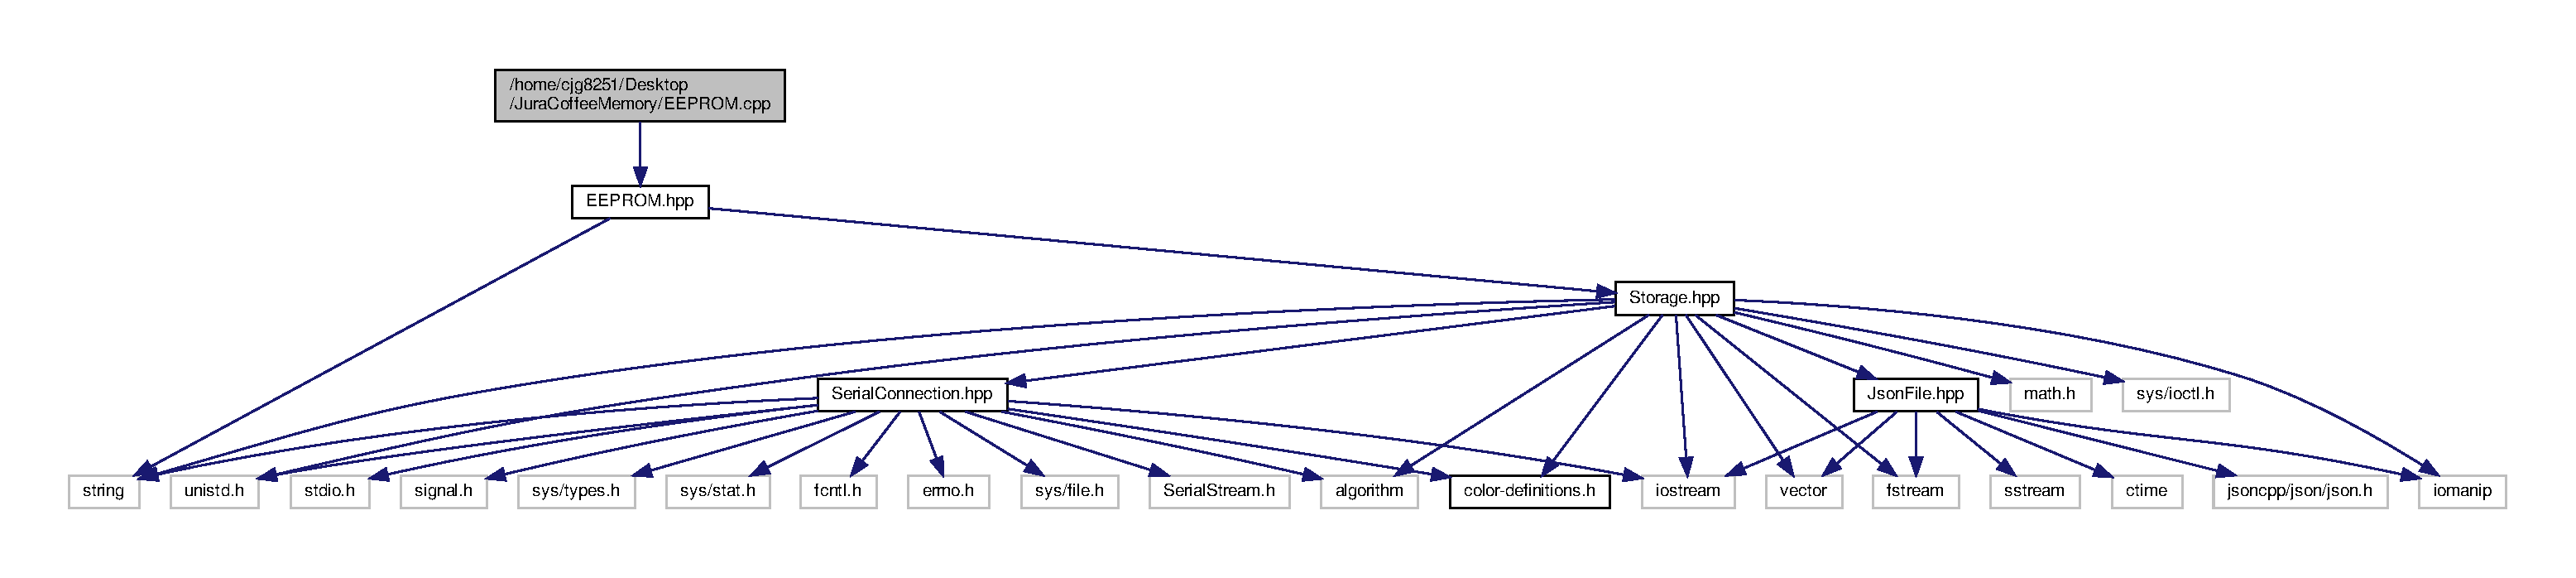
\includegraphics[width=350pt]{_e_e_p_r_o_m_8cpp__incl}
\end{center}
\end{figure}

\section{/home/cjg8251/\+Desktop/\+Jura\+Coffee\+Memory/\+E\+E\+P\+R\+OM.hpp-\/\+Dateireferenz}
\label{_e_e_p_r_o_m_8hpp}\index{/home/cjg8251/\+Desktop/\+Jura\+Coffee\+Memory/\+E\+E\+P\+R\+O\+M.\+hpp@{/home/cjg8251/\+Desktop/\+Jura\+Coffee\+Memory/\+E\+E\+P\+R\+O\+M.\+hpp}}
{\ttfamily \#include $<$string$>$}\newline
{\ttfamily \#include \char`\"{}Storage.\+hpp\char`\"{}}\newline
Include-\/\+Abhängigkeitsdiagramm für E\+E\+P\+R\+O\+M.\+hpp\+:
\nopagebreak
\begin{figure}[H]
\begin{center}
\leavevmode
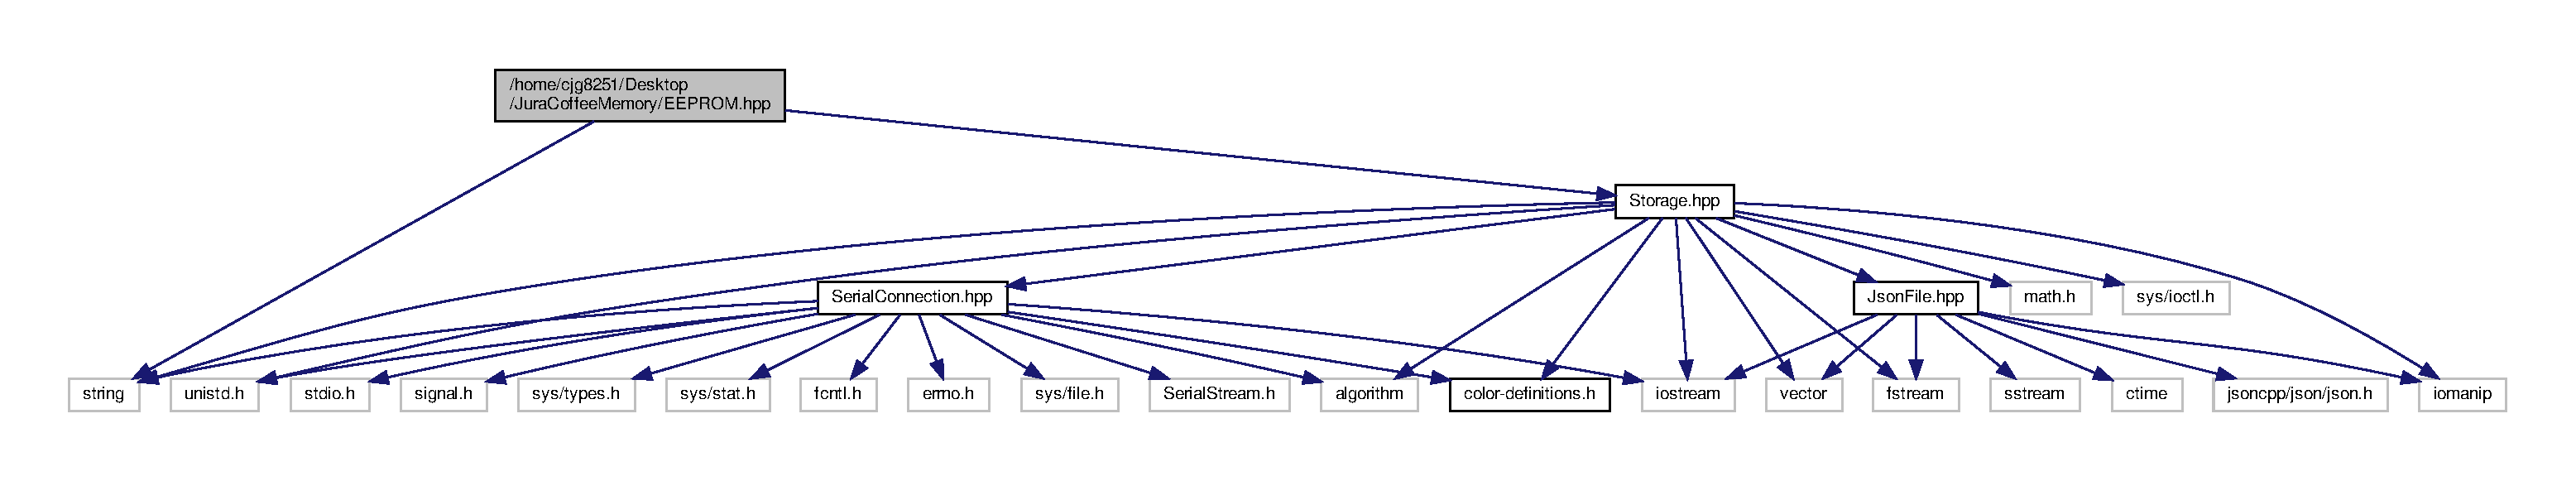
\includegraphics[width=350pt]{_e_e_p_r_o_m_8hpp__incl}
\end{center}
\end{figure}
Dieser Graph zeigt, welche Datei direkt oder indirekt diese Datei enthält\+:
\nopagebreak
\begin{figure}[H]
\begin{center}
\leavevmode
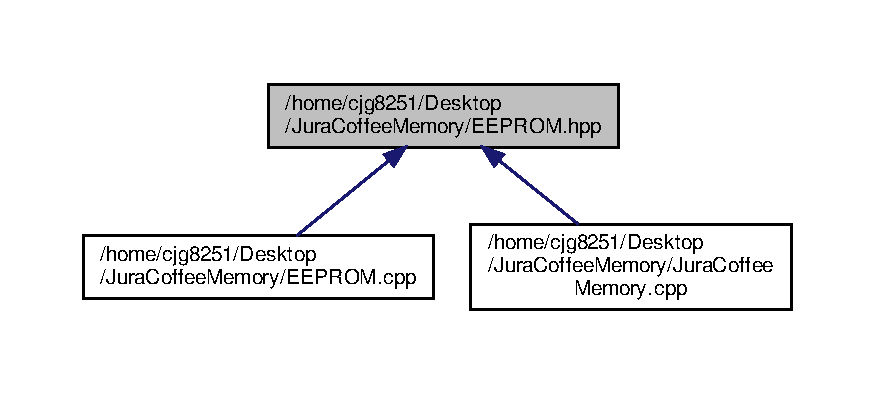
\includegraphics[width=350pt]{_e_e_p_r_o_m_8hpp__dep__incl}
\end{center}
\end{figure}
\subsection*{Klassen}
\begin{DoxyCompactItemize}
\item 
class \textbf{ E\+E\+P\+R\+OM}
\end{DoxyCompactItemize}

\section{/home/cjg8251/\+Desktop/\+Jura\+Coffee\+Memory/\+E\+E\+P\+R\+O\+M\+\_\+\+Status.cpp-\/\+Dateireferenz}
\label{_e_e_p_r_o_m___status_8cpp}\index{/home/cjg8251/\+Desktop/\+Jura\+Coffee\+Memory/\+E\+E\+P\+R\+O\+M\+\_\+\+Status.\+cpp@{/home/cjg8251/\+Desktop/\+Jura\+Coffee\+Memory/\+E\+E\+P\+R\+O\+M\+\_\+\+Status.\+cpp}}
{\ttfamily \#include \char`\"{}E\+E\+P\+R\+O\+M\+\_\+\+Status.\+hpp\char`\"{}}\newline
Include-\/\+Abhängigkeitsdiagramm für E\+E\+P\+R\+O\+M\+\_\+\+Status.\+cpp\+:
\nopagebreak
\begin{figure}[H]
\begin{center}
\leavevmode
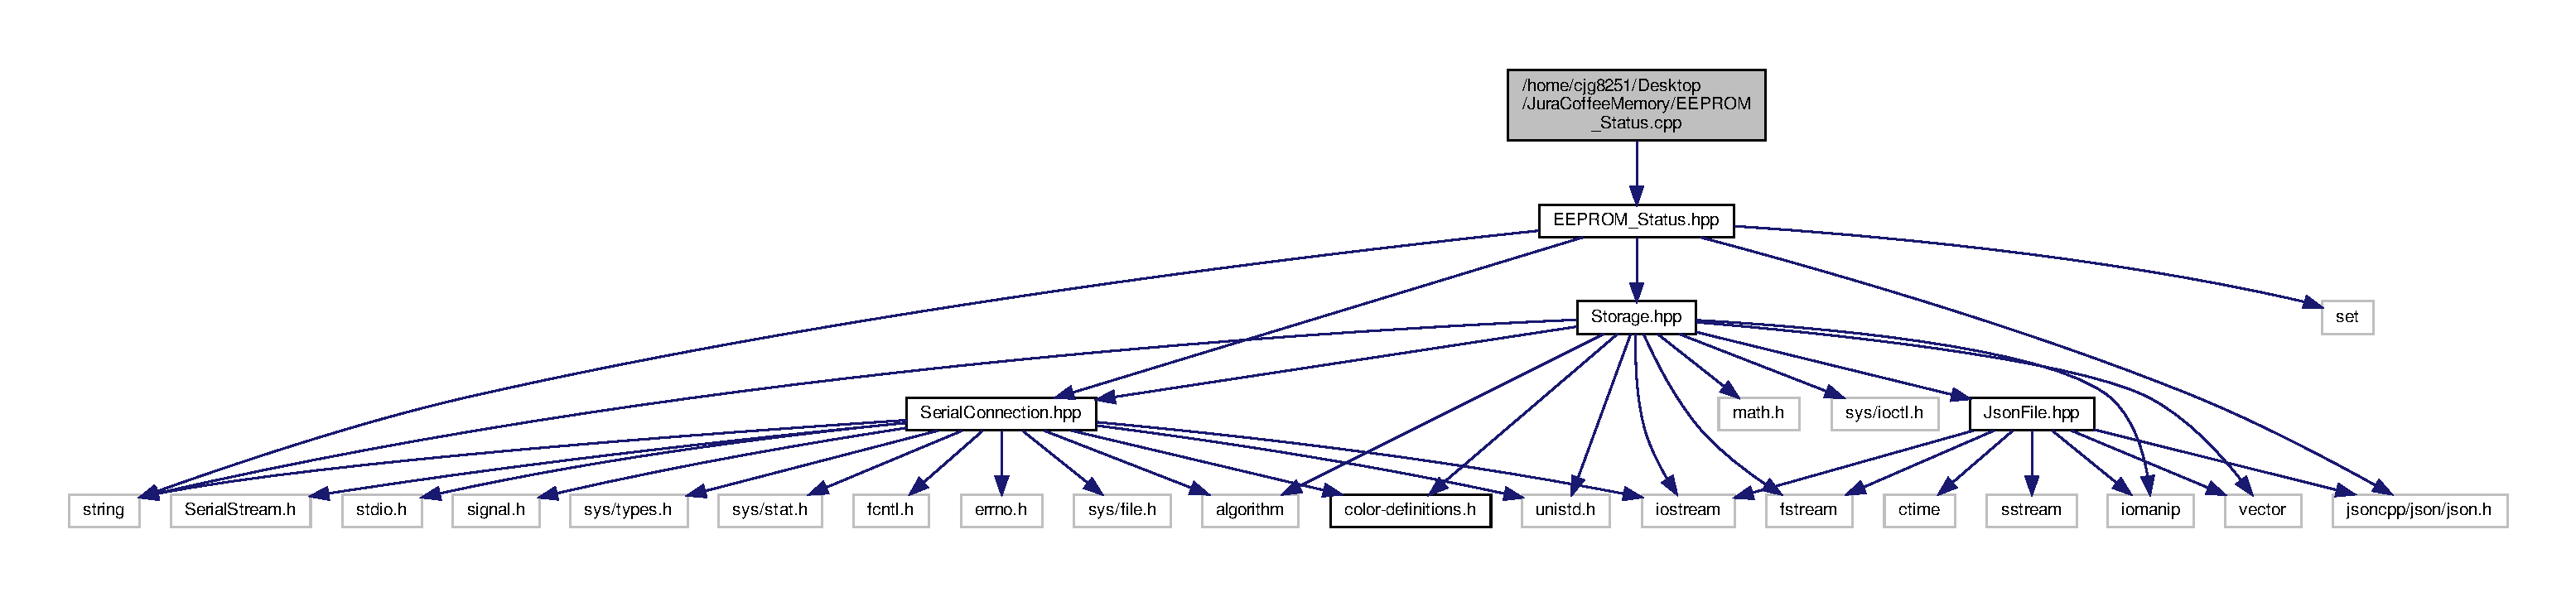
\includegraphics[width=350pt]{_e_e_p_r_o_m___status_8cpp__incl}
\end{center}
\end{figure}

\section{/home/cjg8251/\+Desktop/\+Jura\+Coffee\+Memory/\+E\+E\+P\+R\+O\+M\+\_\+\+Status.hpp-\/\+Dateireferenz}
\label{_e_e_p_r_o_m___status_8hpp}\index{/home/cjg8251/\+Desktop/\+Jura\+Coffee\+Memory/\+E\+E\+P\+R\+O\+M\+\_\+\+Status.\+hpp@{/home/cjg8251/\+Desktop/\+Jura\+Coffee\+Memory/\+E\+E\+P\+R\+O\+M\+\_\+\+Status.\+hpp}}
{\ttfamily \#include $<$string$>$}\newline
{\ttfamily \#include $<$set$>$}\newline
{\ttfamily \#include \char`\"{}Storage.\+hpp\char`\"{}}\newline
{\ttfamily \#include \char`\"{}Serial\+Connection.\+hpp\char`\"{}}\newline
{\ttfamily \#include $<$jsoncpp/json/json.\+h$>$}\newline
Include-\/\+Abhängigkeitsdiagramm für E\+E\+P\+R\+O\+M\+\_\+\+Status.\+hpp\+:
\nopagebreak
\begin{figure}[H]
\begin{center}
\leavevmode
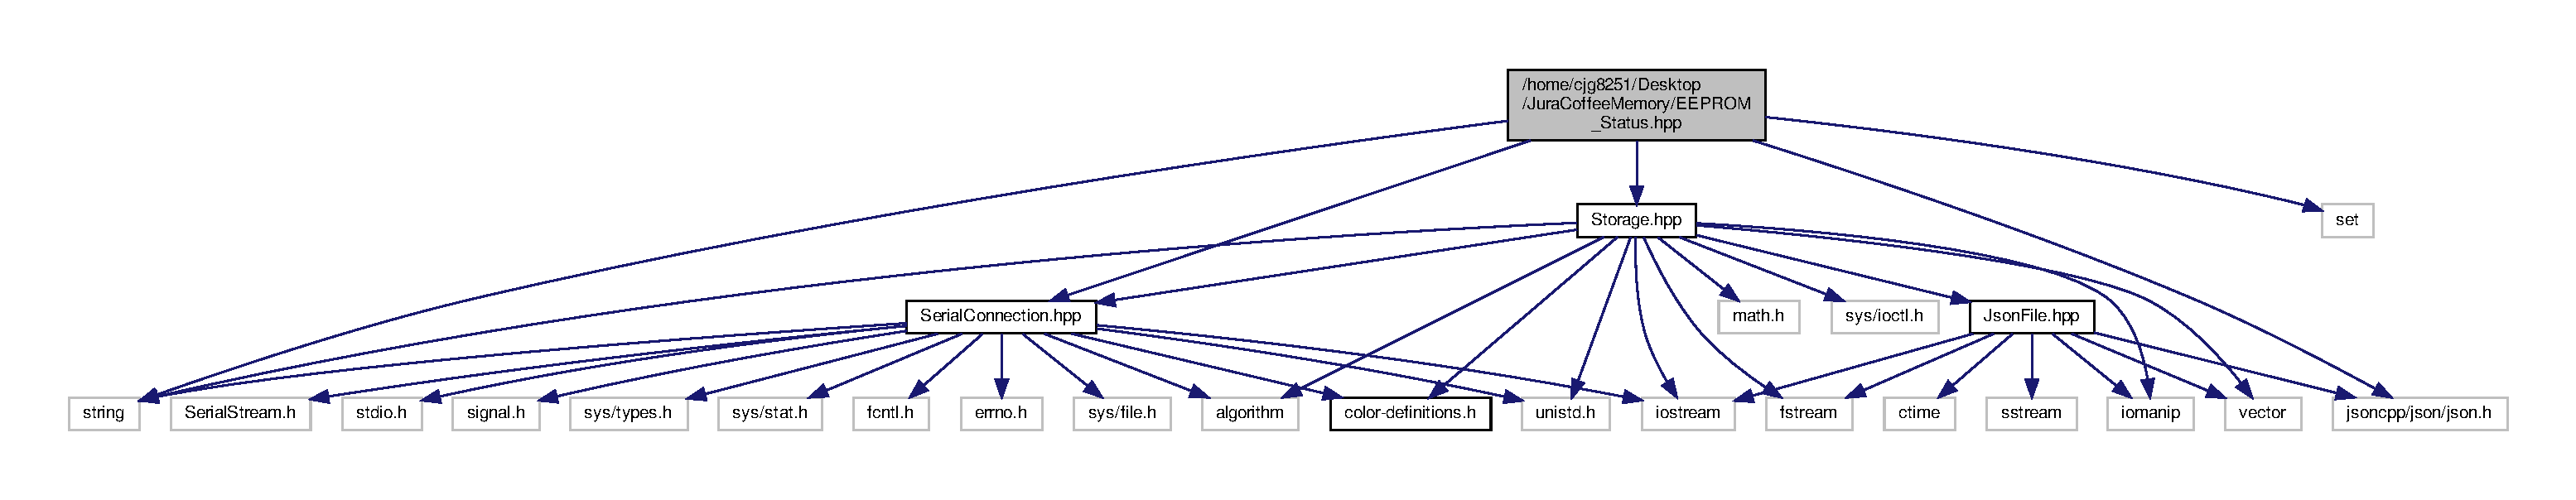
\includegraphics[width=350pt]{_e_e_p_r_o_m___status_8hpp__incl}
\end{center}
\end{figure}
Dieser Graph zeigt, welche Datei direkt oder indirekt diese Datei enthält\+:
\nopagebreak
\begin{figure}[H]
\begin{center}
\leavevmode
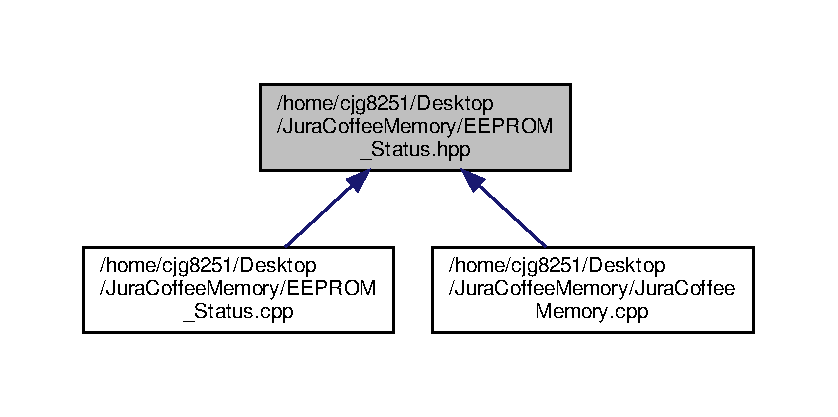
\includegraphics[width=350pt]{_e_e_p_r_o_m___status_8hpp__dep__incl}
\end{center}
\end{figure}
\subsection*{Klassen}
\begin{DoxyCompactItemize}
\item 
struct \textbf{ Entry\+E\+E\+P\+R\+OM}
\item 
class \textbf{ E\+E\+P\+R\+O\+M\+\_\+\+Status}
\end{DoxyCompactItemize}

\section{/home/cjg8251/\+Desktop/\+Jura\+Coffee\+Memory/\+Json\+File.cpp-\/\+Dateireferenz}
\label{_json_file_8cpp}\index{/home/cjg8251/\+Desktop/\+Jura\+Coffee\+Memory/\+Json\+File.\+cpp@{/home/cjg8251/\+Desktop/\+Jura\+Coffee\+Memory/\+Json\+File.\+cpp}}
{\ttfamily \#include \char`\"{}Json\+File.\+hpp\char`\"{}}\newline
Include-\/\+Abhängigkeitsdiagramm für Json\+File.\+cpp\+:\nopagebreak
\begin{figure}[H]
\begin{center}
\leavevmode
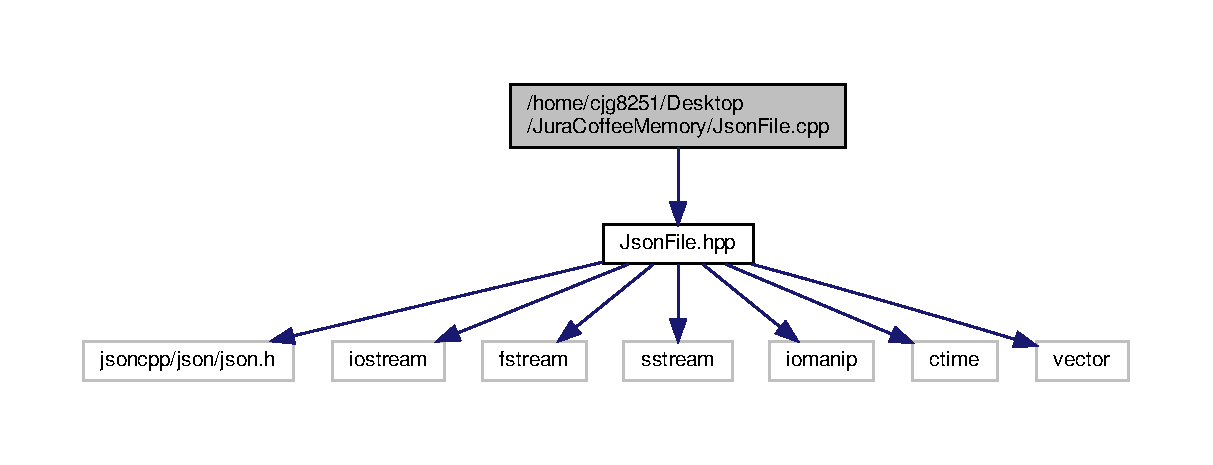
\includegraphics[width=350pt]{_json_file_8cpp__incl}
\end{center}
\end{figure}

\section{/home/cjg8251/\+Desktop/\+Jura\+Coffee\+Memory/\+Json\+File.hpp-\/\+Dateireferenz}
\label{_json_file_8hpp}\index{/home/cjg8251/\+Desktop/\+Jura\+Coffee\+Memory/\+Json\+File.\+hpp@{/home/cjg8251/\+Desktop/\+Jura\+Coffee\+Memory/\+Json\+File.\+hpp}}
{\ttfamily \#include $<$jsoncpp/json/json.\+h$>$}\newline
{\ttfamily \#include $<$iostream$>$}\newline
{\ttfamily \#include $<$fstream$>$}\newline
{\ttfamily \#include $<$sstream$>$}\newline
{\ttfamily \#include $<$iomanip$>$}\newline
{\ttfamily \#include $<$ctime$>$}\newline
{\ttfamily \#include $<$vector$>$}\newline
Include-\/\+Abhängigkeitsdiagramm für Json\+File.\+hpp\+:\nopagebreak
\begin{figure}[H]
\begin{center}
\leavevmode
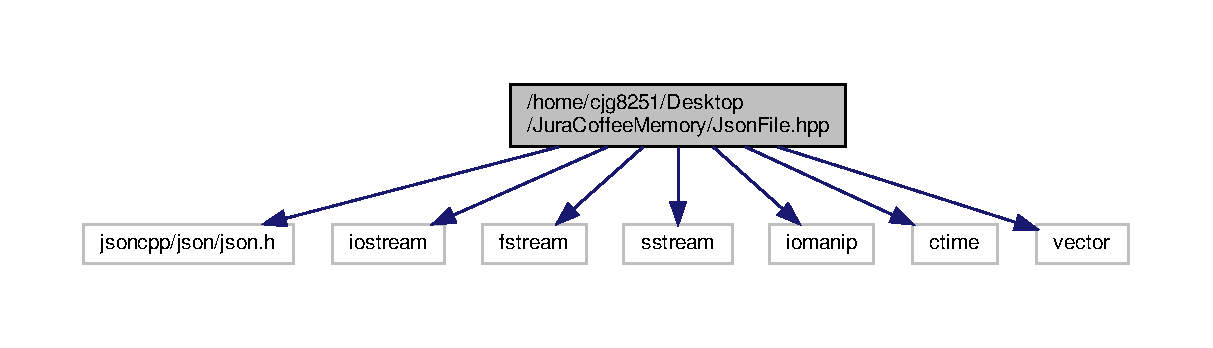
\includegraphics[width=350pt]{_json_file_8hpp__incl}
\end{center}
\end{figure}
Dieser Graph zeigt, welche Datei direkt oder indirekt diese Datei enthält\+:\nopagebreak
\begin{figure}[H]
\begin{center}
\leavevmode
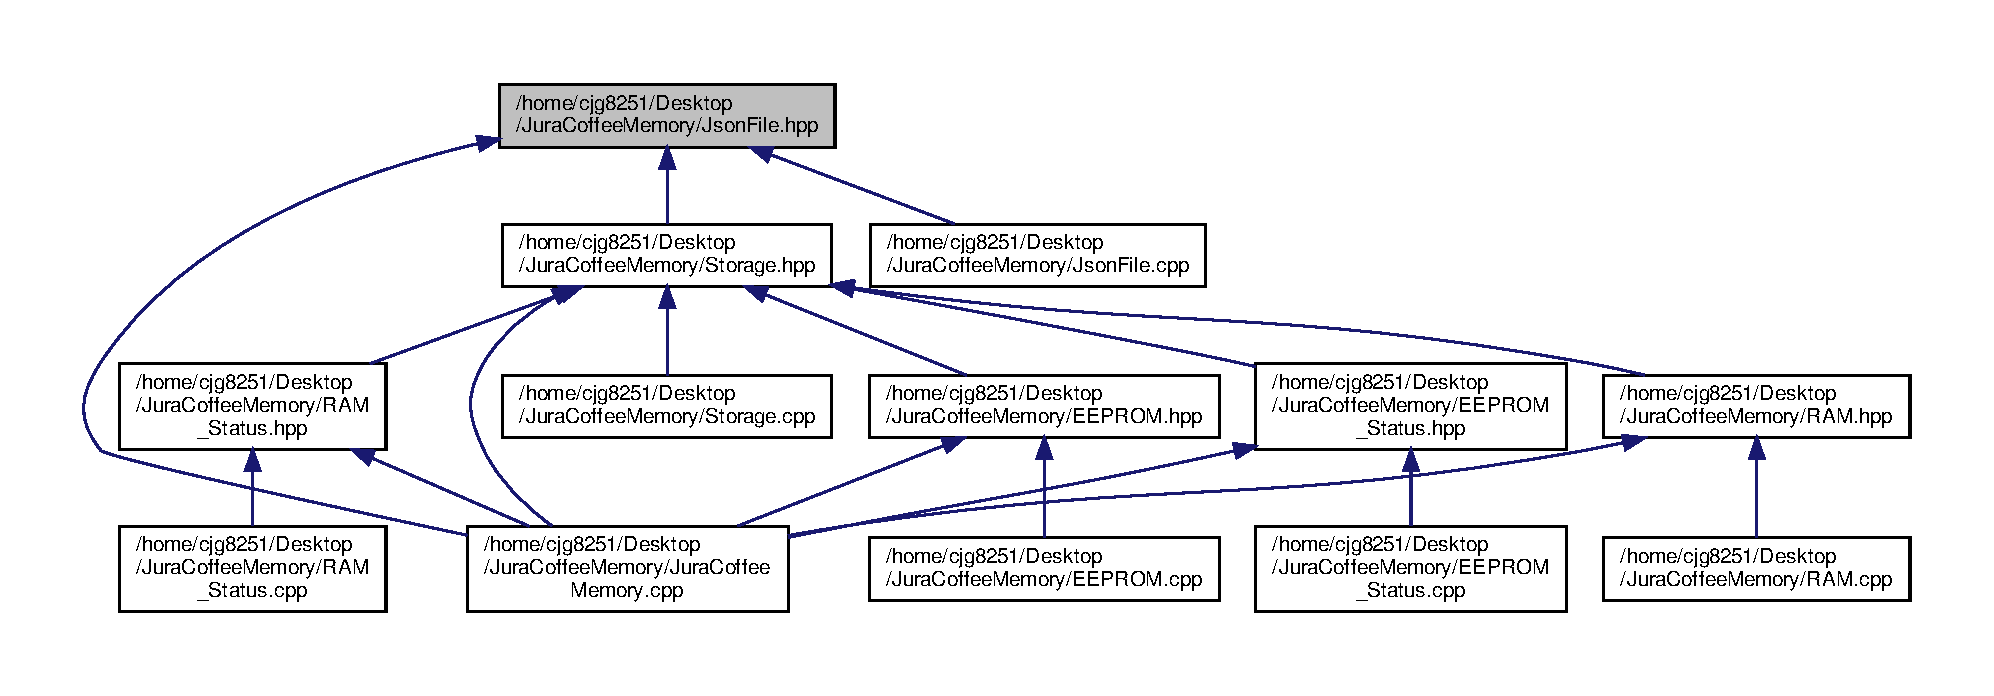
\includegraphics[width=350pt]{_json_file_8hpp__dep__incl}
\end{center}
\end{figure}
\subsection*{Klassen}
\begin{DoxyCompactItemize}
\item 
struct \textbf{ dump}
\item 
struct \textbf{ data}
\item 
class \textbf{ Json\+File}
\end{DoxyCompactItemize}

\section{/home/cjg8251/\+Desktop/\+Jura\+Coffee\+Memory/\+Jura\+Coffee\+Memory.cpp-\/\+Dateireferenz}
\label{_jura_coffee_memory_8cpp}\index{/home/cjg8251/\+Desktop/\+Jura\+Coffee\+Memory/\+Jura\+Coffee\+Memory.\+cpp@{/home/cjg8251/\+Desktop/\+Jura\+Coffee\+Memory/\+Jura\+Coffee\+Memory.\+cpp}}
{\ttfamily \#include $<$iostream$>$}\newline
{\ttfamily \#include $<$cstdlib$>$}\newline
{\ttfamily \#include $<$string$>$}\newline
{\ttfamily \#include $<$vector$>$}\newline
{\ttfamily \#include $<$algorithm$>$}\newline
{\ttfamily \#include $<$unistd.\+h$>$}\newline
{\ttfamily \#include \char`\"{}Storage.\+hpp\char`\"{}}\newline
{\ttfamily \#include \char`\"{}E\+E\+P\+R\+O\+M.\+hpp\char`\"{}}\newline
{\ttfamily \#include \char`\"{}R\+A\+M.\+hpp\char`\"{}}\newline
{\ttfamily \#include \char`\"{}E\+E\+P\+R\+O\+M\+\_\+\+Status.\+hpp\char`\"{}}\newline
{\ttfamily \#include \char`\"{}R\+A\+M\+\_\+\+Status.\+hpp\char`\"{}}\newline
{\ttfamily \#include \char`\"{}Serial\+Connection.\+hpp\char`\"{}}\newline
{\ttfamily \#include \char`\"{}Json\+File.\+hpp\char`\"{}}\newline
{\ttfamily \#include \char`\"{}color-\/definitions.\+h\char`\"{}}\newline
{\ttfamily \#include $<$experimental/filesystem$>$}\newline
{\ttfamily \#include $<$sstream$>$}\newline
Include-\/\+Abhängigkeitsdiagramm für Jura\+Coffee\+Memory.\+cpp\+:
\nopagebreak
\begin{figure}[H]
\begin{center}
\leavevmode
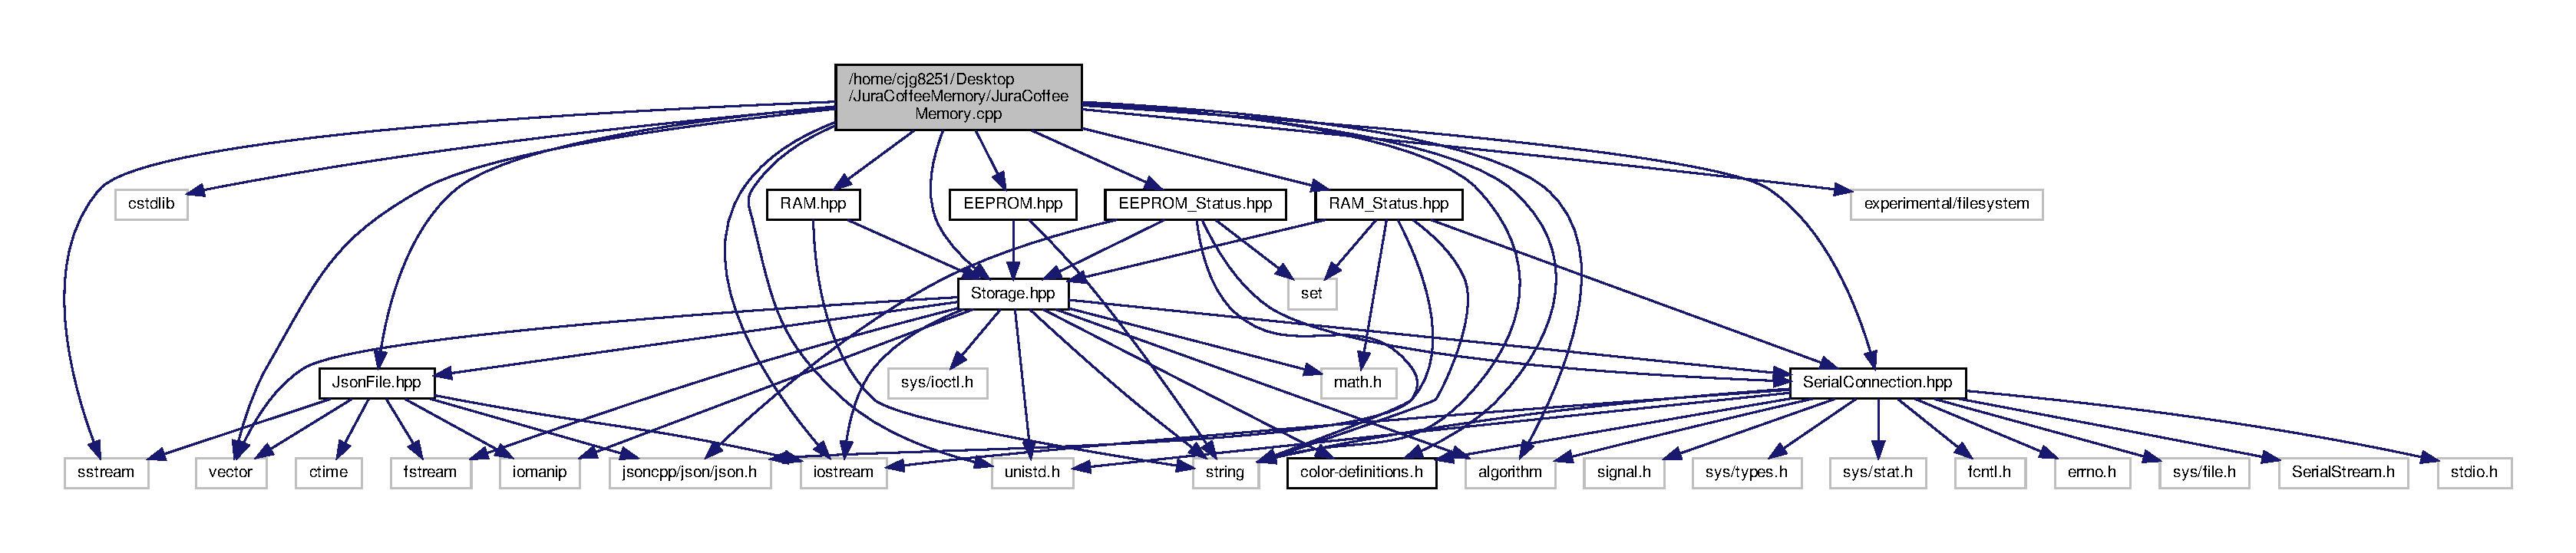
\includegraphics[width=350pt]{_jura_coffee_memory_8cpp__incl}
\end{center}
\end{figure}
\subsection*{Makrodefinitionen}
\begin{DoxyCompactItemize}
\item 
\#define \textbf{ O\+F\+F\+L\+I\+NE}~false
\end{DoxyCompactItemize}
\subsection*{Funktionen}
\begin{DoxyCompactItemize}
\item 
void \textbf{ eeprom} (string \&eeprom\+Path)
\item 
void \textbf{ ram} (string \&ram\+Path)
\item 
void \textbf{ Display\+Main\+Menu} ()
\item 
void \textbf{ Display\+Options\+Menu} (string \&device\+Path, string \&eeprom\+Path, string \&ram\+Path)
\item 
void \textbf{ Analyse\+File\+Dumps\+Menu} (string filename)
\item 
vector$<$ string $>$ \textbf{ Analyse\+Files\+List\+All} (string path)
\item 
void \textbf{ Analyse\+Files\+Menu} (string \&path)
\item 
void \textbf{ Options\+Menu} (string \&device\+Path, string \&eeprom\+Path, string \&ram\+Path)
\item 
void \textbf{ Main\+Menu} (string \&device\+Path, string \&path, string eeprom\+Path, string ram\+Path)
\item 
bool \textbf{ cmd\+Option\+Exists} (char $\ast$$\ast$begin, char $\ast$$\ast$end, const std\+::string \&option)
\item 
int \textbf{ main} (int argc, char $\ast$argv[$\,$])
\end{DoxyCompactItemize}


\subsection{Makro-\/\+Dokumentation}
\mbox{\label{_jura_coffee_memory_8cpp_a9fc595816a36e47d2b583afa775b3d4c}} 
\index{Jura\+Coffee\+Memory.\+cpp@{Jura\+Coffee\+Memory.\+cpp}!O\+F\+F\+L\+I\+NE@{O\+F\+F\+L\+I\+NE}}
\index{O\+F\+F\+L\+I\+NE@{O\+F\+F\+L\+I\+NE}!Jura\+Coffee\+Memory.\+cpp@{Jura\+Coffee\+Memory.\+cpp}}
\subsubsection{O\+F\+F\+L\+I\+NE}
{\footnotesize\ttfamily \#define O\+F\+F\+L\+I\+NE~false}



\subsection{Dokumentation der Funktionen}
\mbox{\label{_jura_coffee_memory_8cpp_ab8bde046af6922695656d5315eb4850a}} 
\index{Jura\+Coffee\+Memory.\+cpp@{Jura\+Coffee\+Memory.\+cpp}!Analyse\+File\+Dumps\+Menu@{Analyse\+File\+Dumps\+Menu}}
\index{Analyse\+File\+Dumps\+Menu@{Analyse\+File\+Dumps\+Menu}!Jura\+Coffee\+Memory.\+cpp@{Jura\+Coffee\+Memory.\+cpp}}
\subsubsection{Analyse\+File\+Dumps\+Menu()}
{\footnotesize\ttfamily void Analyse\+File\+Dumps\+Menu (\begin{DoxyParamCaption}\item[{string}]{filename }\end{DoxyParamCaption})}

Hier ist ein Graph, der zeigt, was diese Funktion aufruft\+:
\nopagebreak
\begin{figure}[H]
\begin{center}
\leavevmode
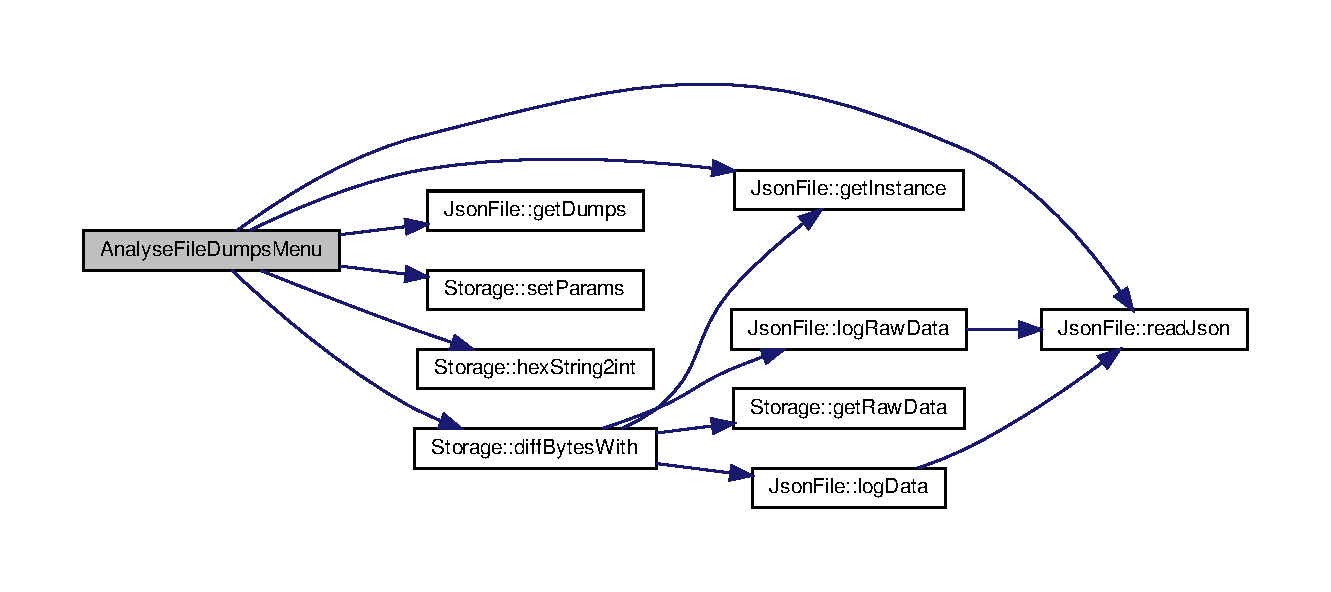
\includegraphics[width=350pt]{_jura_coffee_memory_8cpp_ab8bde046af6922695656d5315eb4850a_cgraph}
\end{center}
\end{figure}
\mbox{\label{_jura_coffee_memory_8cpp_af65003482ad2efc684f1bf59133d1b71}} 
\index{Jura\+Coffee\+Memory.\+cpp@{Jura\+Coffee\+Memory.\+cpp}!Analyse\+Files\+List\+All@{Analyse\+Files\+List\+All}}
\index{Analyse\+Files\+List\+All@{Analyse\+Files\+List\+All}!Jura\+Coffee\+Memory.\+cpp@{Jura\+Coffee\+Memory.\+cpp}}
\subsubsection{Analyse\+Files\+List\+All()}
{\footnotesize\ttfamily vector$<$string$>$ Analyse\+Files\+List\+All (\begin{DoxyParamCaption}\item[{string}]{path }\end{DoxyParamCaption})}

\mbox{\label{_jura_coffee_memory_8cpp_a755b1b20dcd140974d1760d5d19efbae}} 
\index{Jura\+Coffee\+Memory.\+cpp@{Jura\+Coffee\+Memory.\+cpp}!Analyse\+Files\+Menu@{Analyse\+Files\+Menu}}
\index{Analyse\+Files\+Menu@{Analyse\+Files\+Menu}!Jura\+Coffee\+Memory.\+cpp@{Jura\+Coffee\+Memory.\+cpp}}
\subsubsection{Analyse\+Files\+Menu()}
{\footnotesize\ttfamily void Analyse\+Files\+Menu (\begin{DoxyParamCaption}\item[{string \&}]{path }\end{DoxyParamCaption})}

Hier ist ein Graph, der zeigt, was diese Funktion aufruft\+:
\nopagebreak
\begin{figure}[H]
\begin{center}
\leavevmode
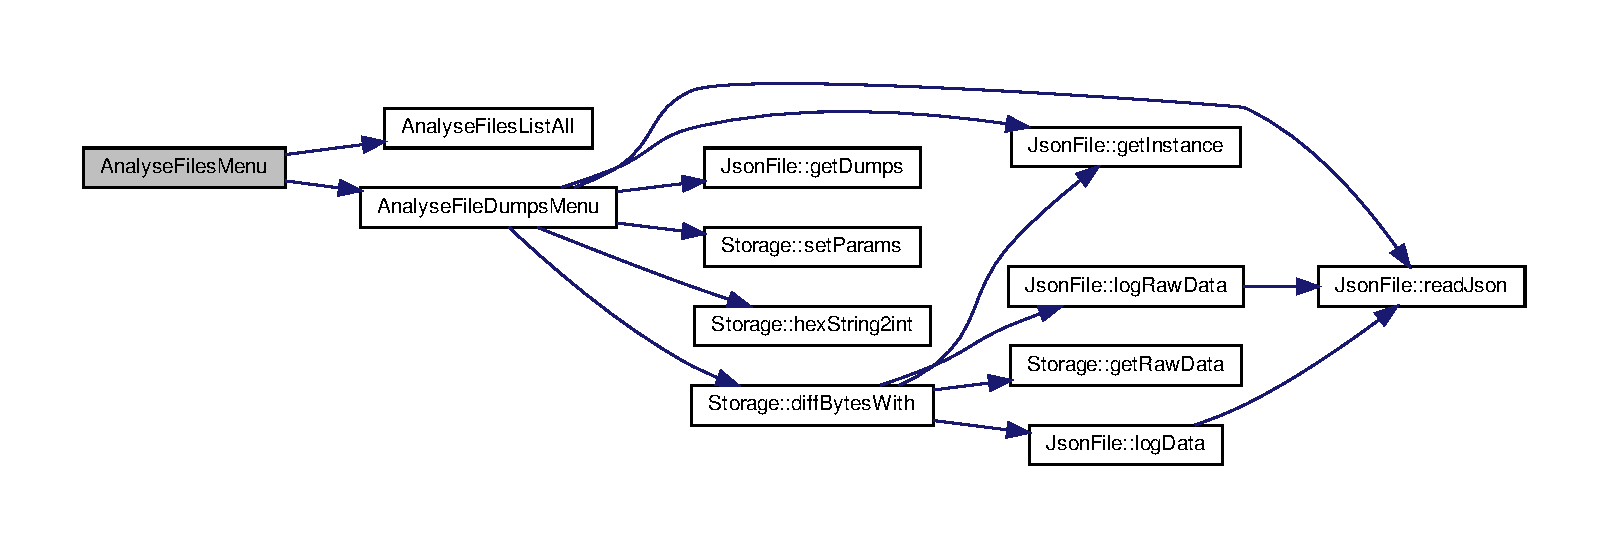
\includegraphics[width=350pt]{_jura_coffee_memory_8cpp_a755b1b20dcd140974d1760d5d19efbae_cgraph}
\end{center}
\end{figure}
\mbox{\label{_jura_coffee_memory_8cpp_a3e17e291195c7153863766f9374c14ab}} 
\index{Jura\+Coffee\+Memory.\+cpp@{Jura\+Coffee\+Memory.\+cpp}!cmd\+Option\+Exists@{cmd\+Option\+Exists}}
\index{cmd\+Option\+Exists@{cmd\+Option\+Exists}!Jura\+Coffee\+Memory.\+cpp@{Jura\+Coffee\+Memory.\+cpp}}
\subsubsection{cmd\+Option\+Exists()}
{\footnotesize\ttfamily bool cmd\+Option\+Exists (\begin{DoxyParamCaption}\item[{char $\ast$$\ast$}]{begin,  }\item[{char $\ast$$\ast$}]{end,  }\item[{const std\+::string \&}]{option }\end{DoxyParamCaption})}

\mbox{\label{_jura_coffee_memory_8cpp_a9801ee1f612b606462a61b77cef5ac94}} 
\index{Jura\+Coffee\+Memory.\+cpp@{Jura\+Coffee\+Memory.\+cpp}!Display\+Main\+Menu@{Display\+Main\+Menu}}
\index{Display\+Main\+Menu@{Display\+Main\+Menu}!Jura\+Coffee\+Memory.\+cpp@{Jura\+Coffee\+Memory.\+cpp}}
\subsubsection{Display\+Main\+Menu()}
{\footnotesize\ttfamily void Display\+Main\+Menu (\begin{DoxyParamCaption}{ }\end{DoxyParamCaption})}

\mbox{\label{_jura_coffee_memory_8cpp_a97c243c8048c19a393f1e73c92af4918}} 
\index{Jura\+Coffee\+Memory.\+cpp@{Jura\+Coffee\+Memory.\+cpp}!Display\+Options\+Menu@{Display\+Options\+Menu}}
\index{Display\+Options\+Menu@{Display\+Options\+Menu}!Jura\+Coffee\+Memory.\+cpp@{Jura\+Coffee\+Memory.\+cpp}}
\subsubsection{Display\+Options\+Menu()}
{\footnotesize\ttfamily void Display\+Options\+Menu (\begin{DoxyParamCaption}\item[{string \&}]{device\+Path,  }\item[{string \&}]{eeprom\+Path,  }\item[{string \&}]{ram\+Path }\end{DoxyParamCaption})}

\mbox{\label{_jura_coffee_memory_8cpp_a7f8b7f6e1e79a9ca640e51eb5aea9127}} 
\index{Jura\+Coffee\+Memory.\+cpp@{Jura\+Coffee\+Memory.\+cpp}!eeprom@{eeprom}}
\index{eeprom@{eeprom}!Jura\+Coffee\+Memory.\+cpp@{Jura\+Coffee\+Memory.\+cpp}}
\subsubsection{eeprom()}
{\footnotesize\ttfamily void eeprom (\begin{DoxyParamCaption}\item[{string \&}]{eeprom\+Path }\end{DoxyParamCaption})}

Hier ist ein Graph, der zeigt, was diese Funktion aufruft\+:
\nopagebreak
\begin{figure}[H]
\begin{center}
\leavevmode
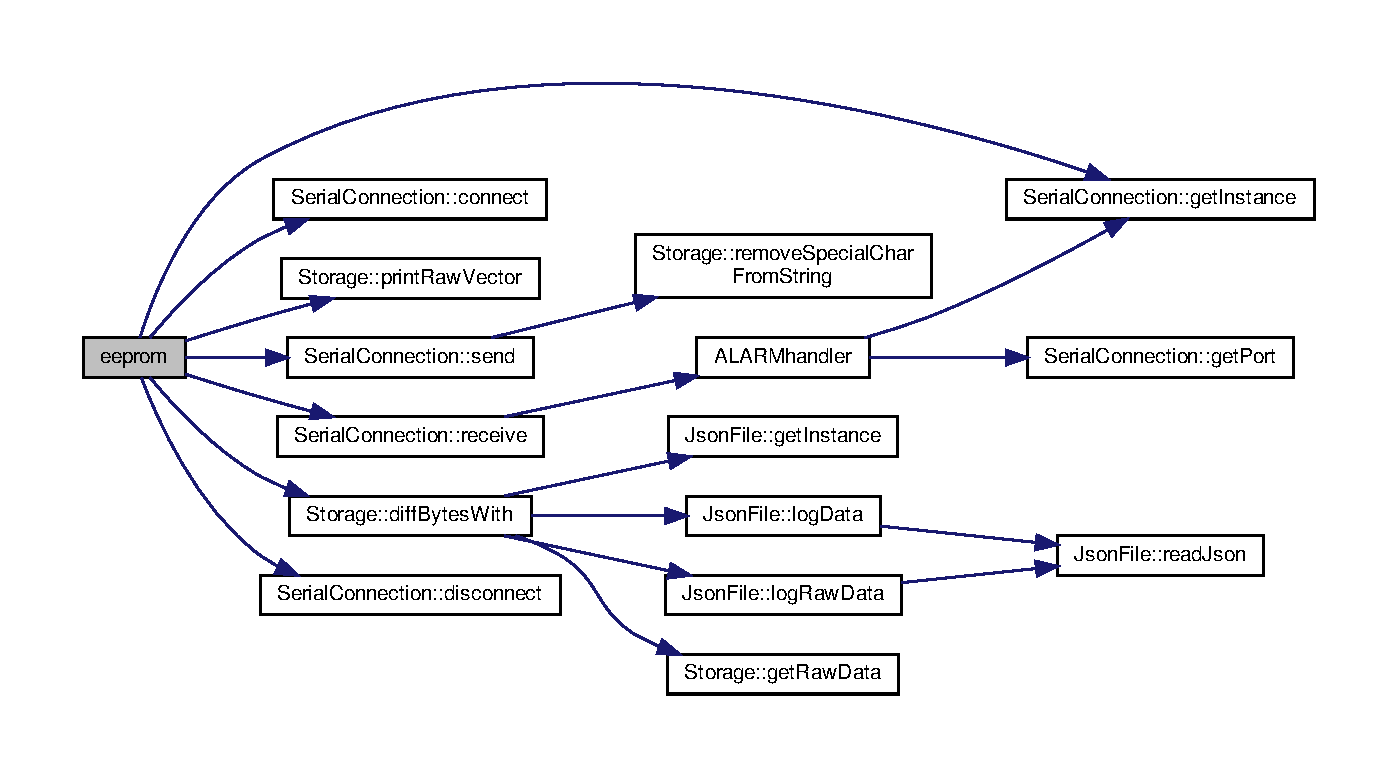
\includegraphics[width=350pt]{_jura_coffee_memory_8cpp_a7f8b7f6e1e79a9ca640e51eb5aea9127_cgraph}
\end{center}
\end{figure}
\mbox{\label{_jura_coffee_memory_8cpp_a0ddf1224851353fc92bfbff6f499fa97}} 
\index{Jura\+Coffee\+Memory.\+cpp@{Jura\+Coffee\+Memory.\+cpp}!main@{main}}
\index{main@{main}!Jura\+Coffee\+Memory.\+cpp@{Jura\+Coffee\+Memory.\+cpp}}
\subsubsection{main()}
{\footnotesize\ttfamily int main (\begin{DoxyParamCaption}\item[{int}]{argc,  }\item[{char $\ast$}]{argv[$\,$] }\end{DoxyParamCaption})}

Hier ist ein Graph, der zeigt, was diese Funktion aufruft\+:
\nopagebreak
\begin{figure}[H]
\begin{center}
\leavevmode
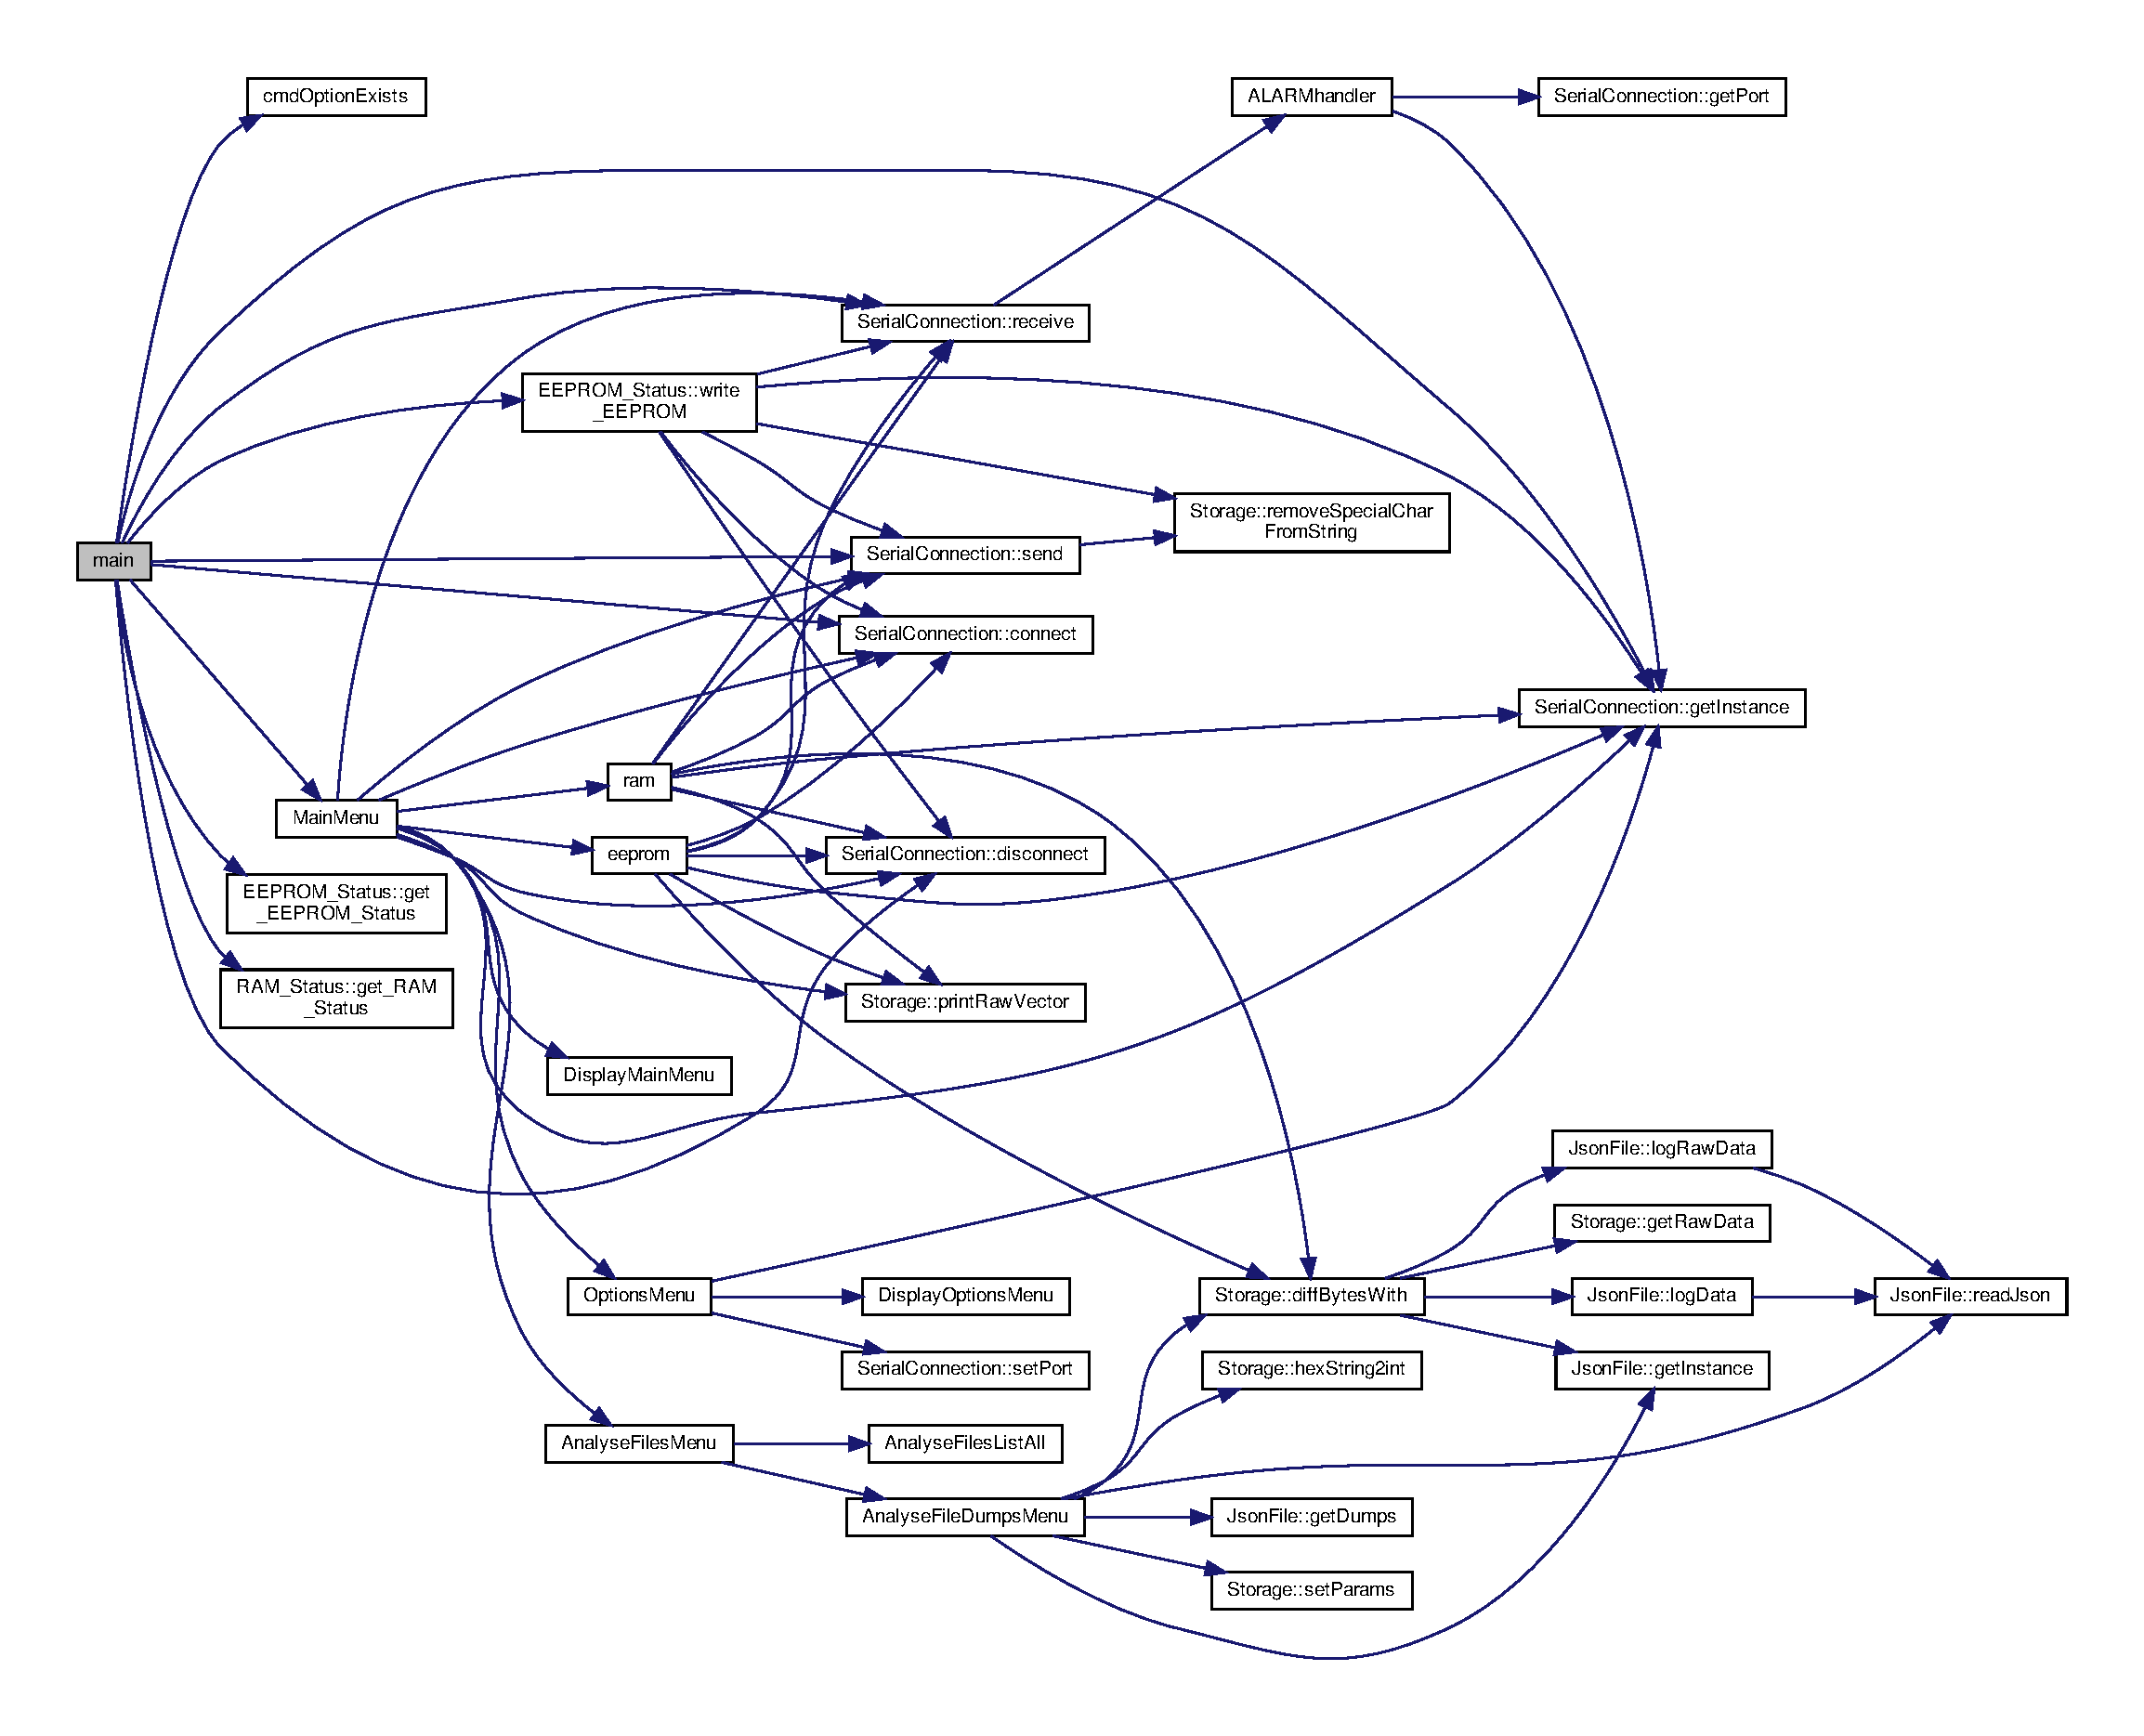
\includegraphics[width=350pt]{_jura_coffee_memory_8cpp_a0ddf1224851353fc92bfbff6f499fa97_cgraph}
\end{center}
\end{figure}
\mbox{\label{_jura_coffee_memory_8cpp_a738ac361f7823bd523c2b86533ed2b67}} 
\index{Jura\+Coffee\+Memory.\+cpp@{Jura\+Coffee\+Memory.\+cpp}!Main\+Menu@{Main\+Menu}}
\index{Main\+Menu@{Main\+Menu}!Jura\+Coffee\+Memory.\+cpp@{Jura\+Coffee\+Memory.\+cpp}}
\subsubsection{Main\+Menu()}
{\footnotesize\ttfamily void Main\+Menu (\begin{DoxyParamCaption}\item[{string \&}]{device\+Path,  }\item[{string \&}]{path,  }\item[{string}]{eeprom\+Path,  }\item[{string}]{ram\+Path }\end{DoxyParamCaption})}

Hier ist ein Graph, der zeigt, was diese Funktion aufruft\+:
\nopagebreak
\begin{figure}[H]
\begin{center}
\leavevmode
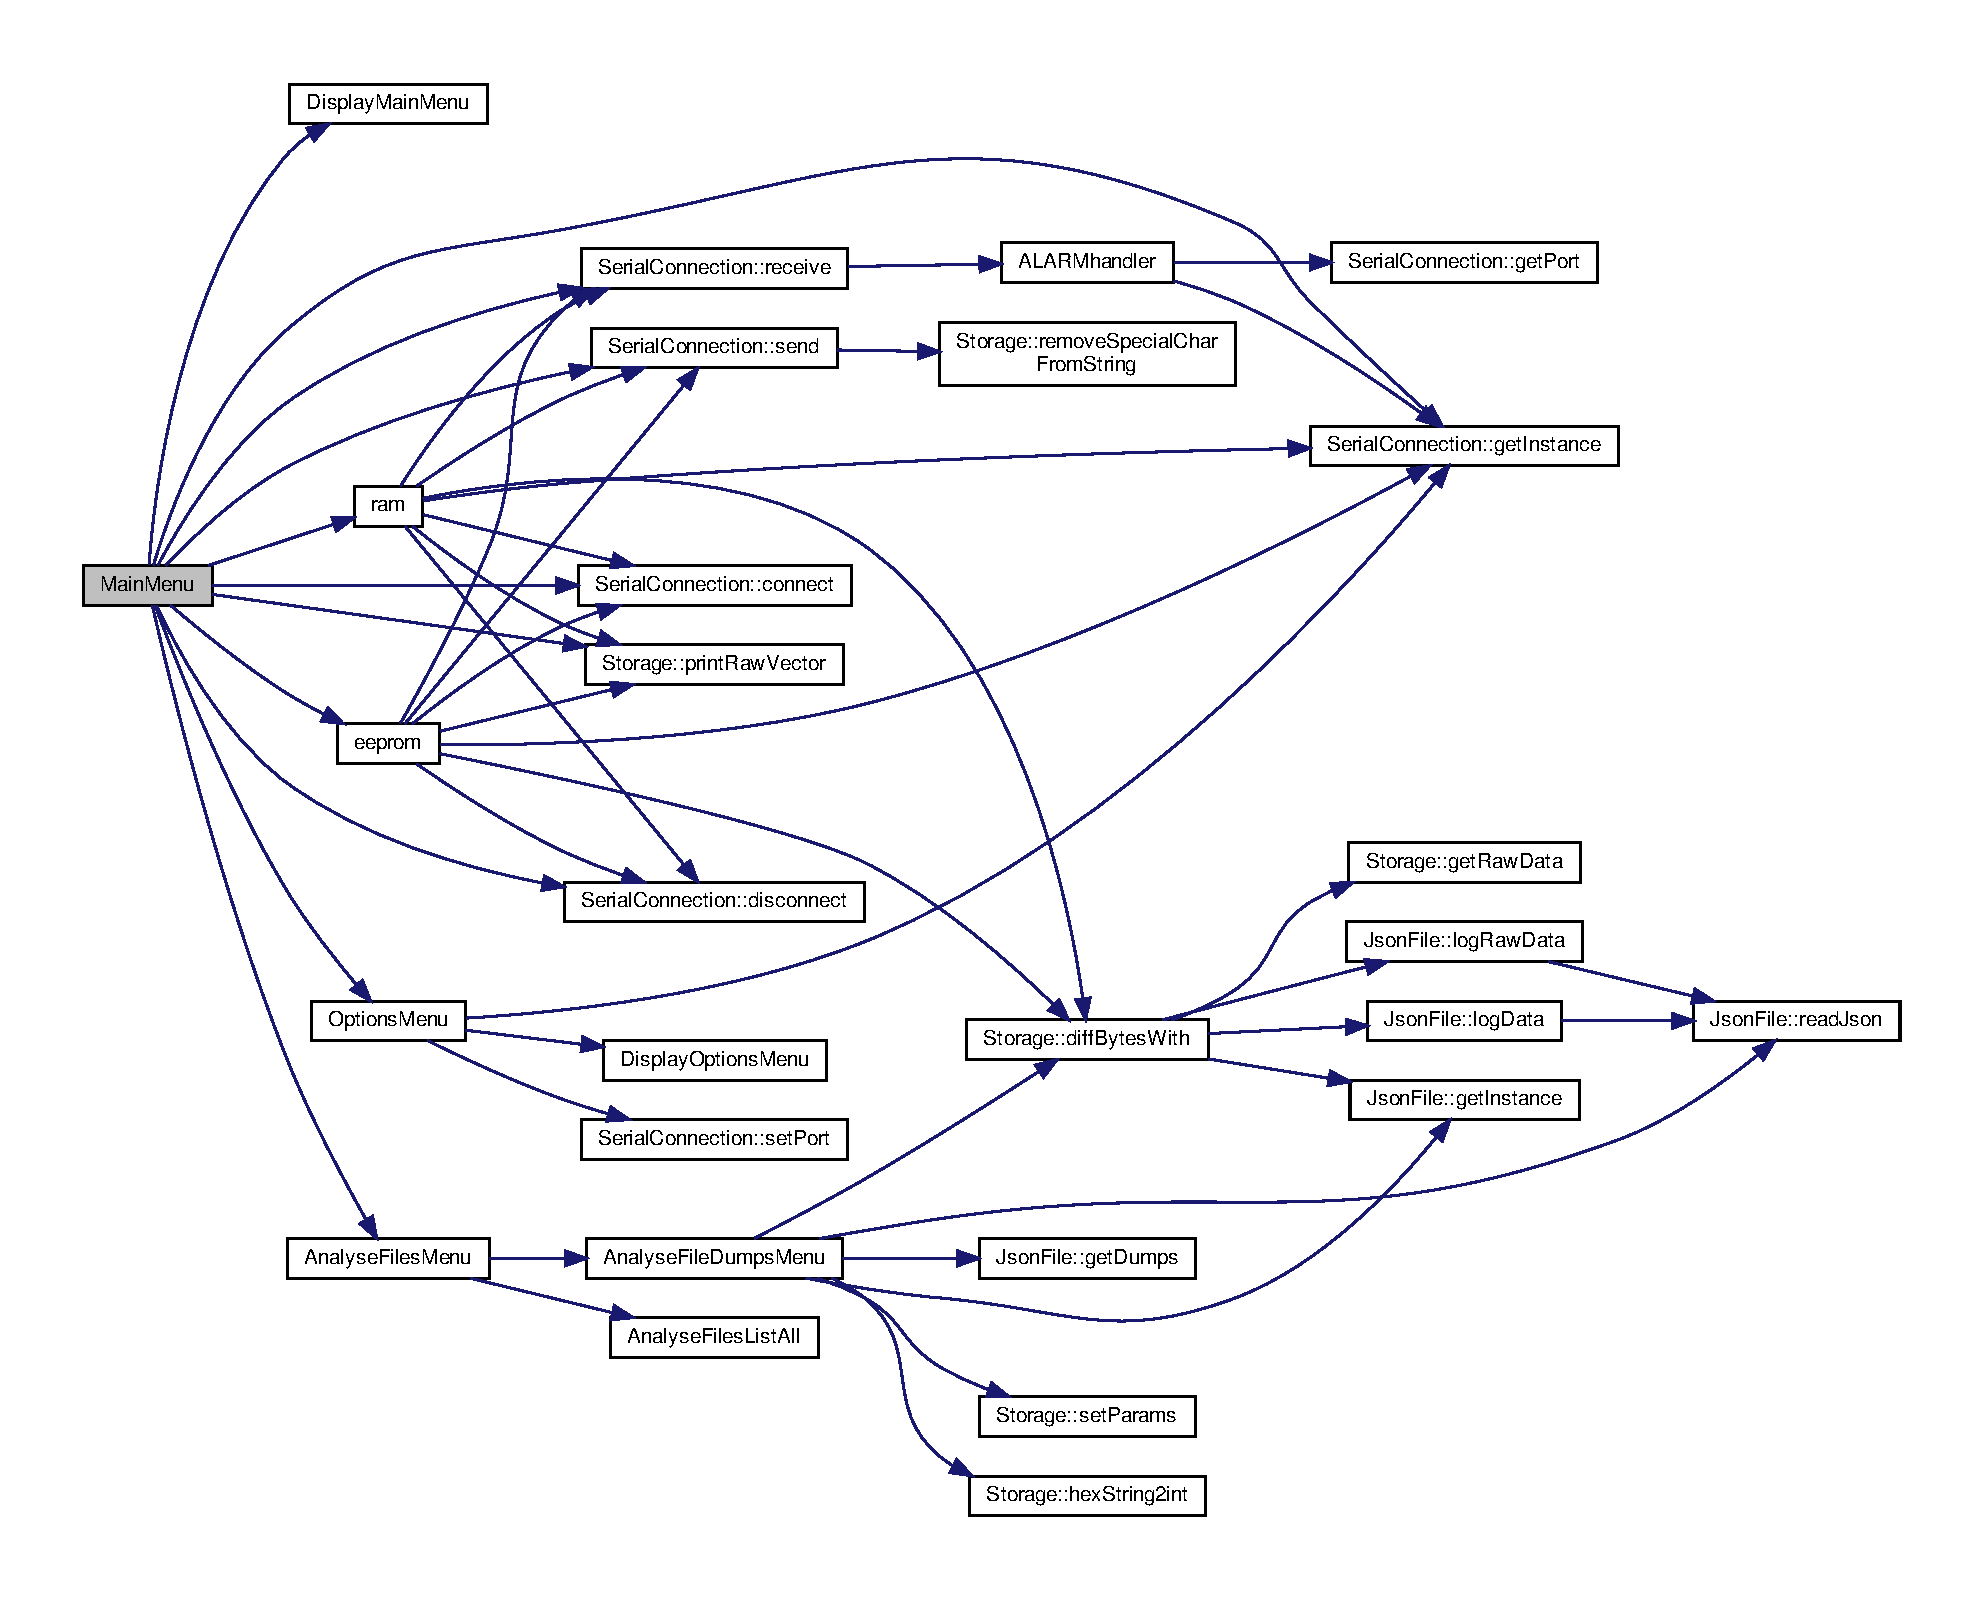
\includegraphics[width=350pt]{_jura_coffee_memory_8cpp_a738ac361f7823bd523c2b86533ed2b67_cgraph}
\end{center}
\end{figure}
\mbox{\label{_jura_coffee_memory_8cpp_ae46c8e2155f07fd7da805fc23e7778ad}} 
\index{Jura\+Coffee\+Memory.\+cpp@{Jura\+Coffee\+Memory.\+cpp}!Options\+Menu@{Options\+Menu}}
\index{Options\+Menu@{Options\+Menu}!Jura\+Coffee\+Memory.\+cpp@{Jura\+Coffee\+Memory.\+cpp}}
\subsubsection{Options\+Menu()}
{\footnotesize\ttfamily void Options\+Menu (\begin{DoxyParamCaption}\item[{string \&}]{device\+Path,  }\item[{string \&}]{eeprom\+Path,  }\item[{string \&}]{ram\+Path }\end{DoxyParamCaption})}

Hier ist ein Graph, der zeigt, was diese Funktion aufruft\+:
\nopagebreak
\begin{figure}[H]
\begin{center}
\leavevmode
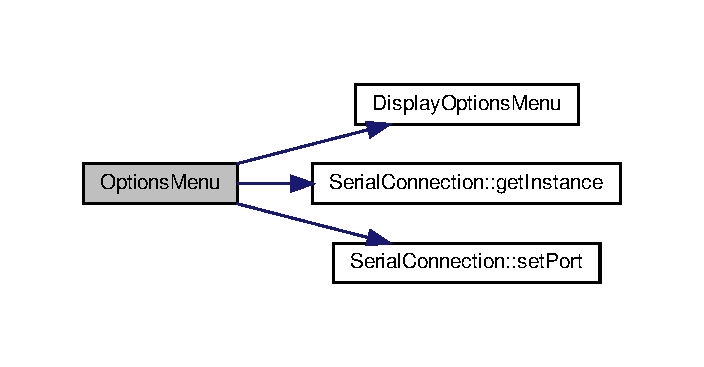
\includegraphics[width=338pt]{_jura_coffee_memory_8cpp_ae46c8e2155f07fd7da805fc23e7778ad_cgraph}
\end{center}
\end{figure}
\mbox{\label{_jura_coffee_memory_8cpp_affa74aeb23b81d2c3e06941867347bd8}} 
\index{Jura\+Coffee\+Memory.\+cpp@{Jura\+Coffee\+Memory.\+cpp}!ram@{ram}}
\index{ram@{ram}!Jura\+Coffee\+Memory.\+cpp@{Jura\+Coffee\+Memory.\+cpp}}
\subsubsection{ram()}
{\footnotesize\ttfamily void ram (\begin{DoxyParamCaption}\item[{string \&}]{ram\+Path }\end{DoxyParamCaption})}

Hier ist ein Graph, der zeigt, was diese Funktion aufruft\+:
\nopagebreak
\begin{figure}[H]
\begin{center}
\leavevmode
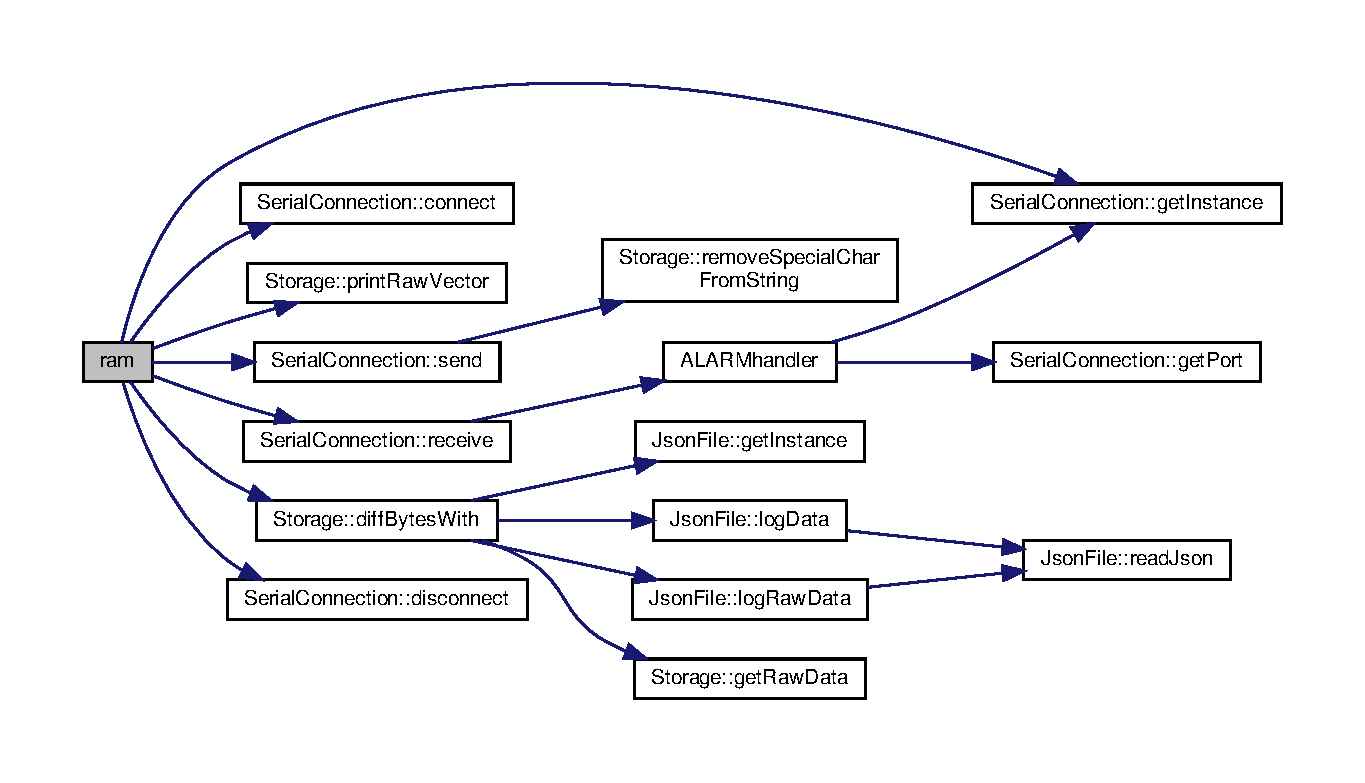
\includegraphics[width=350pt]{_jura_coffee_memory_8cpp_affa74aeb23b81d2c3e06941867347bd8_cgraph}
\end{center}
\end{figure}

\section{/home/cjg8251/\+Desktop/\+Jura\+Coffee\+Memory/\+R\+AM.cpp-\/\+Dateireferenz}
\label{_r_a_m_8cpp}\index{/home/cjg8251/\+Desktop/\+Jura\+Coffee\+Memory/\+R\+A\+M.\+cpp@{/home/cjg8251/\+Desktop/\+Jura\+Coffee\+Memory/\+R\+A\+M.\+cpp}}
{\ttfamily \#include \char`\"{}R\+A\+M.\+hpp\char`\"{}}\newline
Include-\/\+Abhängigkeitsdiagramm für R\+A\+M.\+cpp\+:
\nopagebreak
\begin{figure}[H]
\begin{center}
\leavevmode
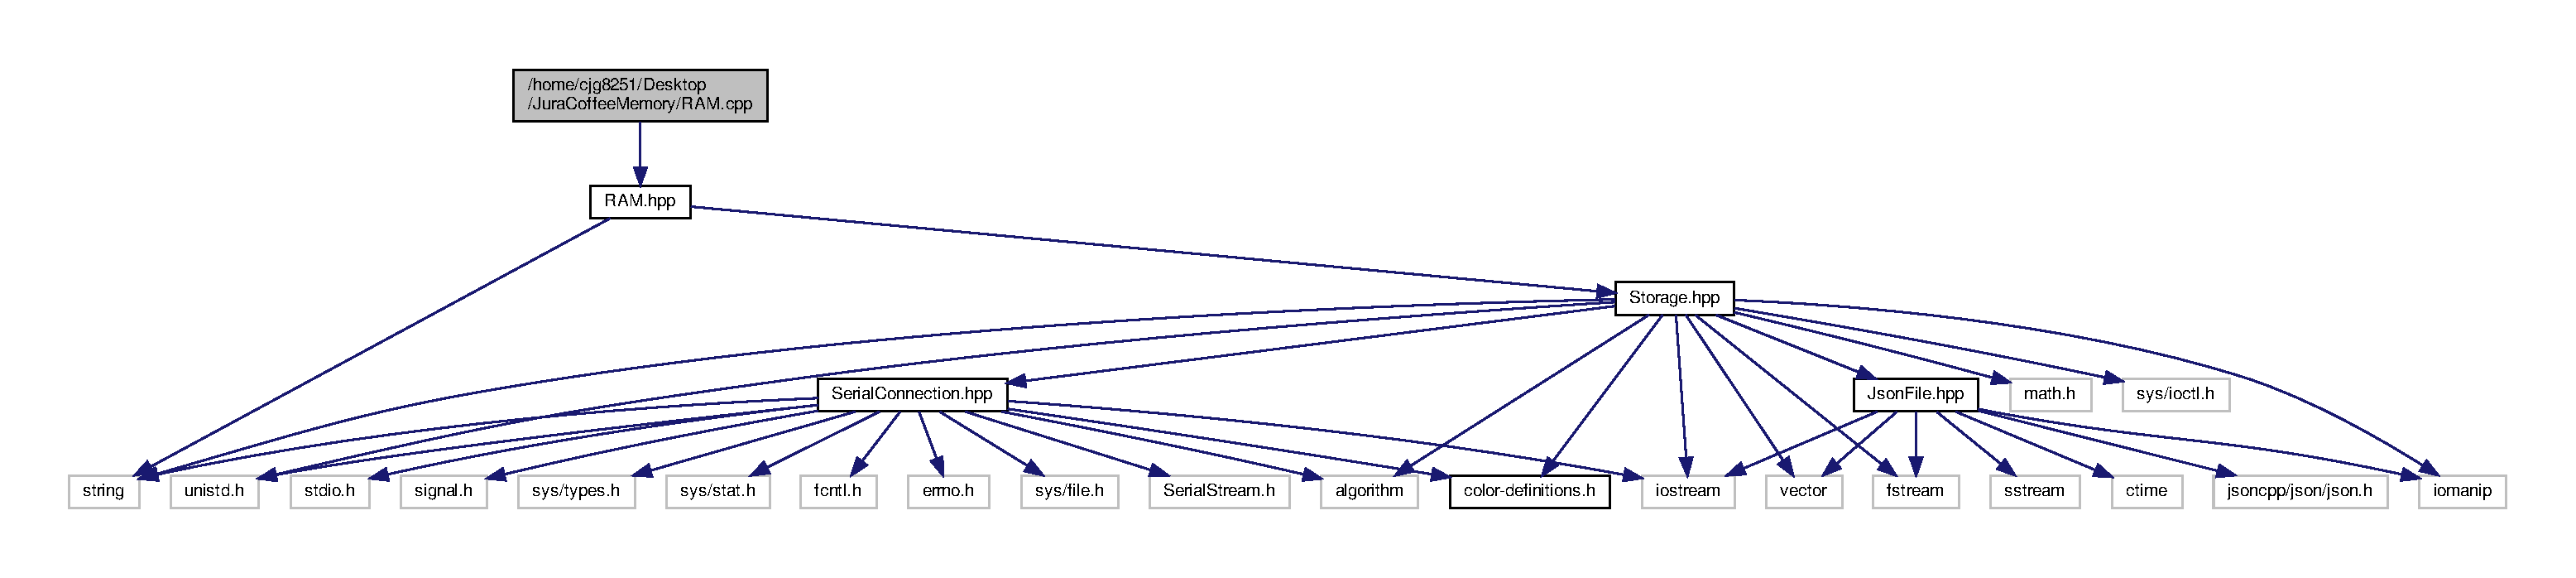
\includegraphics[width=350pt]{_r_a_m_8cpp__incl}
\end{center}
\end{figure}

\section{/home/cjg8251/\+Desktop/\+Jura\+Coffee\+Memory/\+R\+AM.hpp-\/\+Dateireferenz}
\label{_r_a_m_8hpp}\index{/home/cjg8251/\+Desktop/\+Jura\+Coffee\+Memory/\+R\+A\+M.\+hpp@{/home/cjg8251/\+Desktop/\+Jura\+Coffee\+Memory/\+R\+A\+M.\+hpp}}
{\ttfamily \#include $<$string$>$}\newline
{\ttfamily \#include \char`\"{}Storage.\+hpp\char`\"{}}\newline
Include-\/\+Abhängigkeitsdiagramm für R\+A\+M.\+hpp\+:
\nopagebreak
\begin{figure}[H]
\begin{center}
\leavevmode
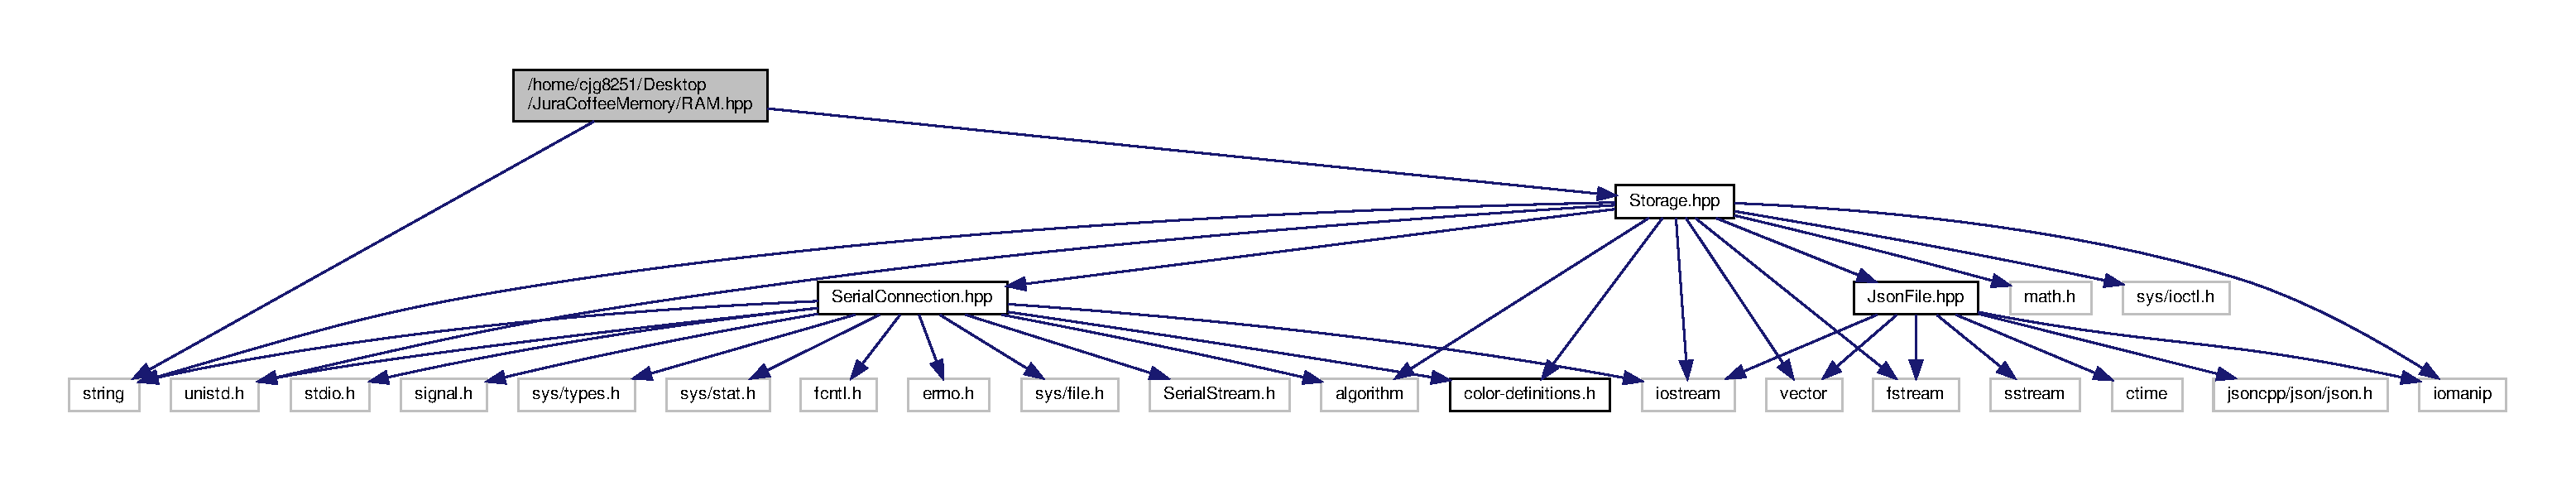
\includegraphics[width=350pt]{_r_a_m_8hpp__incl}
\end{center}
\end{figure}
Dieser Graph zeigt, welche Datei direkt oder indirekt diese Datei enthält\+:
\nopagebreak
\begin{figure}[H]
\begin{center}
\leavevmode
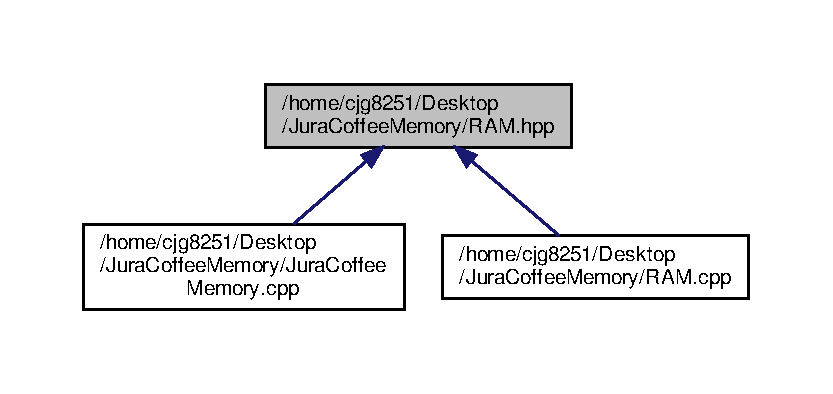
\includegraphics[width=350pt]{_r_a_m_8hpp__dep__incl}
\end{center}
\end{figure}
\subsection*{Klassen}
\begin{DoxyCompactItemize}
\item 
class \textbf{ R\+AM}
\end{DoxyCompactItemize}

\section{/home/cjg8251/\+Desktop/\+Jura\+Coffee\+Memory/\+R\+A\+M\+\_\+\+Status.cpp-\/\+Dateireferenz}
\label{_r_a_m___status_8cpp}\index{/home/cjg8251/\+Desktop/\+Jura\+Coffee\+Memory/\+R\+A\+M\+\_\+\+Status.\+cpp@{/home/cjg8251/\+Desktop/\+Jura\+Coffee\+Memory/\+R\+A\+M\+\_\+\+Status.\+cpp}}
{\ttfamily \#include \char`\"{}R\+A\+M\+\_\+\+Status.\+hpp\char`\"{}}\newline
Include-\/\+Abhängigkeitsdiagramm für R\+A\+M\+\_\+\+Status.\+cpp\+:
\nopagebreak
\begin{figure}[H]
\begin{center}
\leavevmode
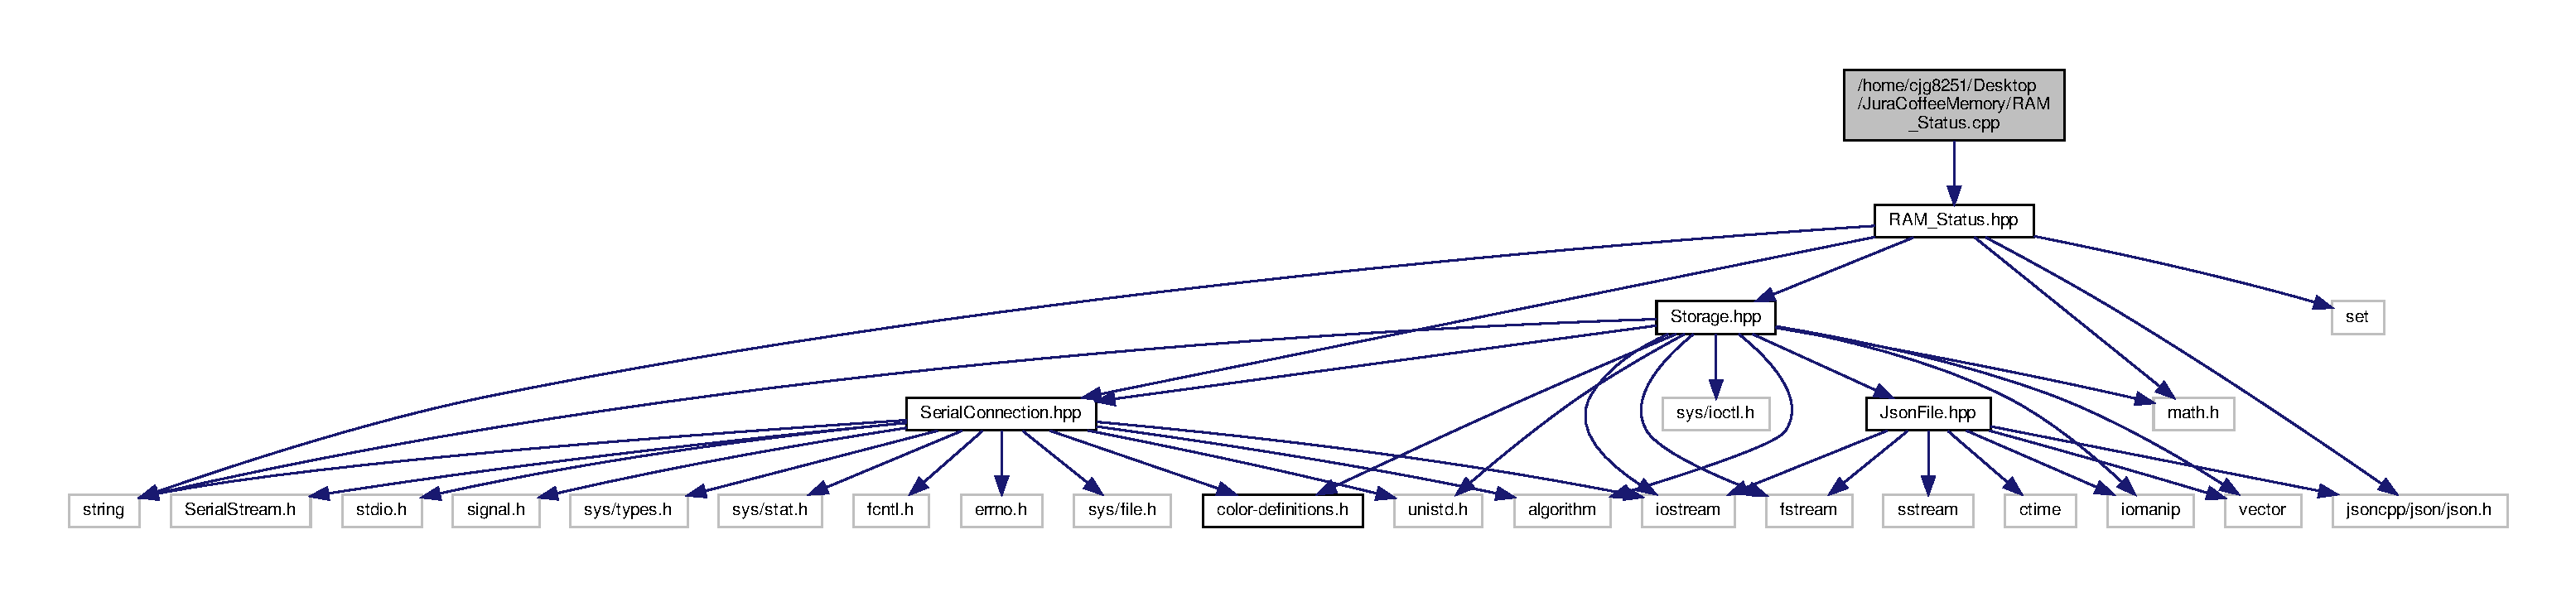
\includegraphics[width=350pt]{_r_a_m___status_8cpp__incl}
\end{center}
\end{figure}

\section{/home/cjg8251/\+Desktop/\+Jura\+Coffee\+Memory/\+R\+A\+M\+\_\+\+Status.hpp-\/\+Dateireferenz}
\label{_r_a_m___status_8hpp}\index{/home/cjg8251/\+Desktop/\+Jura\+Coffee\+Memory/\+R\+A\+M\+\_\+\+Status.\+hpp@{/home/cjg8251/\+Desktop/\+Jura\+Coffee\+Memory/\+R\+A\+M\+\_\+\+Status.\+hpp}}
{\ttfamily \#include $<$string$>$}\newline
{\ttfamily \#include $<$set$>$}\newline
{\ttfamily \#include \char`\"{}Storage.\+hpp\char`\"{}}\newline
{\ttfamily \#include \char`\"{}Serial\+Connection.\+hpp\char`\"{}}\newline
{\ttfamily \#include $<$jsoncpp/json/json.\+h$>$}\newline
{\ttfamily \#include $<$math.\+h$>$}\newline
Include-\/\+Abhängigkeitsdiagramm für R\+A\+M\+\_\+\+Status.\+hpp\+:
\nopagebreak
\begin{figure}[H]
\begin{center}
\leavevmode
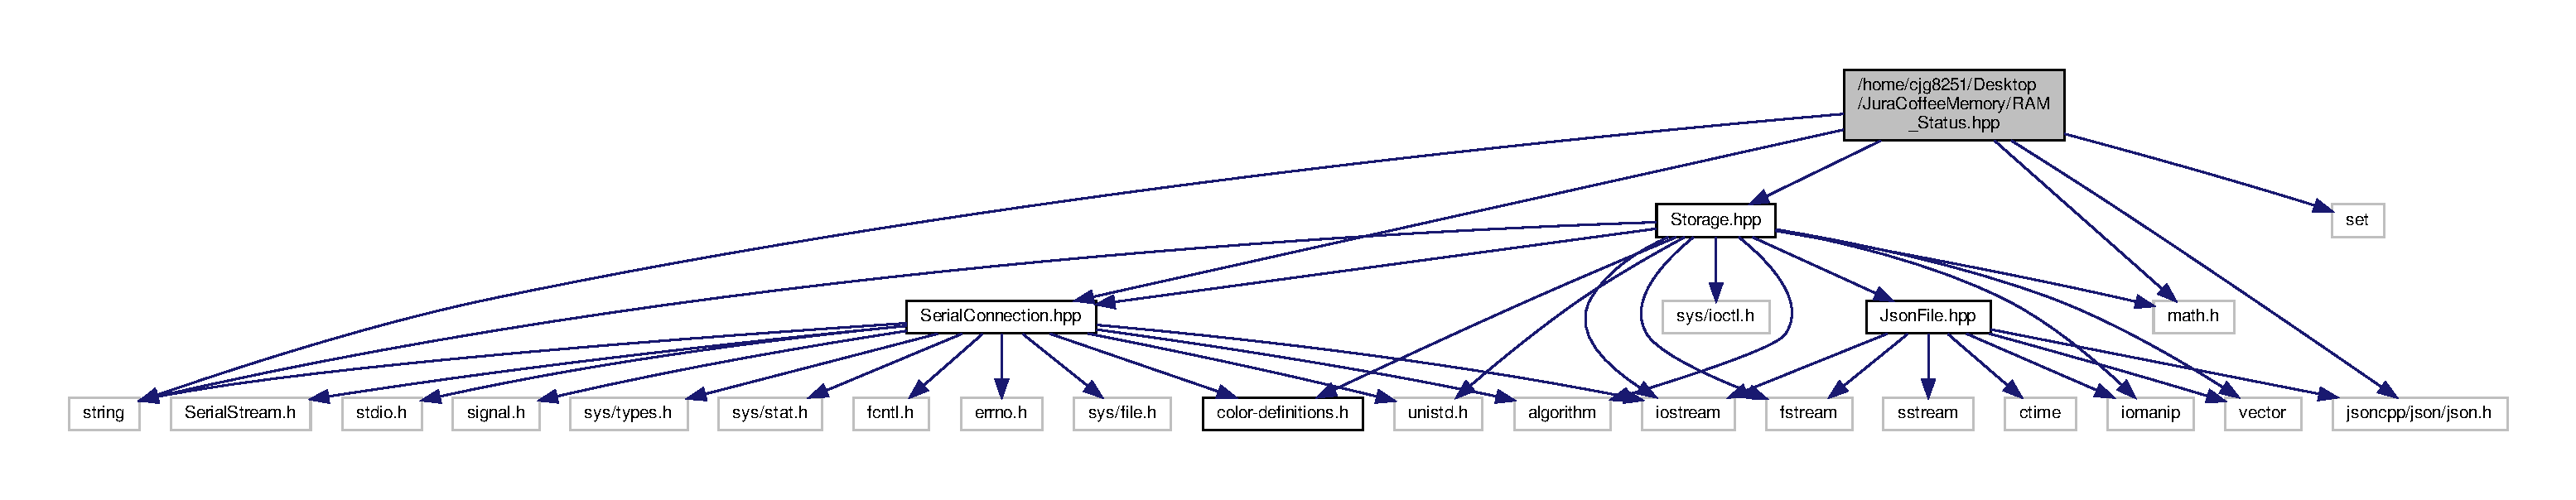
\includegraphics[width=350pt]{_r_a_m___status_8hpp__incl}
\end{center}
\end{figure}
Dieser Graph zeigt, welche Datei direkt oder indirekt diese Datei enthält\+:
\nopagebreak
\begin{figure}[H]
\begin{center}
\leavevmode
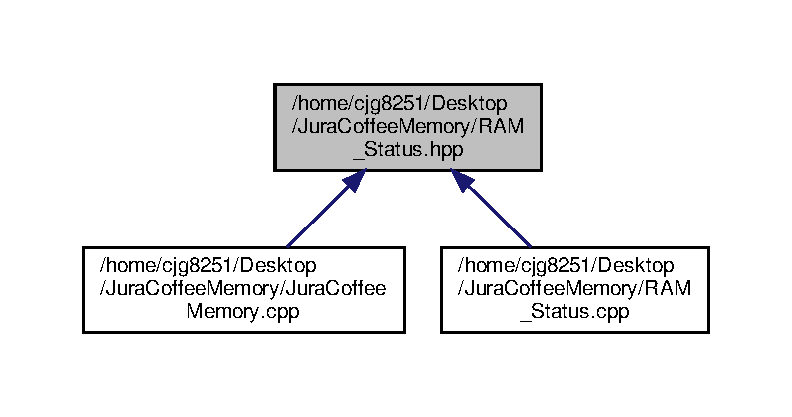
\includegraphics[width=350pt]{_r_a_m___status_8hpp__dep__incl}
\end{center}
\end{figure}
\subsection*{Klassen}
\begin{DoxyCompactItemize}
\item 
struct \textbf{ Entry\+R\+AM}
\item 
class \textbf{ R\+A\+M\+\_\+\+Status}
\end{DoxyCompactItemize}

\section{/home/cjg8251/\+Desktop/\+Jura\+Coffee\+Memory/\+Readme.md-\/\+Dateireferenz}
\label{_readme_8md}\index{/home/cjg8251/\+Desktop/\+Jura\+Coffee\+Memory/\+Readme.\+md@{/home/cjg8251/\+Desktop/\+Jura\+Coffee\+Memory/\+Readme.\+md}}

\section{/home/cjg8251/\+Desktop/\+Jura\+Coffee\+Memory/\+Serial\+Connection.cpp-\/\+Dateireferenz}
\label{_serial_connection_8cpp}\index{/home/cjg8251/\+Desktop/\+Jura\+Coffee\+Memory/\+Serial\+Connection.\+cpp@{/home/cjg8251/\+Desktop/\+Jura\+Coffee\+Memory/\+Serial\+Connection.\+cpp}}
{\ttfamily \#include \char`\"{}Serial\+Connection.\+hpp\char`\"{}}\newline
Include-\/\+Abhängigkeitsdiagramm für Serial\+Connection.\+cpp\+:
\nopagebreak
\begin{figure}[H]
\begin{center}
\leavevmode
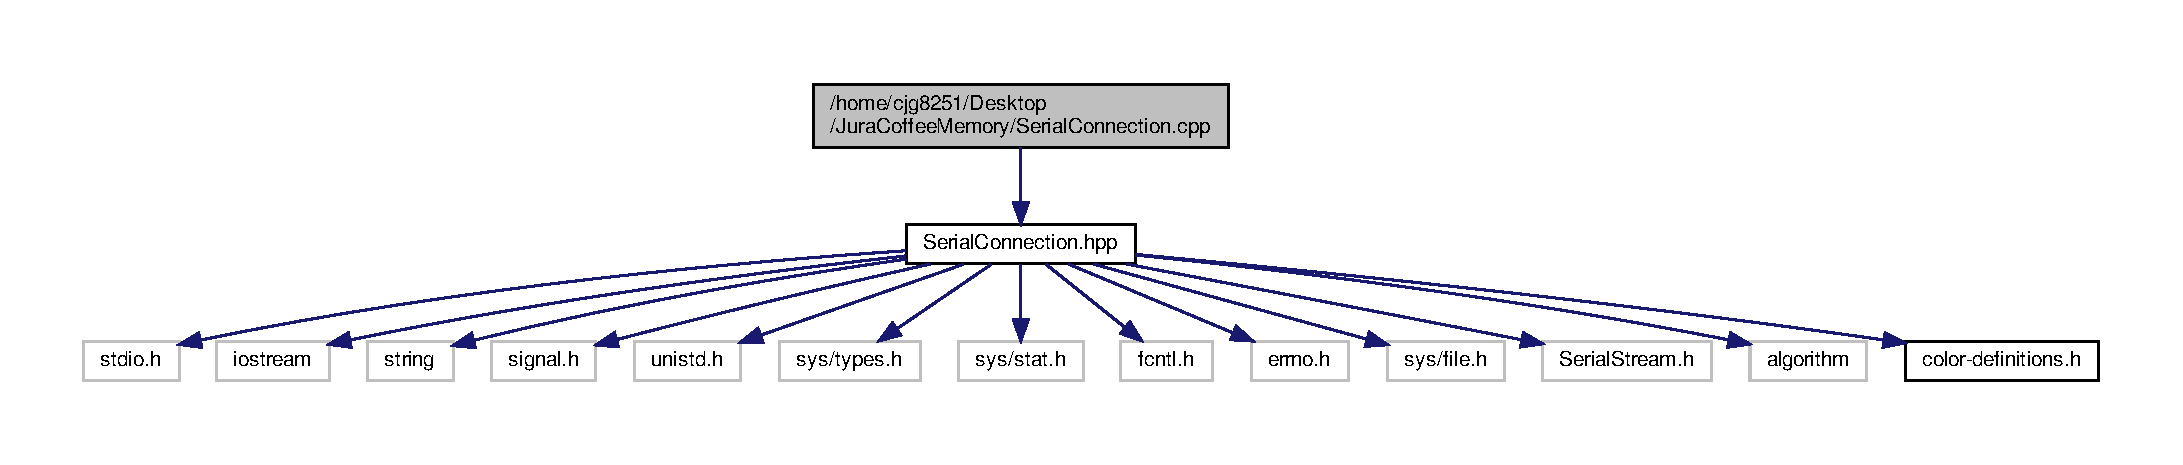
\includegraphics[width=350pt]{_serial_connection_8cpp__incl}
\end{center}
\end{figure}
\subsection*{Funktionen}
\begin{DoxyCompactItemize}
\item 
void \textbf{ A\+L\+A\+R\+Mhandler} (int sig)
\end{DoxyCompactItemize}


\subsection{Dokumentation der Funktionen}
\mbox{\label{_serial_connection_8cpp_a1e8896b6fa0aa733d2fdb7a3a3891a3b}} 
\index{Serial\+Connection.\+cpp@{Serial\+Connection.\+cpp}!A\+L\+A\+R\+Mhandler@{A\+L\+A\+R\+Mhandler}}
\index{A\+L\+A\+R\+Mhandler@{A\+L\+A\+R\+Mhandler}!Serial\+Connection.\+cpp@{Serial\+Connection.\+cpp}}
\subsubsection{A\+L\+A\+R\+Mhandler()}
{\footnotesize\ttfamily void A\+L\+A\+R\+Mhandler (\begin{DoxyParamCaption}\item[{int}]{sig }\end{DoxyParamCaption})}

Hier ist ein Graph, der zeigt, was diese Funktion aufruft\+:\nopagebreak
\begin{figure}[H]
\begin{center}
\leavevmode
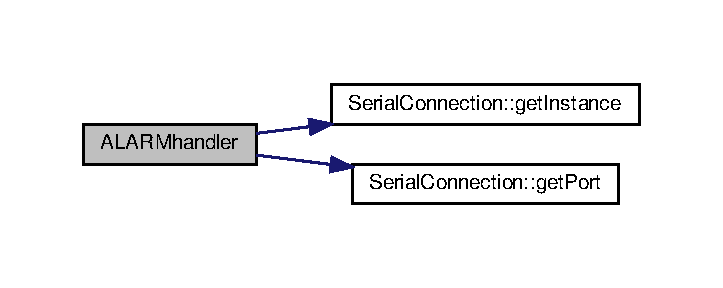
\includegraphics[width=347pt]{_serial_connection_8cpp_a1e8896b6fa0aa733d2fdb7a3a3891a3b_cgraph}
\end{center}
\end{figure}

\section{/home/cjg8251/\+Desktop/\+Jura\+Coffee\+Memory/\+Serial\+Connection.hpp-\/\+Dateireferenz}
\label{_serial_connection_8hpp}\index{/home/cjg8251/\+Desktop/\+Jura\+Coffee\+Memory/\+Serial\+Connection.\+hpp@{/home/cjg8251/\+Desktop/\+Jura\+Coffee\+Memory/\+Serial\+Connection.\+hpp}}
{\ttfamily \#include $<$stdio.\+h$>$}\newline
{\ttfamily \#include $<$iostream$>$}\newline
{\ttfamily \#include $<$string$>$}\newline
{\ttfamily \#include $<$signal.\+h$>$}\newline
{\ttfamily \#include $<$unistd.\+h$>$}\newline
{\ttfamily \#include $<$sys/types.\+h$>$}\newline
{\ttfamily \#include $<$sys/stat.\+h$>$}\newline
{\ttfamily \#include $<$fcntl.\+h$>$}\newline
{\ttfamily \#include $<$errno.\+h$>$}\newline
{\ttfamily \#include $<$sys/file.\+h$>$}\newline
{\ttfamily \#include $<$Serial\+Stream.\+h$>$}\newline
{\ttfamily \#include $<$algorithm$>$}\newline
{\ttfamily \#include \char`\"{}color-\/definitions.\+h\char`\"{}}\newline
Include-\/\+Abhängigkeitsdiagramm für Serial\+Connection.\+hpp\+:
\nopagebreak
\begin{figure}[H]
\begin{center}
\leavevmode
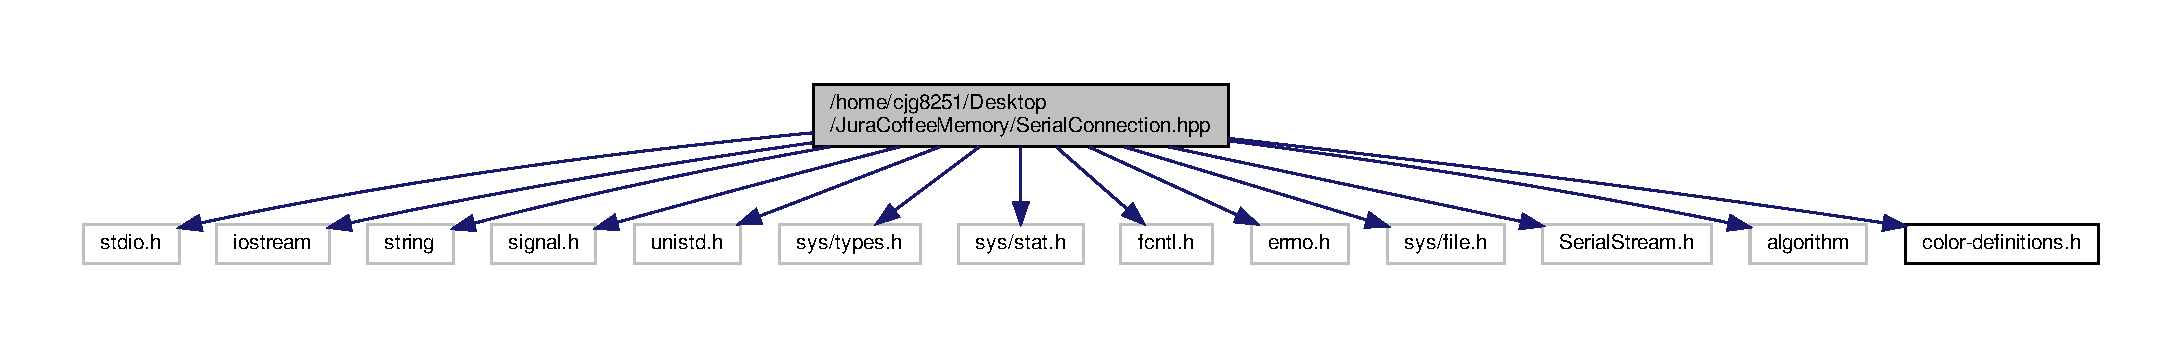
\includegraphics[width=350pt]{_serial_connection_8hpp__incl}
\end{center}
\end{figure}
Dieser Graph zeigt, welche Datei direkt oder indirekt diese Datei enthält\+:
\nopagebreak
\begin{figure}[H]
\begin{center}
\leavevmode
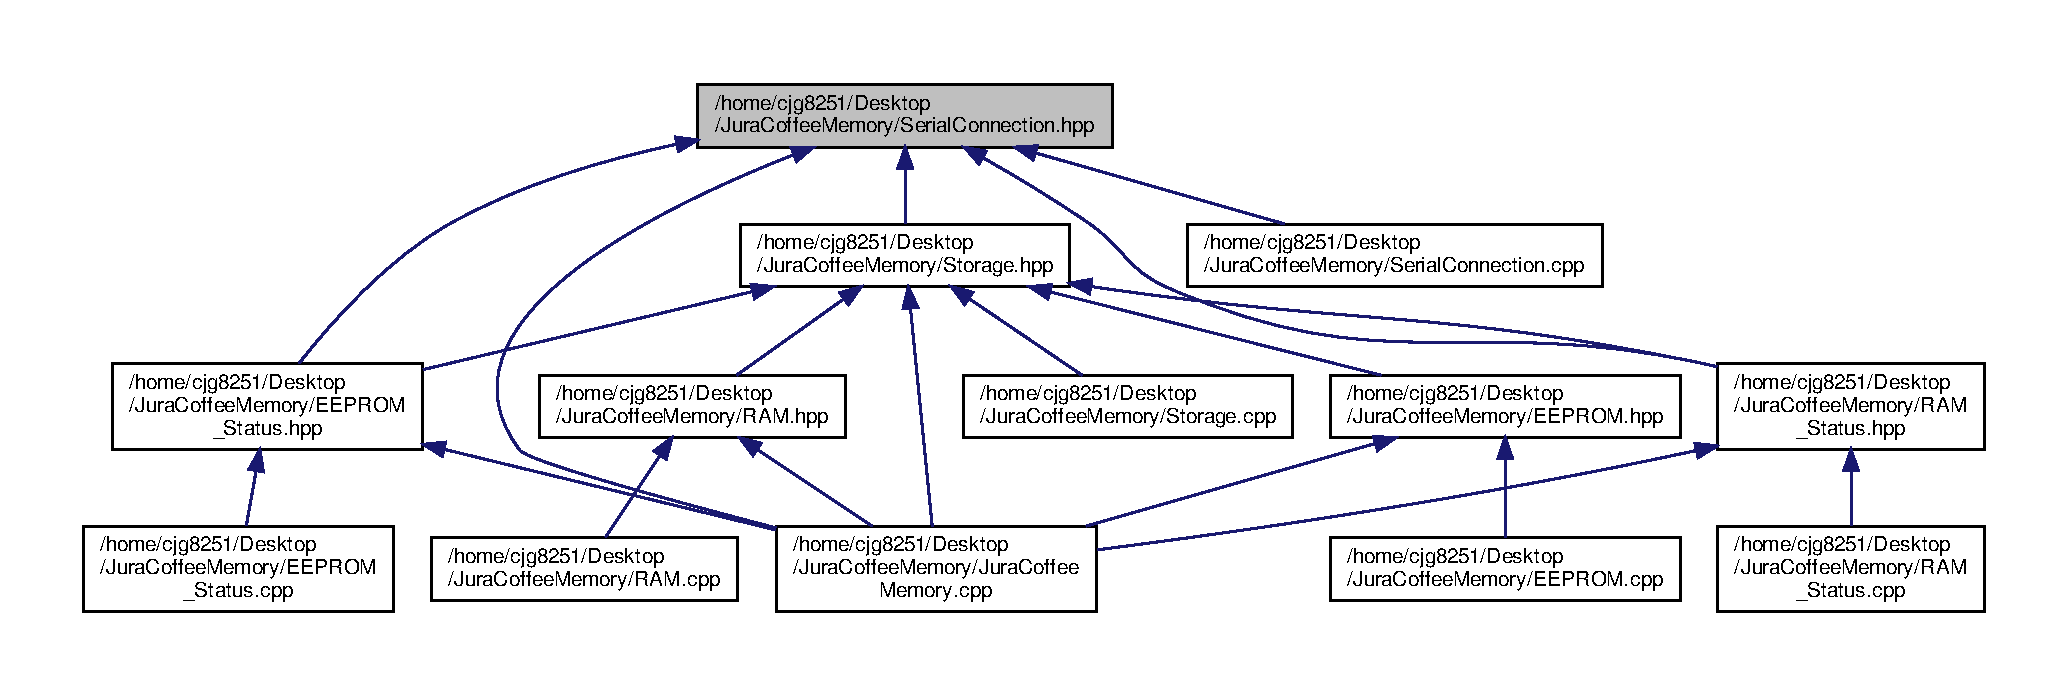
\includegraphics[width=350pt]{_serial_connection_8hpp__dep__incl}
\end{center}
\end{figure}
\subsection*{Klassen}
\begin{DoxyCompactItemize}
\item 
class \textbf{ Serial\+Connection}
\end{DoxyCompactItemize}

\section{/home/cjg8251/\+Desktop/\+Jura\+Coffee\+Memory/\+Storage.cpp-\/\+Dateireferenz}
\label{_storage_8cpp}\index{/home/cjg8251/\+Desktop/\+Jura\+Coffee\+Memory/\+Storage.\+cpp@{/home/cjg8251/\+Desktop/\+Jura\+Coffee\+Memory/\+Storage.\+cpp}}
{\ttfamily \#include \char`\"{}Storage.\+hpp\char`\"{}}\newline
Include-\/\+Abhängigkeitsdiagramm für Storage.\+cpp\+:
\nopagebreak
\begin{figure}[H]
\begin{center}
\leavevmode
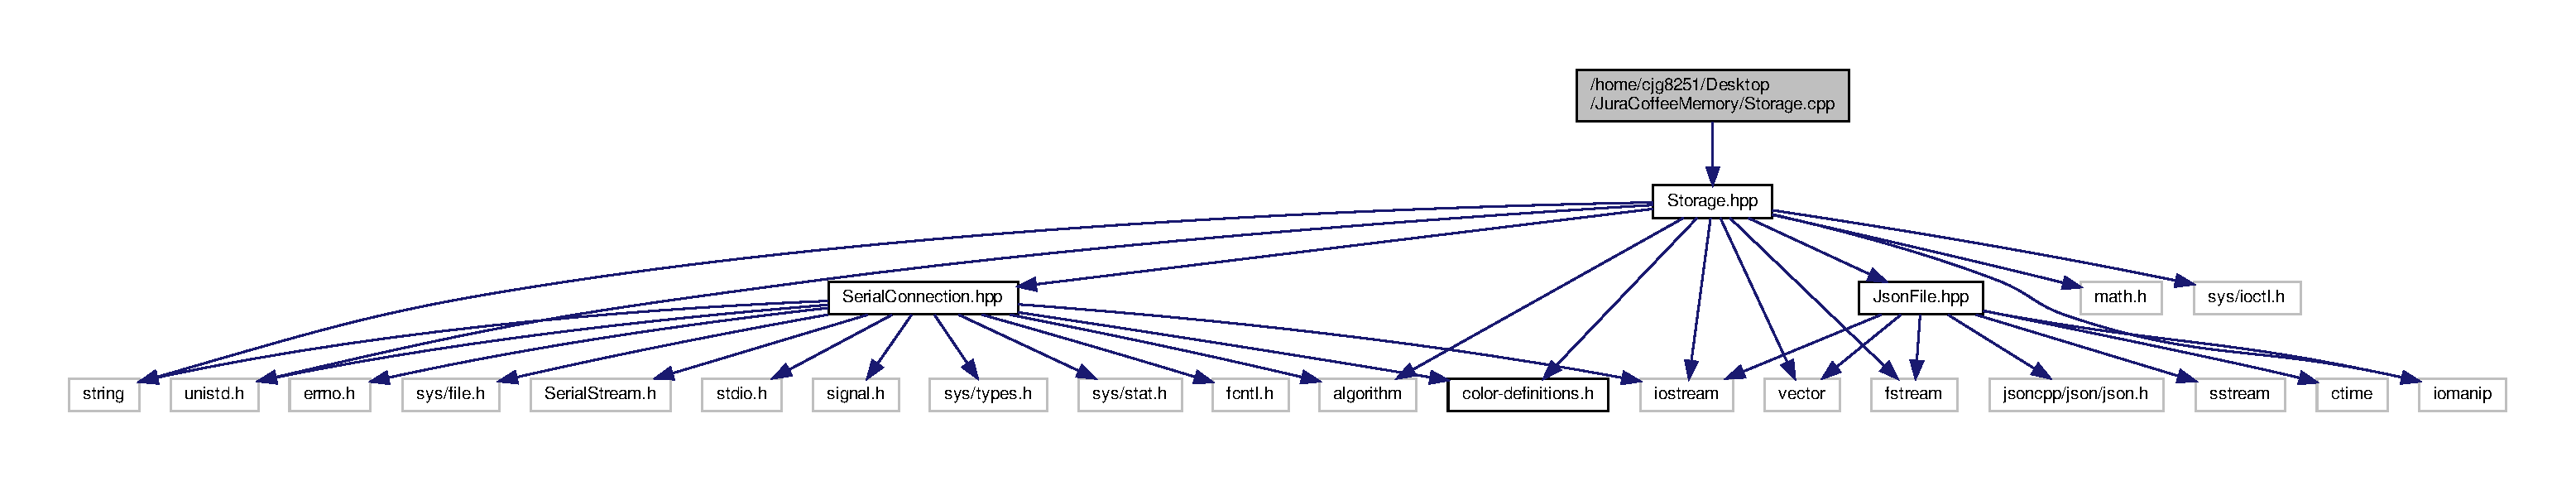
\includegraphics[width=350pt]{_storage_8cpp__incl}
\end{center}
\end{figure}

\section{/home/cjg8251/\+Desktop/\+Jura\+Coffee\+Memory/\+Storage.hpp-\/\+Dateireferenz}
\label{_storage_8hpp}\index{/home/cjg8251/\+Desktop/\+Jura\+Coffee\+Memory/\+Storage.\+hpp@{/home/cjg8251/\+Desktop/\+Jura\+Coffee\+Memory/\+Storage.\+hpp}}
{\ttfamily \#include $<$vector$>$}\newline
{\ttfamily \#include $<$iostream$>$}\newline
{\ttfamily \#include $<$fstream$>$}\newline
{\ttfamily \#include $<$string$>$}\newline
{\ttfamily \#include $<$unistd.\+h$>$}\newline
{\ttfamily \#include $<$iomanip$>$}\newline
{\ttfamily \#include $<$math.\+h$>$}\newline
{\ttfamily \#include $<$algorithm$>$}\newline
{\ttfamily \#include $<$sys/ioctl.\+h$>$}\newline
{\ttfamily \#include \char`\"{}Serial\+Connection.\+hpp\char`\"{}}\newline
{\ttfamily \#include \char`\"{}Json\+File.\+hpp\char`\"{}}\newline
{\ttfamily \#include \char`\"{}color-\/definitions.\+h\char`\"{}}\newline
Include-\/\+Abhängigkeitsdiagramm für Storage.\+hpp\+:
\nopagebreak
\begin{figure}[H]
\begin{center}
\leavevmode
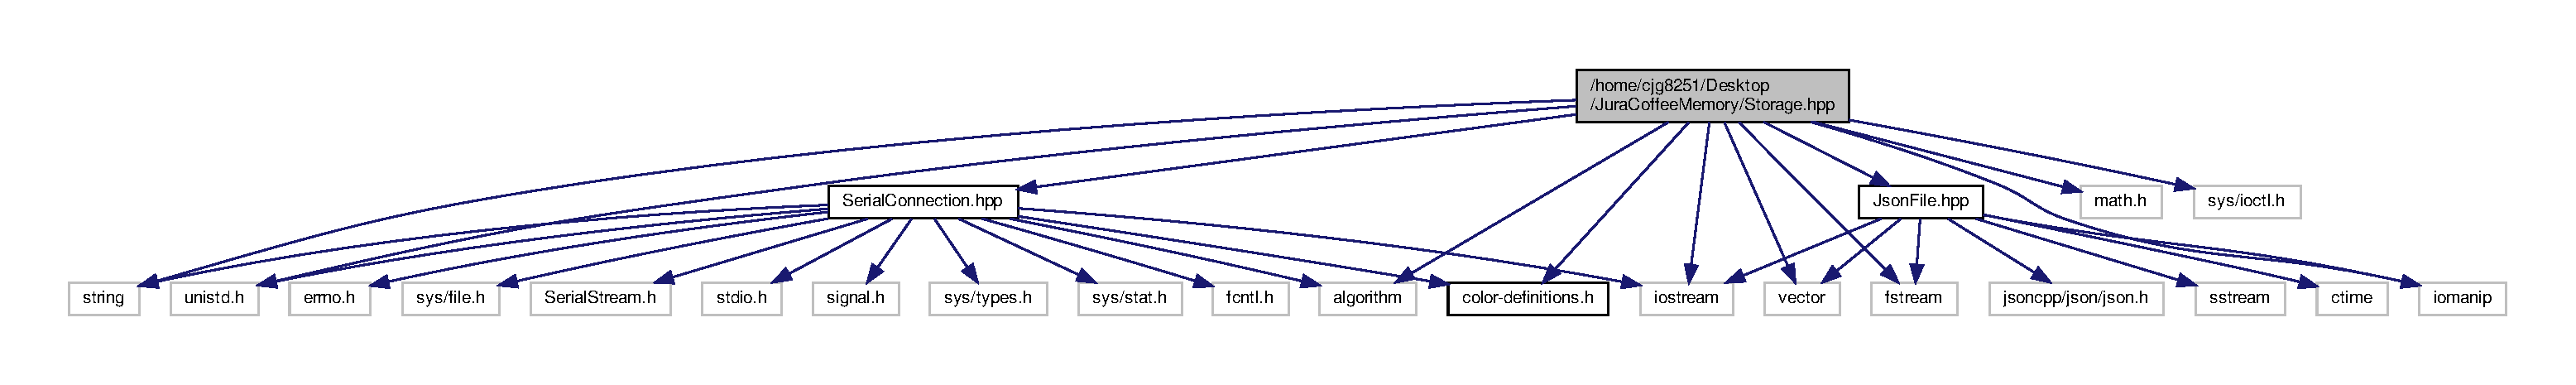
\includegraphics[width=350pt]{_storage_8hpp__incl}
\end{center}
\end{figure}
Dieser Graph zeigt, welche Datei direkt oder indirekt diese Datei enthält\+:
\nopagebreak
\begin{figure}[H]
\begin{center}
\leavevmode
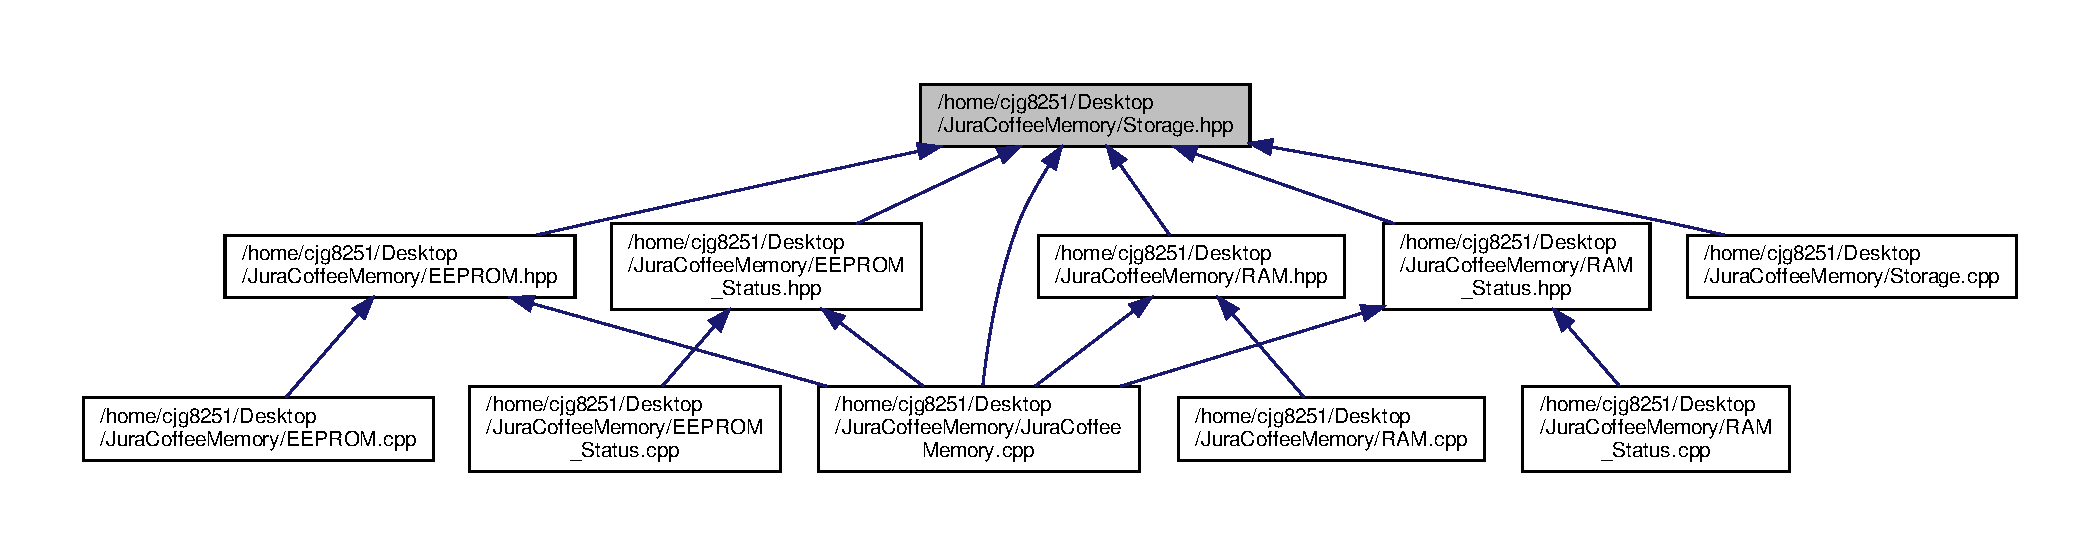
\includegraphics[width=350pt]{_storage_8hpp__dep__incl}
\end{center}
\end{figure}
\subsection*{Klassen}
\begin{DoxyCompactItemize}
\item 
class \textbf{ Storage}
\end{DoxyCompactItemize}

%--- End generated contents ---

% Index
\backmatter
\newpage
\phantomsection
\clearemptydoublepage
\addcontentsline{toc}{chapter}{Index}
\printindex

\end{document}
